%%%%%%%%%%%%%%%%%%%%%%%%%%%%%%%%%%%%%%%%%%%%%%%%%%%%%%%%%
%%   $RCSfile: hpsg04.tex,v $
%%  $Revision: 1.1 $
%%      $Date: 2004/08/11 09:53:01 $
%%     Author: Stefan Mueller (CL Uni Bremen)
%%    Purpose: 
%%   Language: LaTeX
%%%%%%%%%%%%%%%%%%%%%%%%%%%%%%%%%%%%%%%%%%%%%%%%%%%%%%%%%
%%
%% $Log: hpsg04.tex,v $
%% Revision 1.1  2004/08/11 09:53:01  stefan
%% *** empty log message ***
%%
%% Revision 1.1  2003/10/12 13:42:57  stefan
%% Initial revision
%%
%%%%%%%%%%%%%%%%%%%%%%%%%%%%%%%%%%%%%%%%%%%%%%%%%%%%%%%%%

\documentclass[11pt,a4paper,fleqn]{article}
\usepackage{times}
\thispagestyle{empty}



\usepackage[T1]{fontenc}   % Silbentrennung

\usepackage{8bit}

\usepackage[bookmarks=true,bookmarksopen=true,%
breaklinks=true,%
draft=false,colorlinks=false,plainpages=false,hyperfootnotes=false,%
linkcolor=black,%
pagecolor=black,%
pdfauthor={Stefan M�ller (Editor)},%
pdftitle={Proceedings of the HPSG05 Conference},%
pdfkeywords={HPSG}%,
pdftex=true%
%ps2pdf=true  %ohne diesen Treiber geht der Zeilenumbruch in URLs
]{hyperref}% for pdf files

\usepackage{pdfpages}


\hypersetup{colorlinks=false, pdfborder={0 0 0}}

\begin{document}

\begin{center}
{\Large
                Proceedings of the HPSG05 Conference\\[\baselineskip]

                Department of Informatics, University of Lisbon\\[\baselineskip]

                        Stefan M{\"u}ller (Editor)\\[\baselineskip]

                                2005\\[\baselineskip]

                          CSLI Publications\\[\baselineskip]

              http://csli-publications.stanford.edu/
}
\end{center}
\newpage
\tableofcontents

\newpage

\section{Editor's Note}

The 12th International Conference on Head-Driven Phrase Structure Grammar (2005) was held at
the Department of Informatics, University of Lisbon in Portugal.

The conference featured 2 invited talks, 18 papers, 2 alternate papers, and 6 posters
selected by the program committee 
(Raul Aranovich,
Doug Arnold,
Emily Bender,
Olivier Bonami,
Ant�nio Branco,
Berthold Crysmann,
Anke Holler,
Valia Kordoni,
Palmira Marrafa,
Tsuneko Nakazawa,
Gerald Penn,
Alexander Rosen,
Manfred Sailer (chair),
Gautam Sengupta,
Jesse Tseng,
Stephen Wechsler, and
Shuly Winter). 
A workshop on \emph{Binding Theory and Invariants in Anaphoric Relations} was attached to the conference. It featured one invited talk
and 12 papers, selected by the workshop program committee (Pilar Barbosa,
Ant�nio Branco,chair,
Rejean Canac-Marquis,
Mary Dalrymple,
Martin Evearert,
Volker Gast,
Lars Hellan,
Ehrard Hinrichs,
Yan Huang,
Tibor Kiss,
Frank Keller,
Valia Kordoni,
Maria Pinango,
Carl Pollard,
Janina Rad�o,
Eric Reuland,
Jeffrey Runner,
Ivan Sag,
Roland Stuckardt,
Ping Xue).

In total there were 39 submissions to the main conference and 13 sbmissions to the
workshop. 
We want to thank the respective program committees for putting this nice program together.

Thanks go to Ant�nio Branco, who was in charge of local arrangements.

As in the past years the contributions to the conference proceedings are based on the five page abstract
that was reviewed by the respective program committees, but there is no additional reviewing of the
longer contribution to the proceedings.
To ensure easy access and fast publication we have chosen an electronic format.

The proceedings include all the papers except those by 
Frank Keller and Theodora Alexopoulou, Stefan M�ller and Eric Reuland. Nurit Melnik submitted
an extended abstract, the full paper will appear in a Research on Language and Computation.


\newpage
\part{Contributions to the Main Conference}

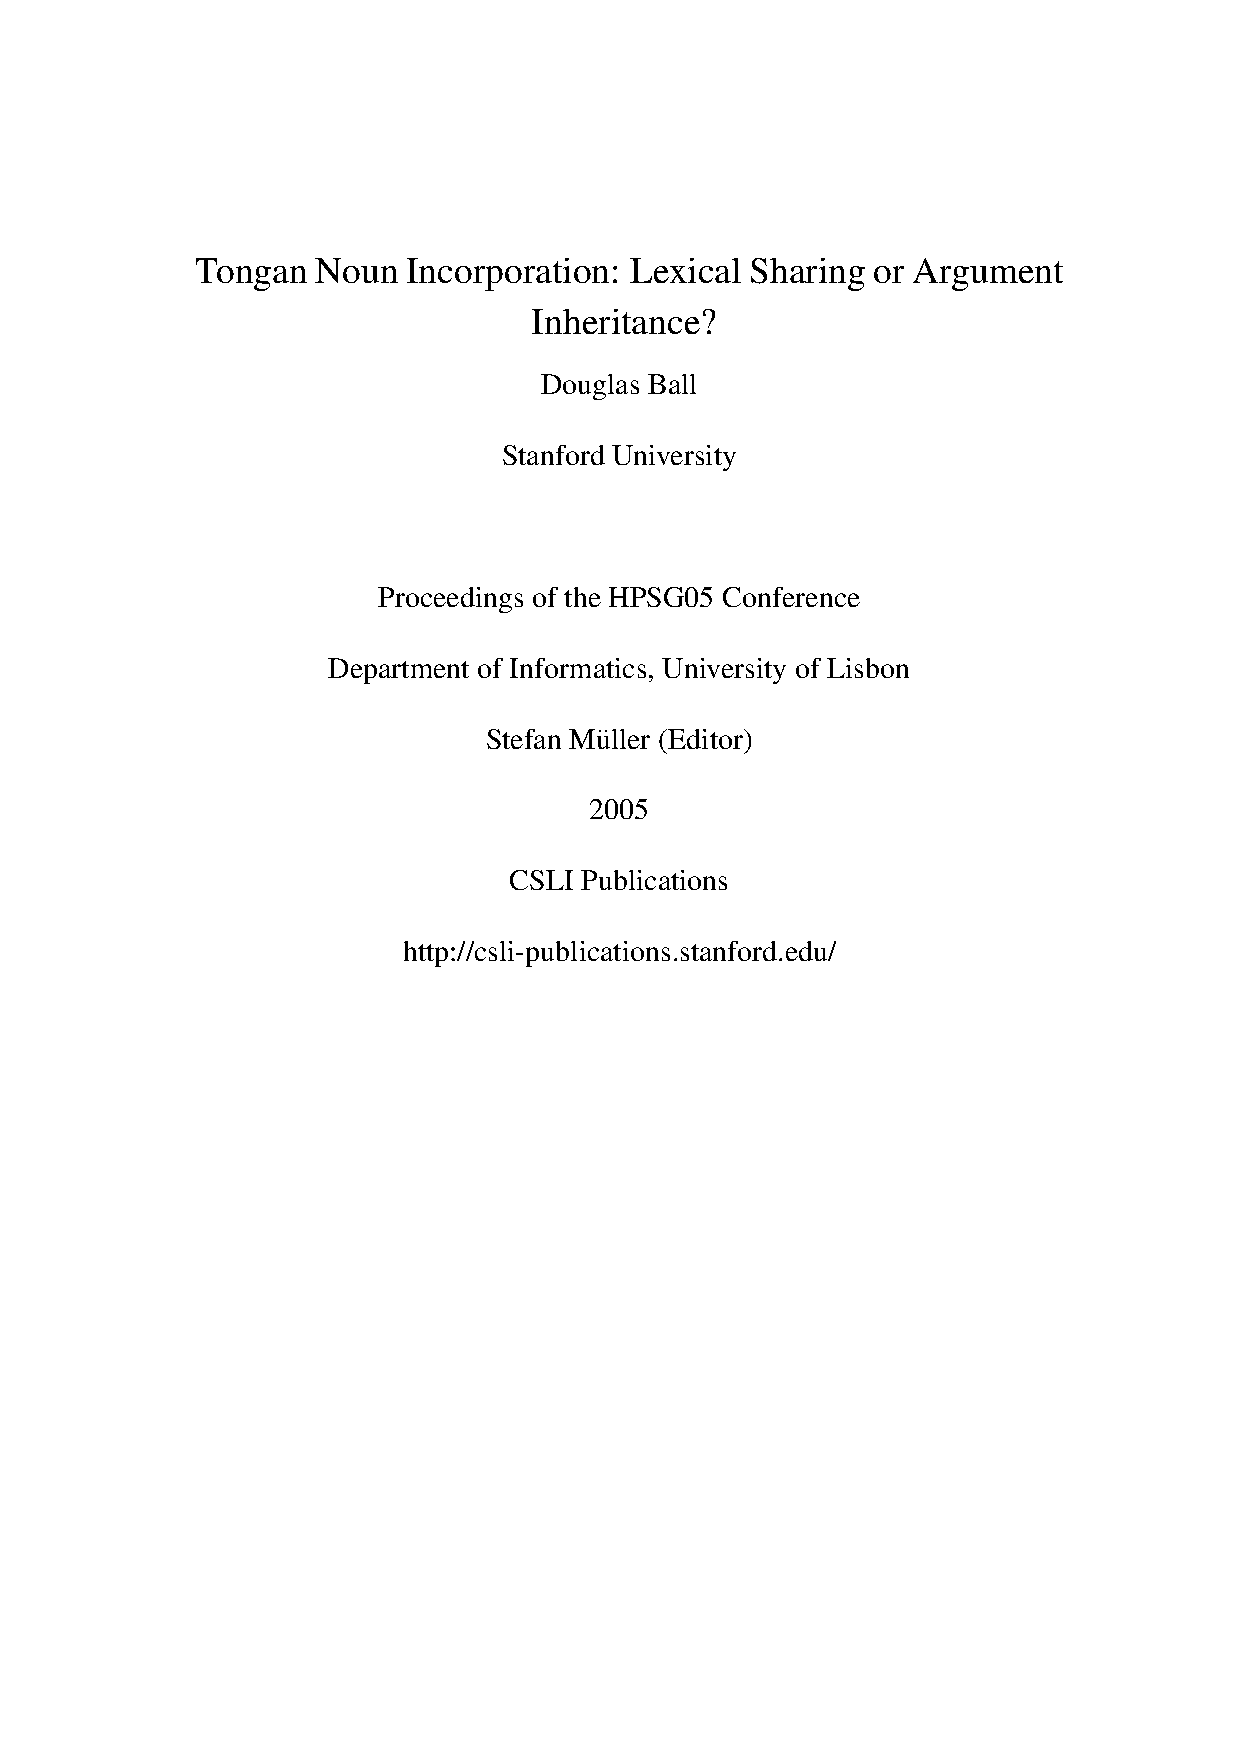
\includepdf[pages=-,pagecommand=\thispagestyle{plain},
            addtotoc={1,section,1,
            {Douglas Ball: Tongan Noun Incorporation: Lexical Sharing or Argument Inheritance?},
             ball}]{ball.pdf}

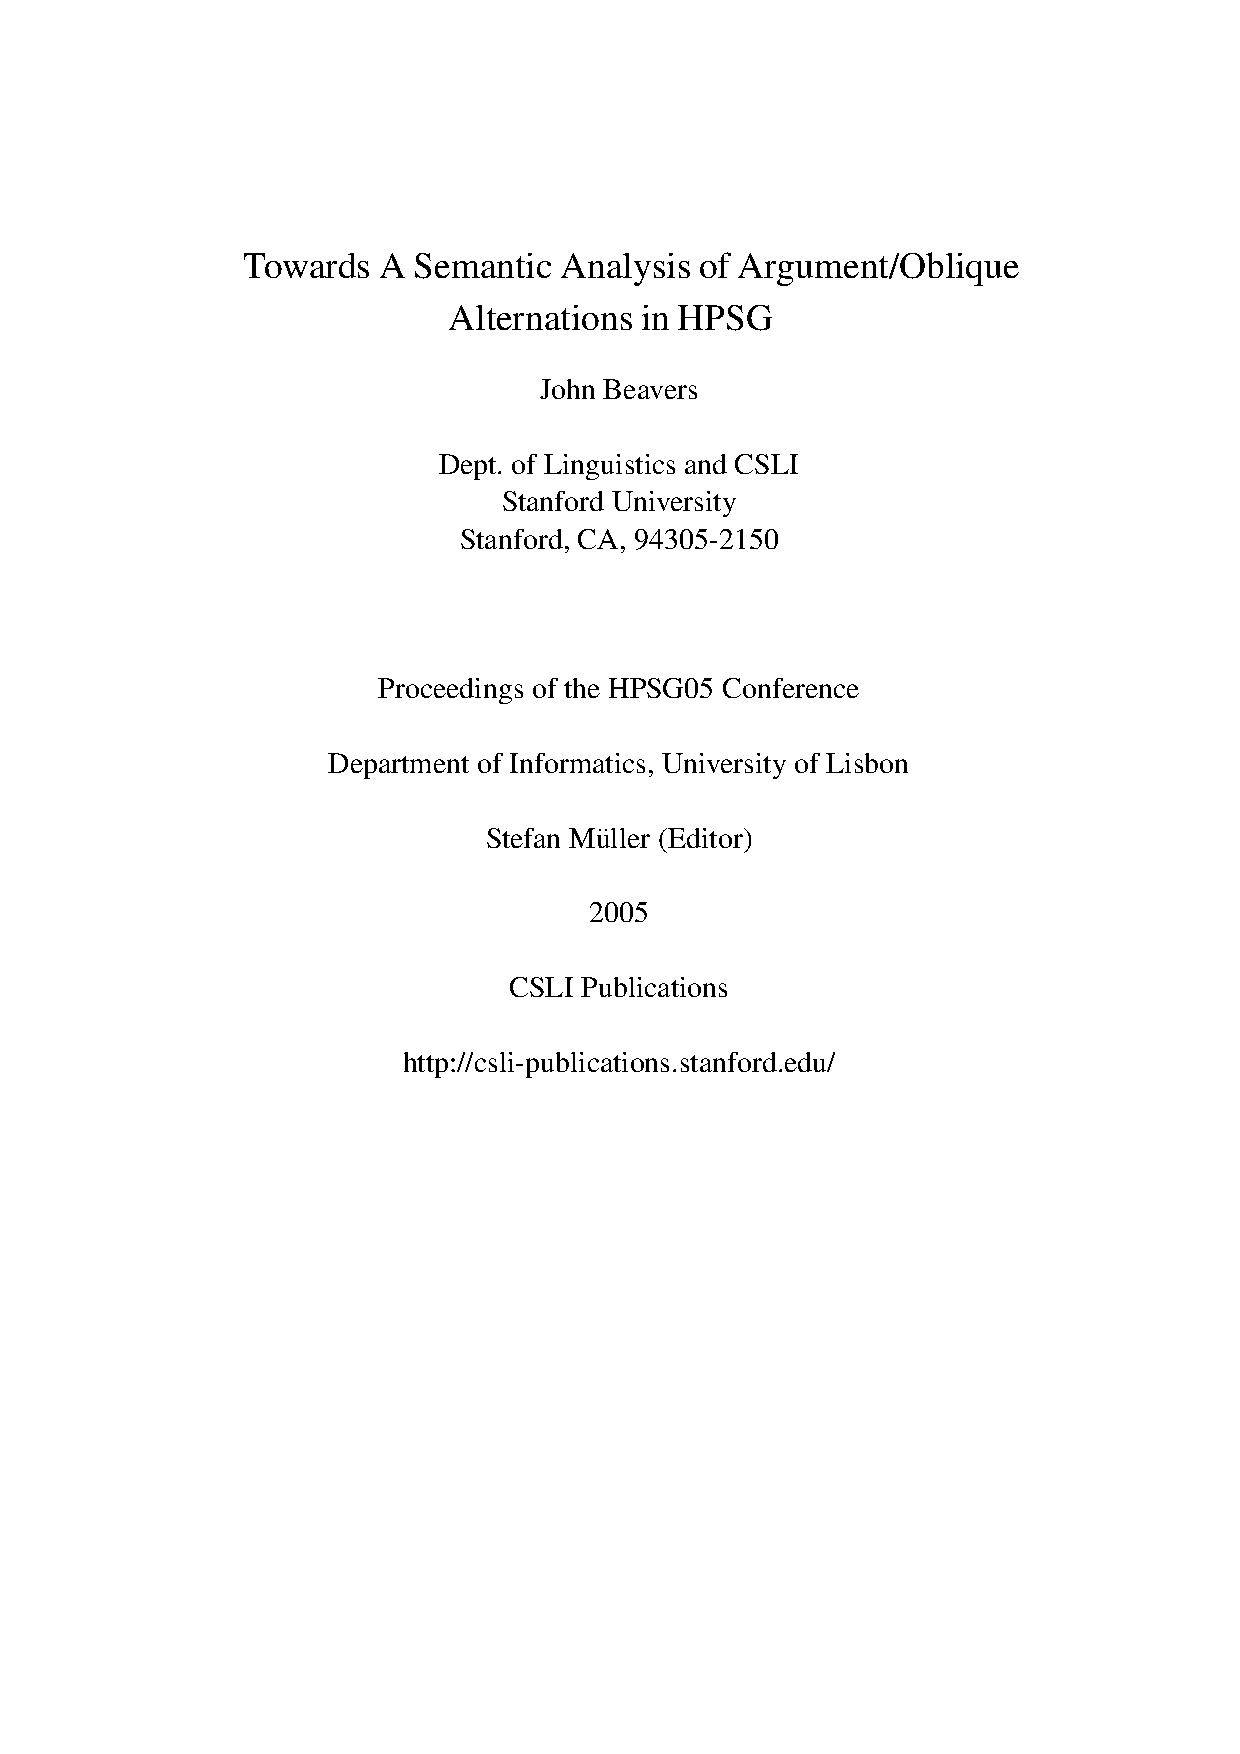
\includepdf[pages=-,pagecommand=\thispagestyle{plain},
            addtotoc={1,section,1,
            {John Beavers: Towards A Semantic Analysis of Argument/Oblique Alternations in HPSG},
             beavers}]{beavers.pdf}

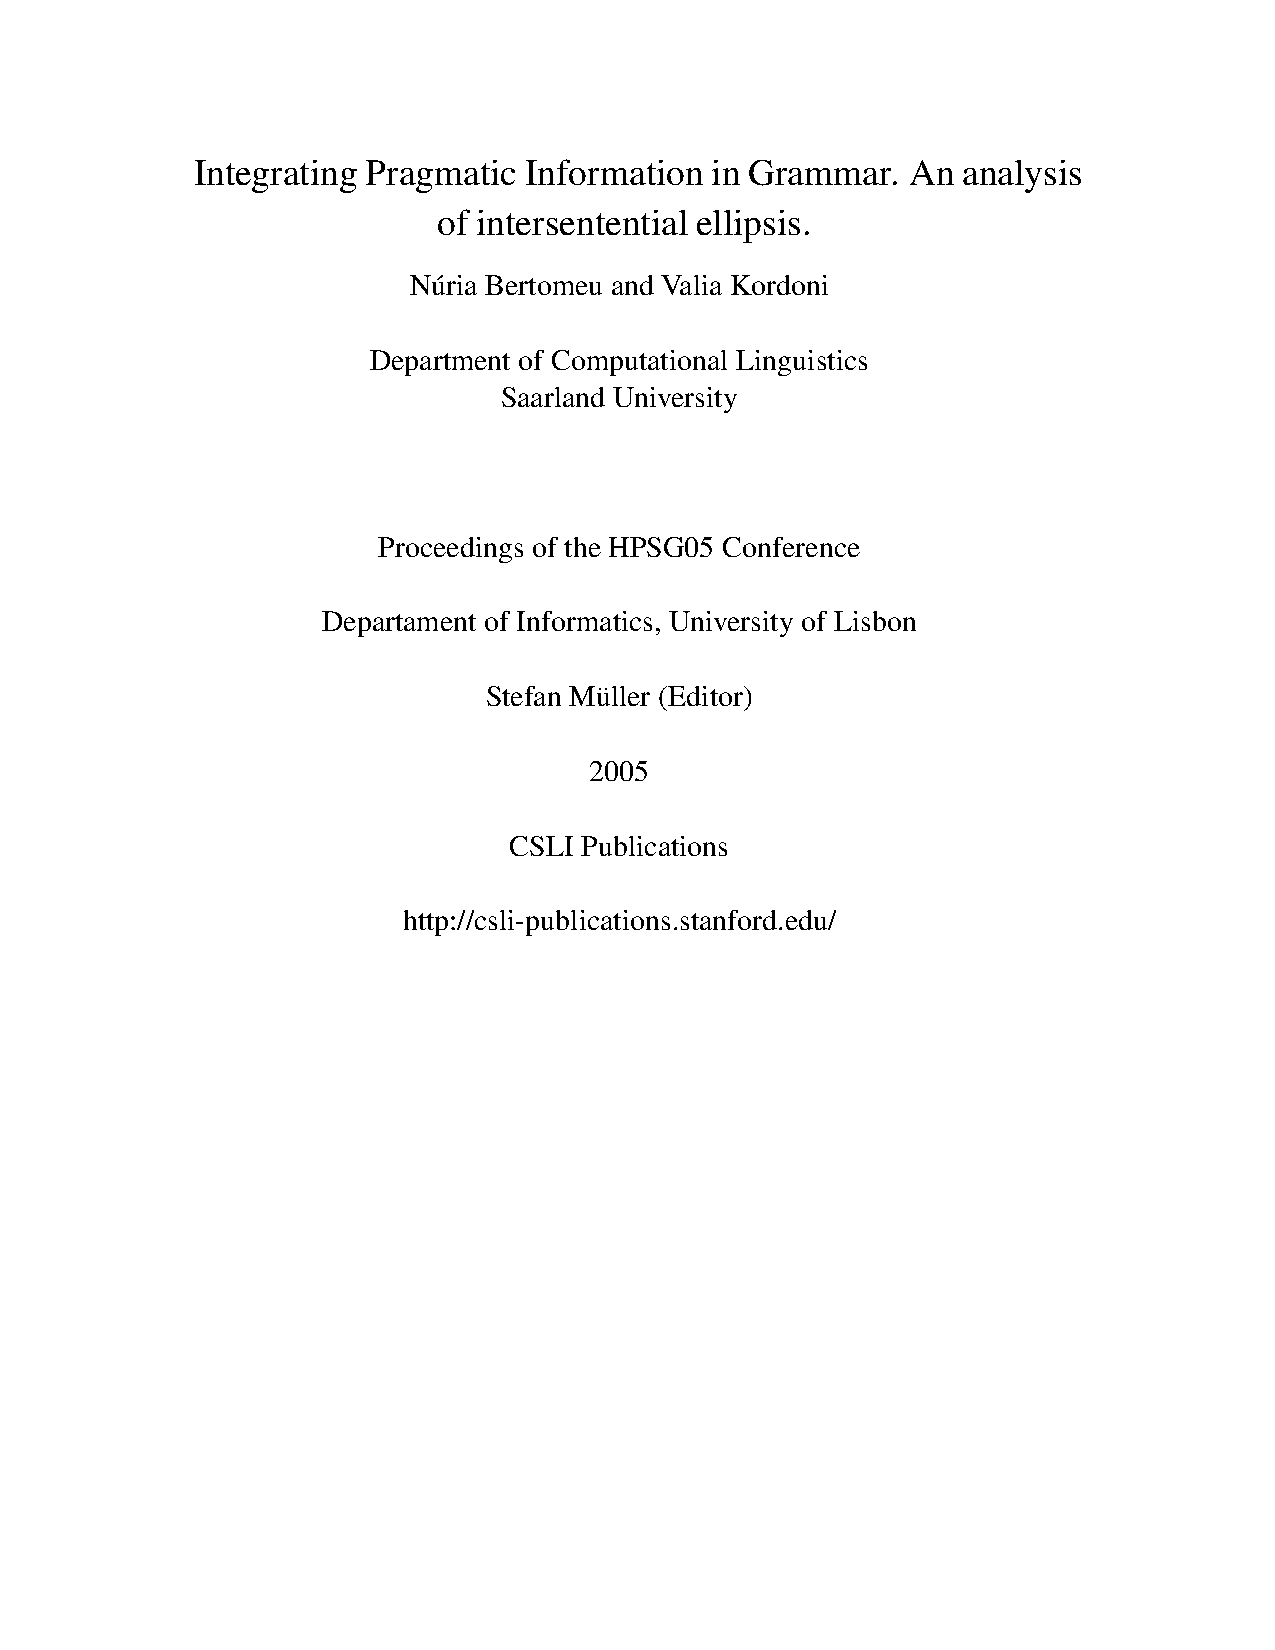
\includepdf[pages=-,pagecommand=\thispagestyle{plain},
            addtotoc={1,section,1,
            {N�ria Bertomeu and Valia Kordoni: Integrating Pragmatic Information in  Grammar. An Analysis of Intersentential Ellipsis},
             bk}]{bertomeu_kordoni.pdf}

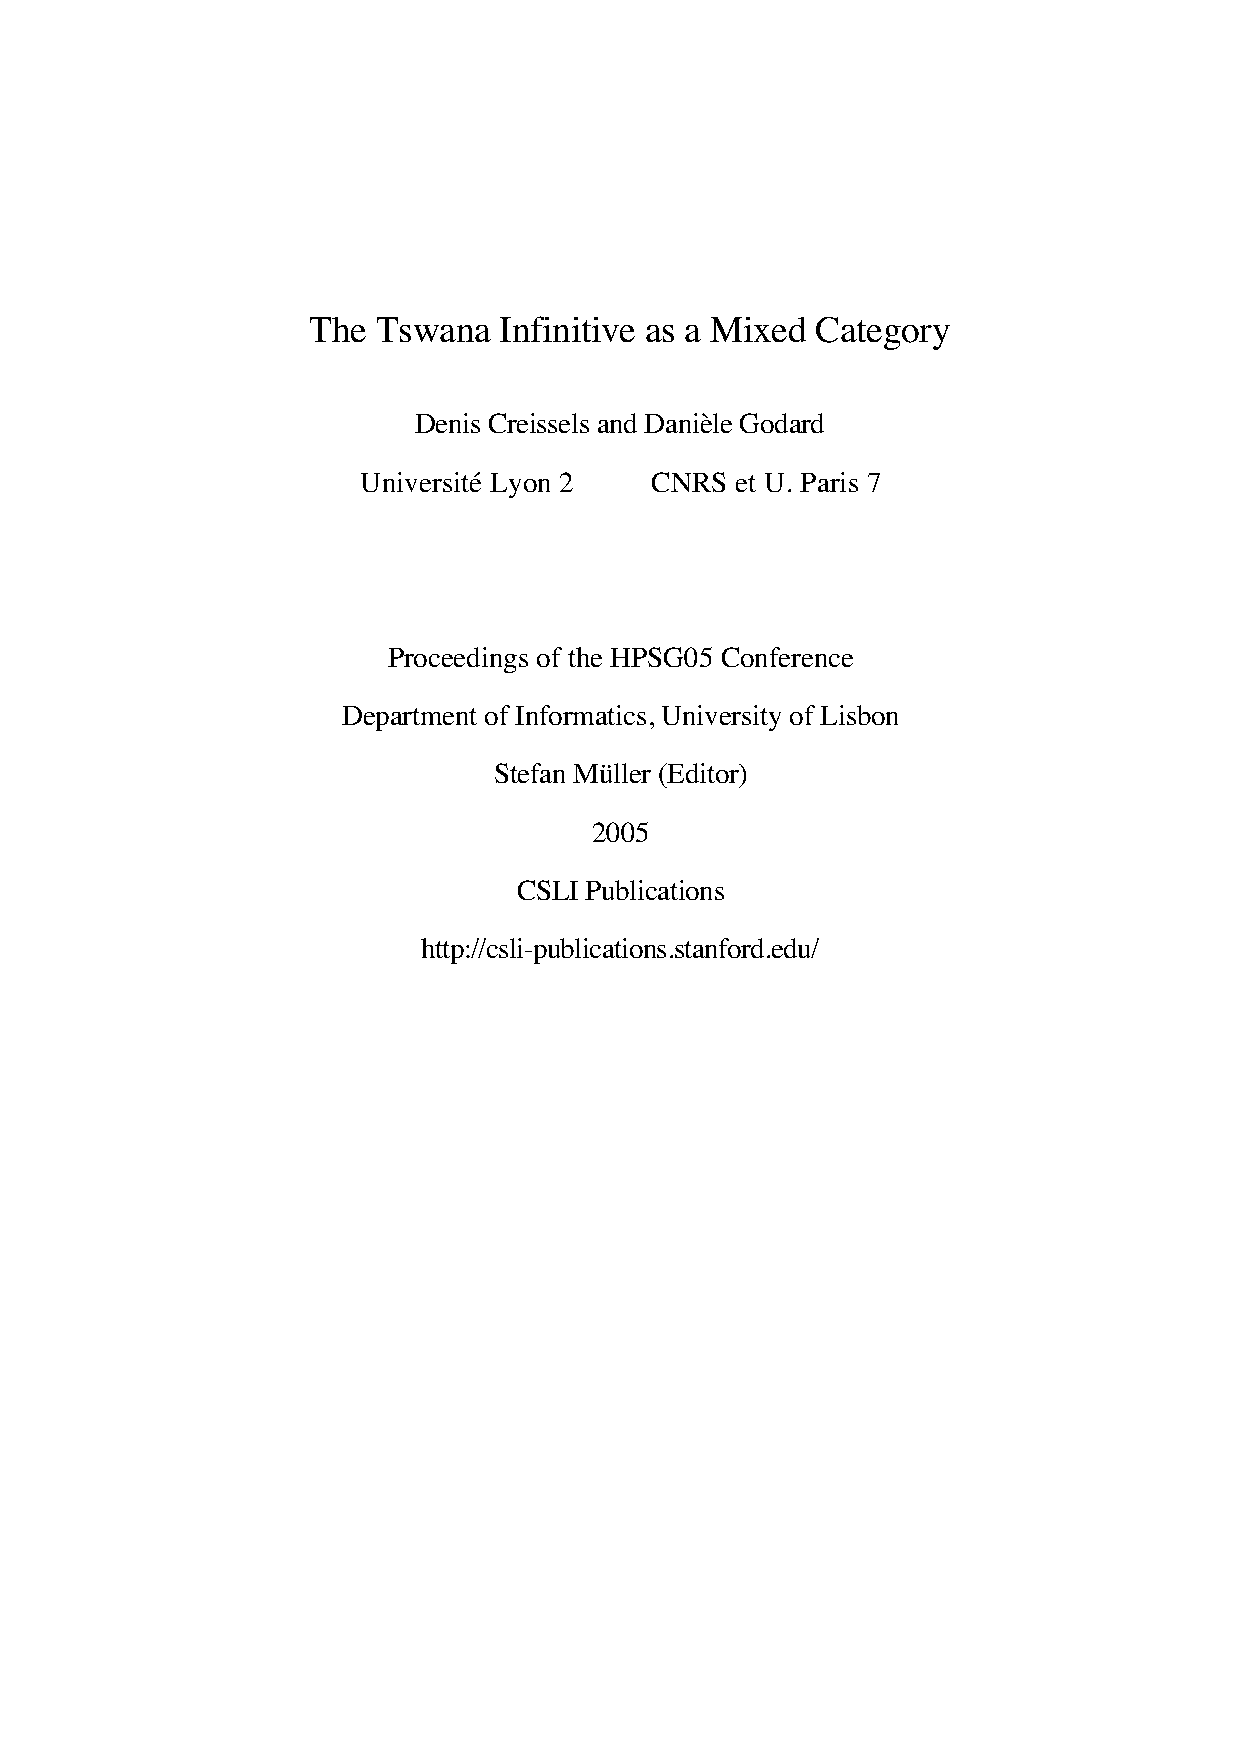
\includepdf[pages=-,pagecommand=\thispagestyle{plain},
            addtotoc={1,section,1,
            {Denis Creissels and Dani�le Godard: The Tswana Infinitive as a Mixed Category},
             cg}]{creissels-godard.pdf}


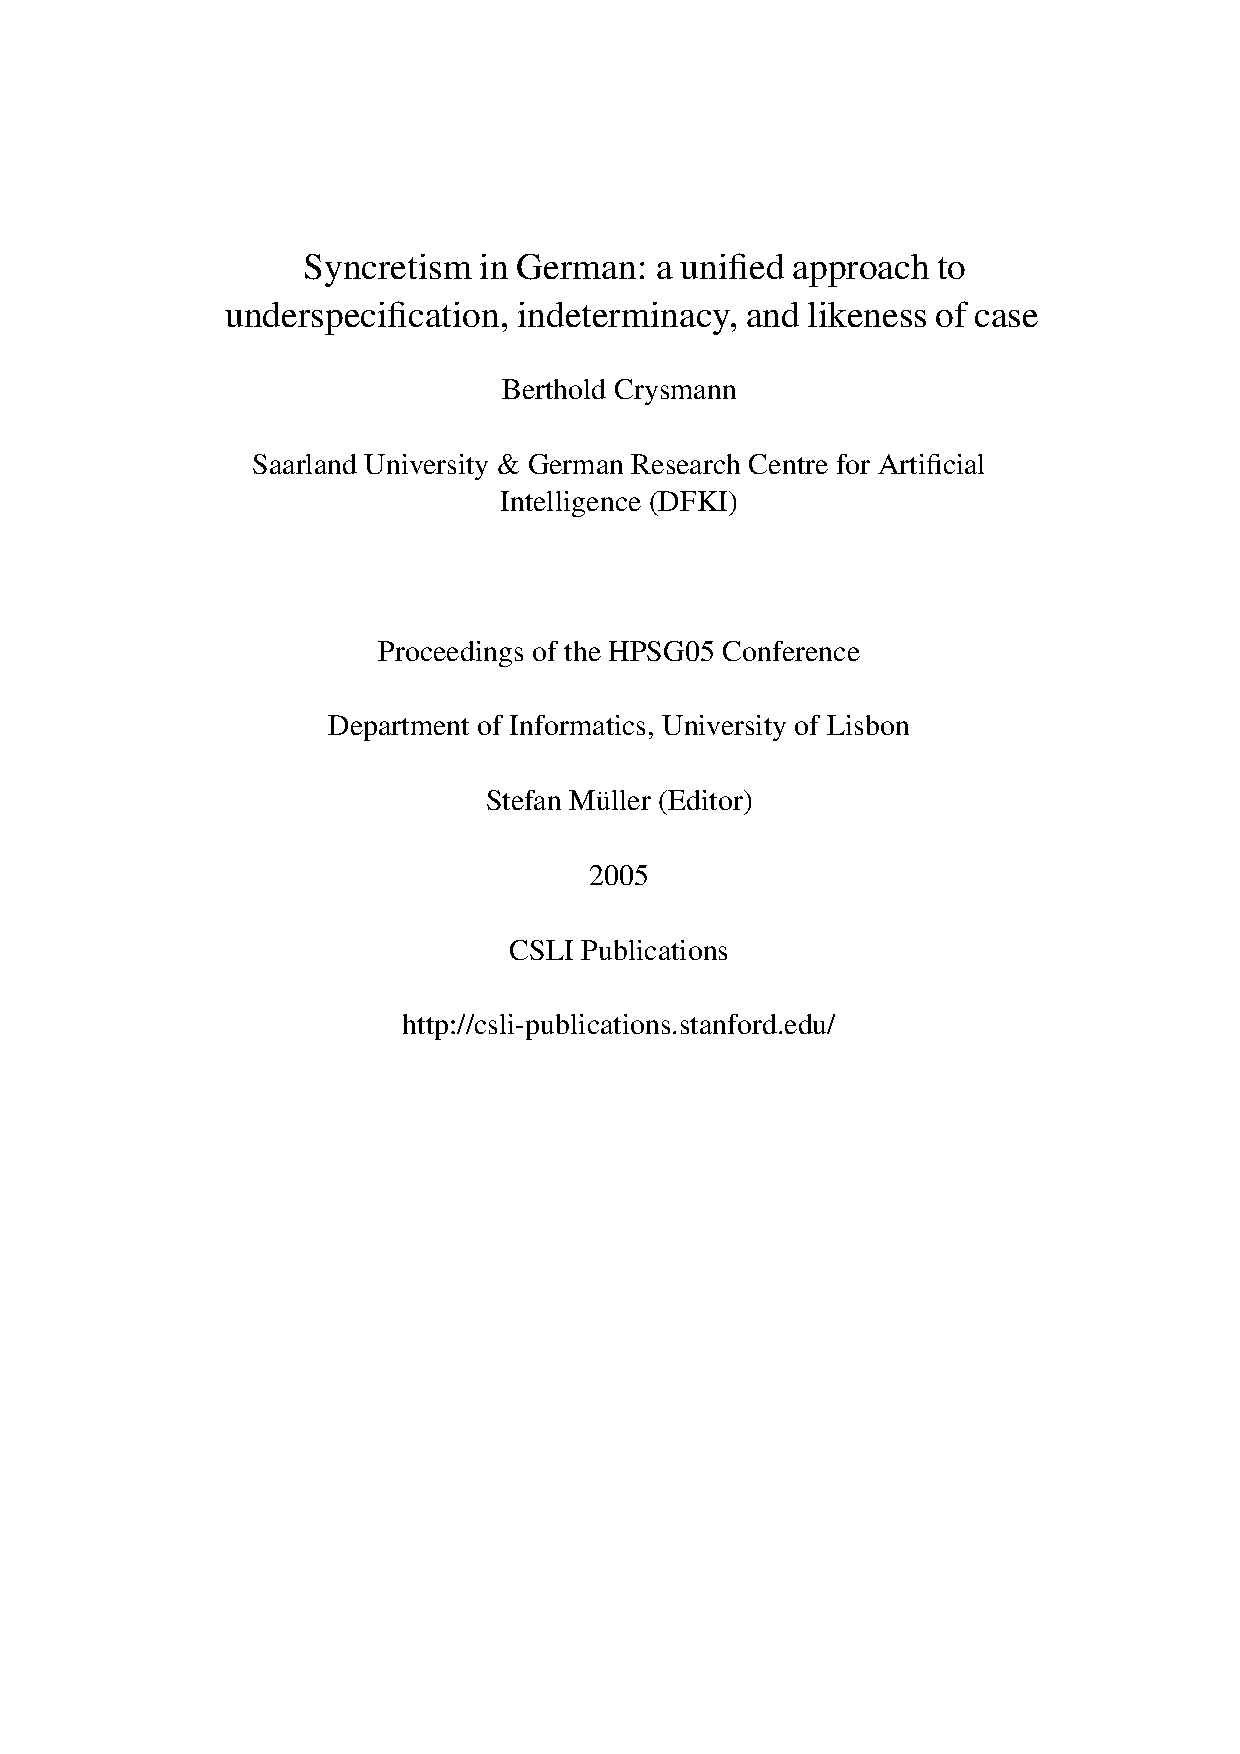
\includepdf[pages=-,pagecommand=\thispagestyle{plain},
            addtotoc={1,section,1,
            {Berthold Crysmann: Syncretism in German: A Unified Approach to Underspecification, Indeterminacy, and Likeness of Case},
             crysmann}]{crysmann.pdf}


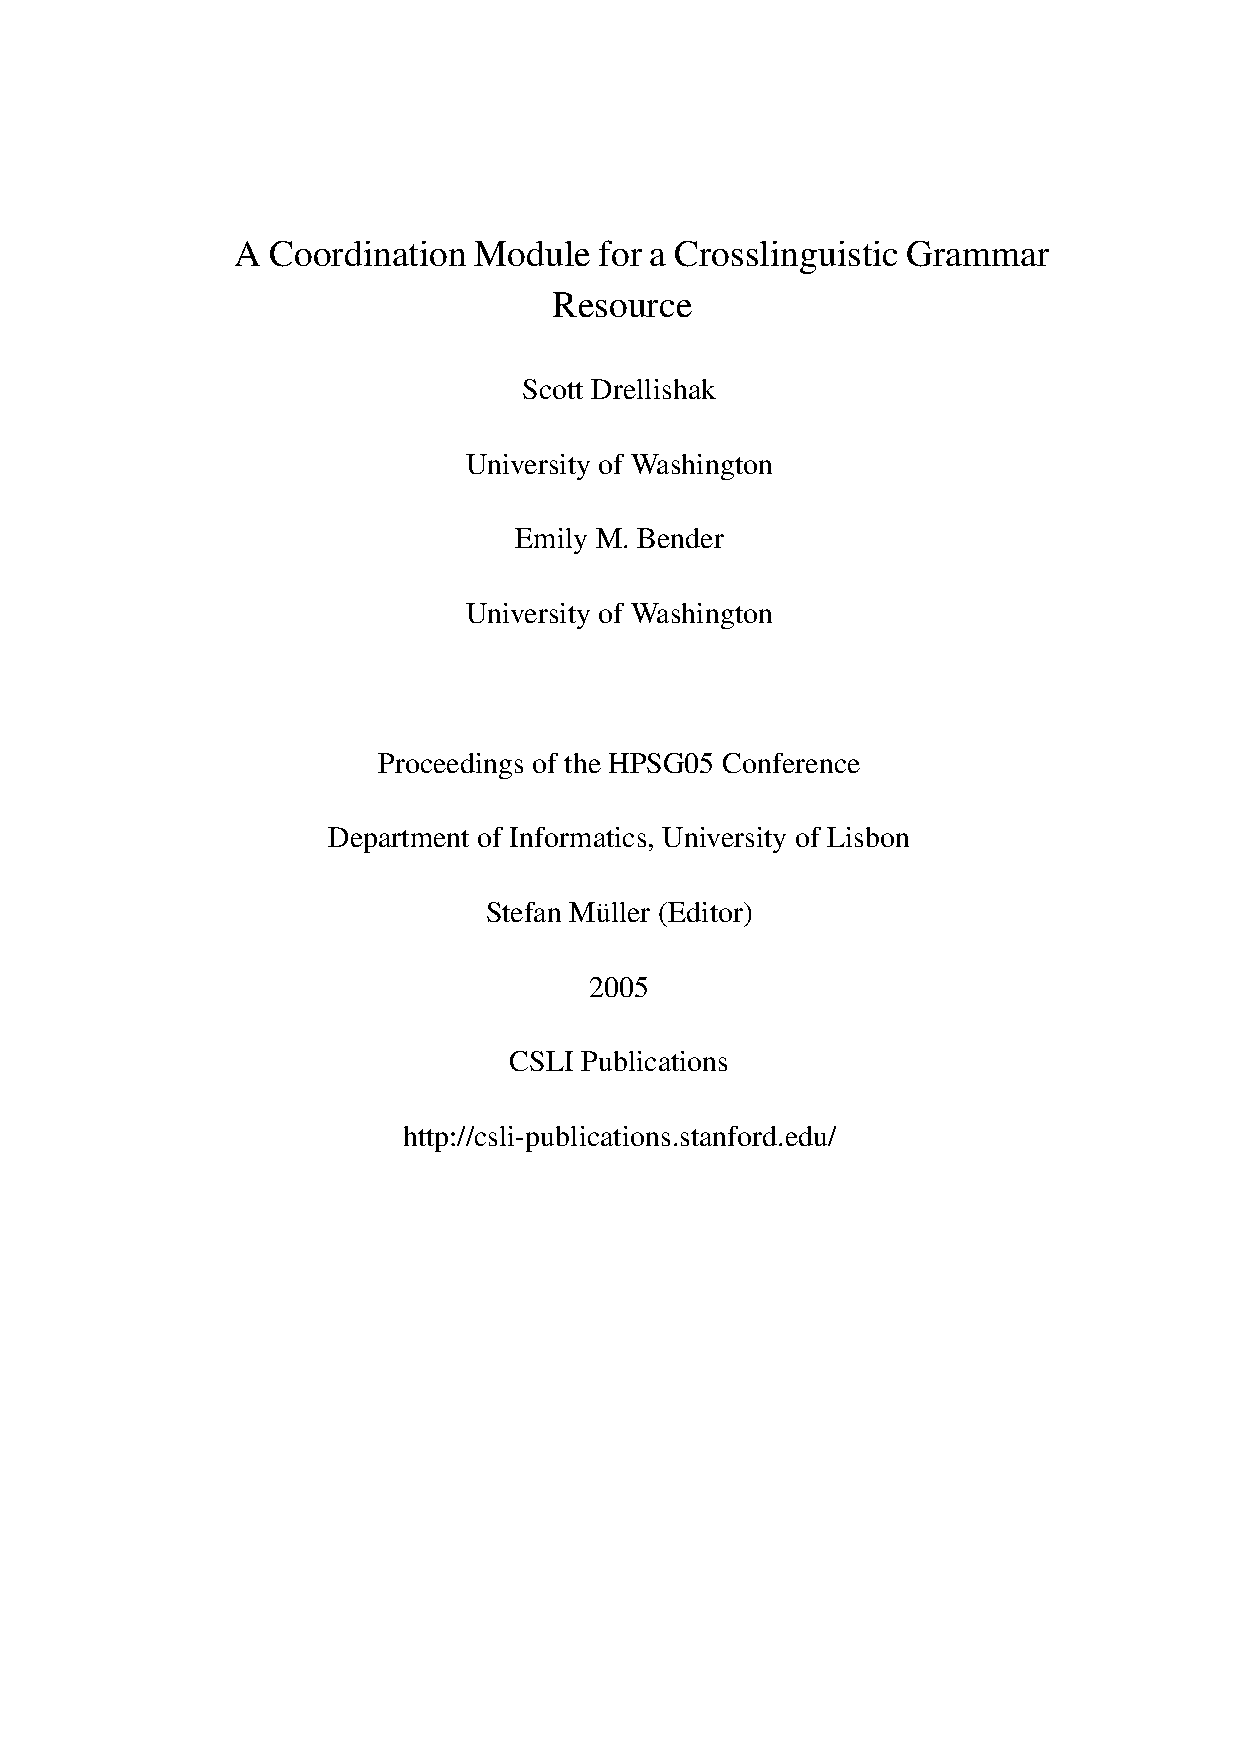
\includepdf[pages=-,pagecommand=\thispagestyle{plain},
            addtotoc={1,section,1,
            {Scott Drellishak and Emily M. Bender: A Coordination Module for a Crosslinguistic Grammar Resource},
             db}]{drellishak-bender.pdf}

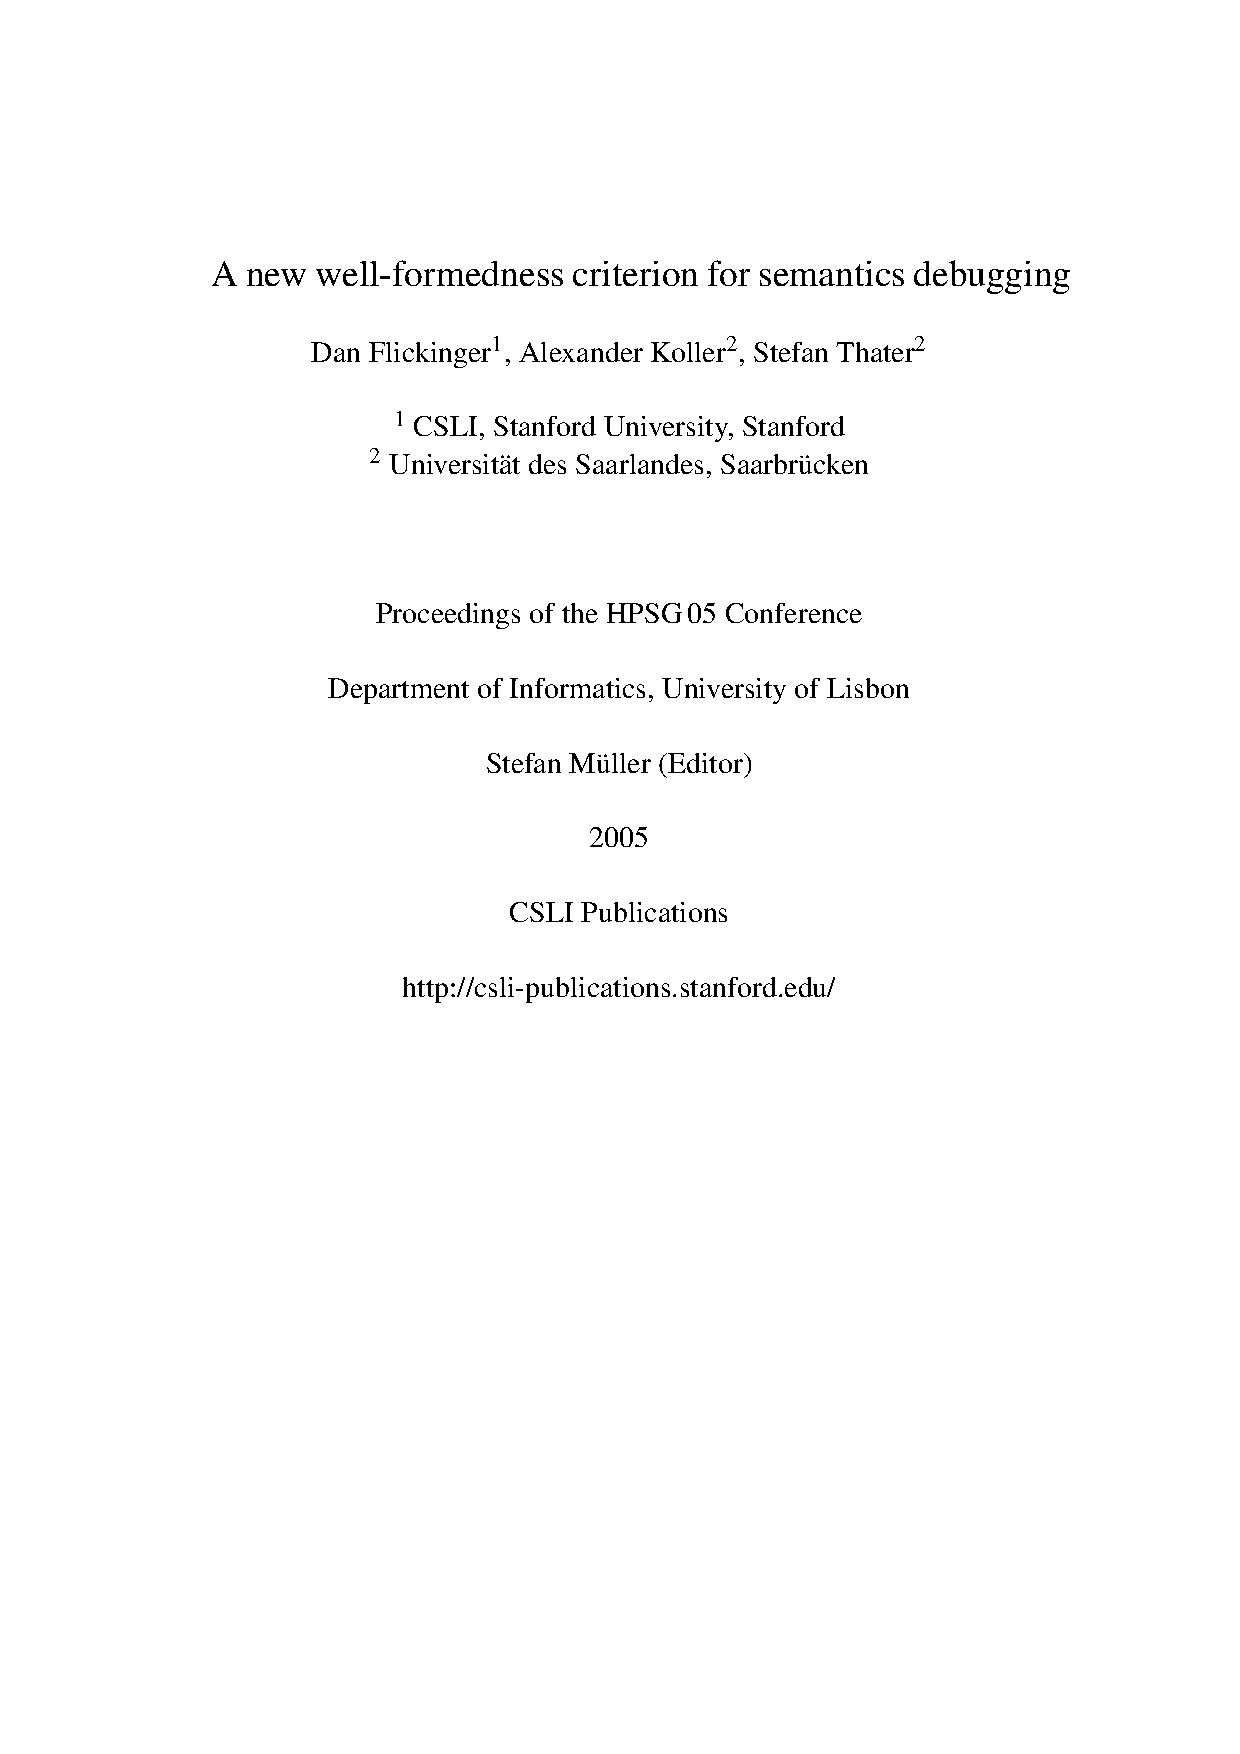
\includepdf[pages=-,pagecommand=\thispagestyle{plain},
            addtotoc={1,section,1,
            {Dan Flickinger, Alexander Koller, and Stafan Thater: A New Well-Formedness Criterion for Semantics Debugging},
             fkt}]{flickinger-koller-thater.pdf}


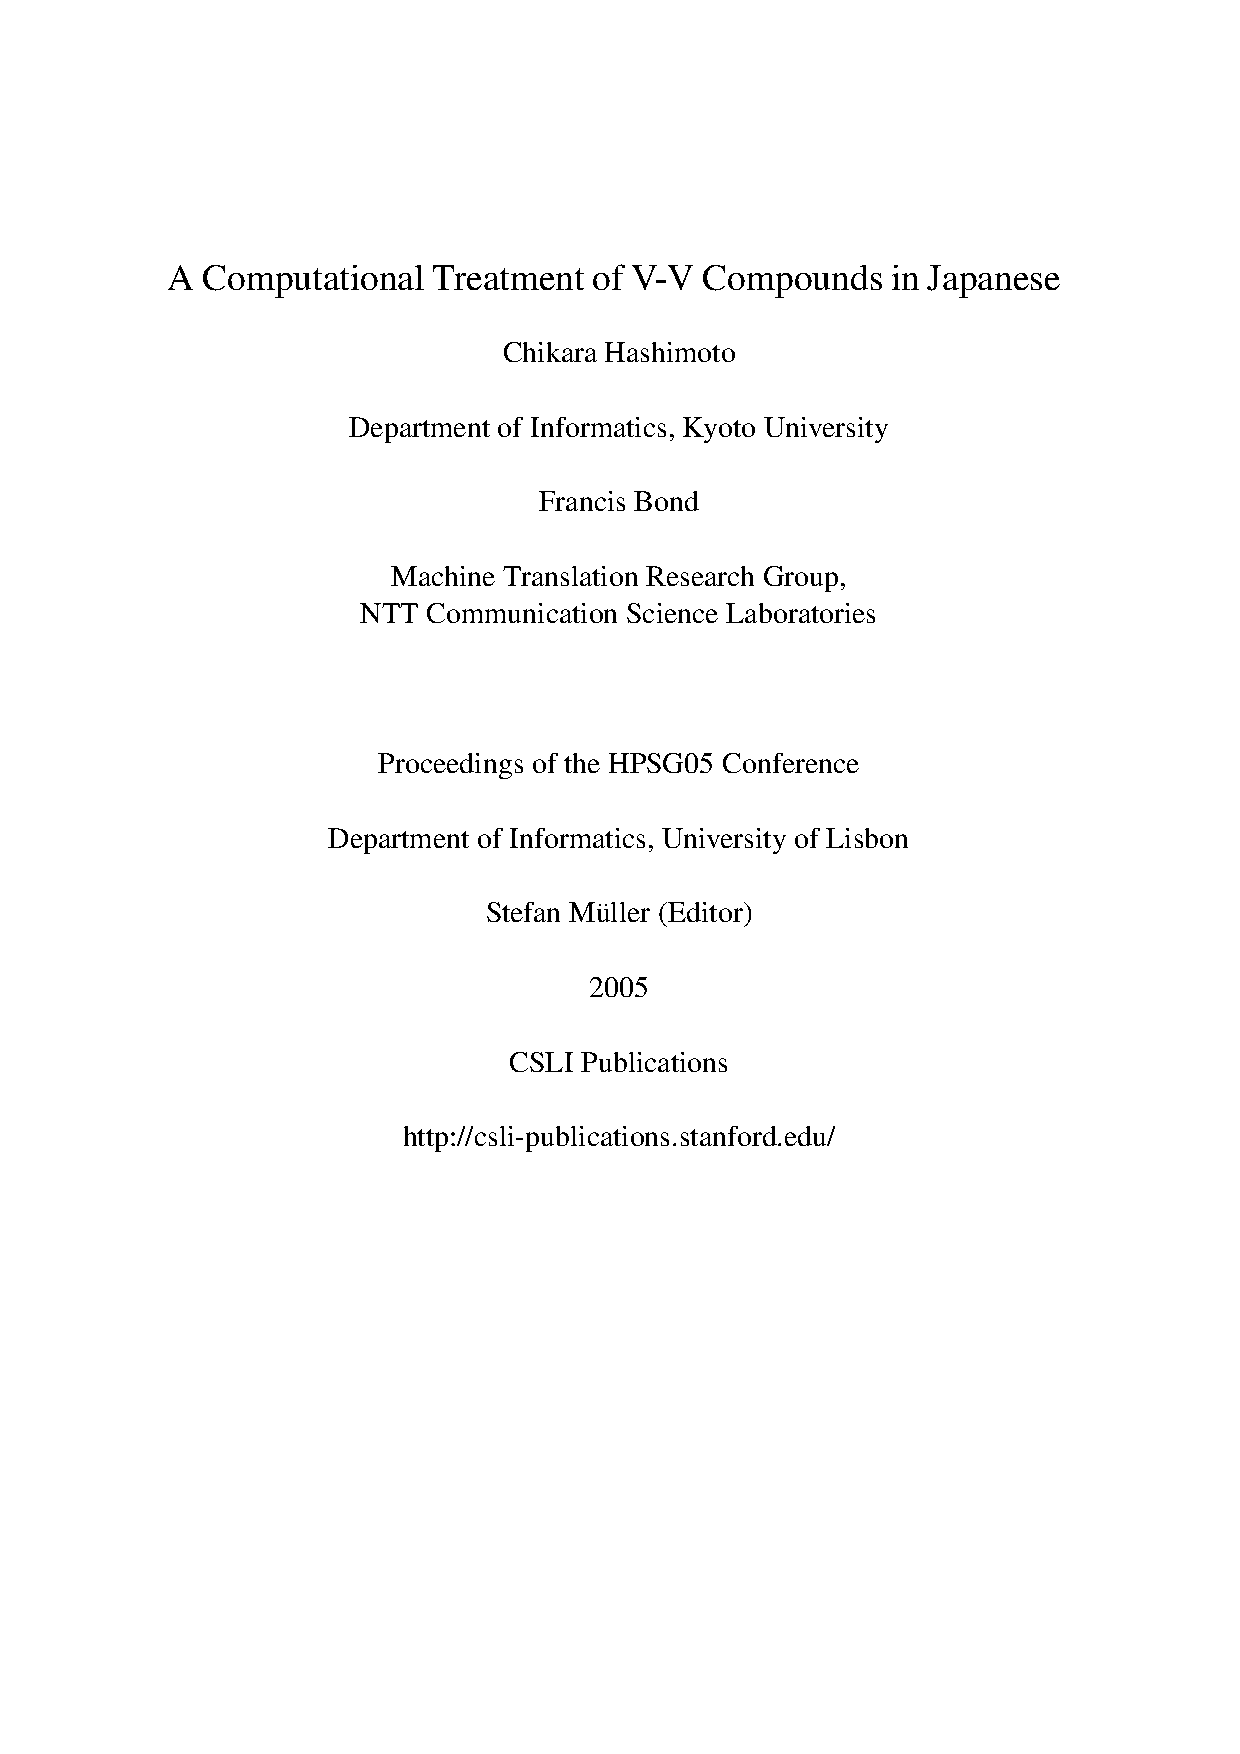
\includepdf[pages=-,pagecommand=\thispagestyle{plain},
            addtotoc={1,section,1,
            {Chikara Hashimoto and Francis Bond: A Computational Treatment of V-V Compounds in Japanese},
             hb}]{hashimoto-bond.pdf}


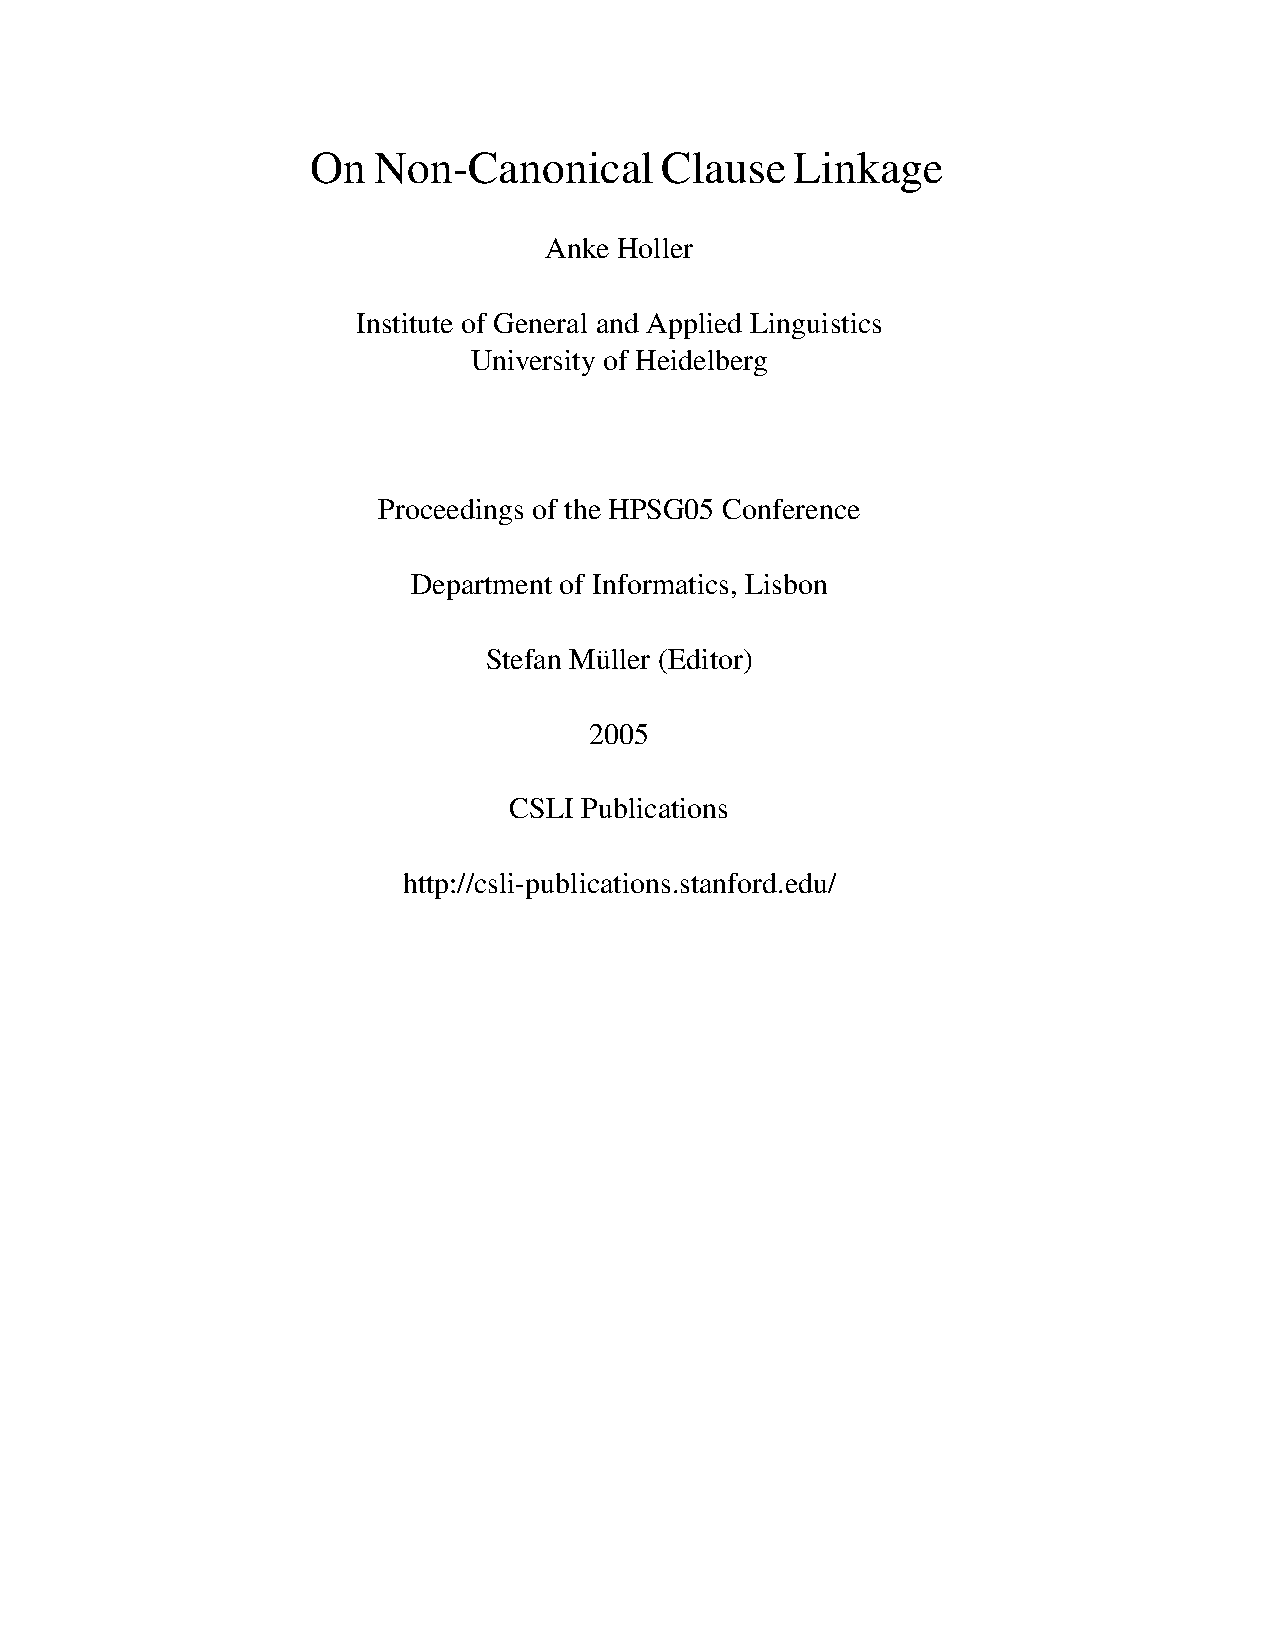
\includepdf[pages=-,pagecommand=\thispagestyle{plain},
            addtotoc={1,section,1,
            {Anke Holler: On Non-Canonical Clause Linkage},
             holler}]{holler.pdf}

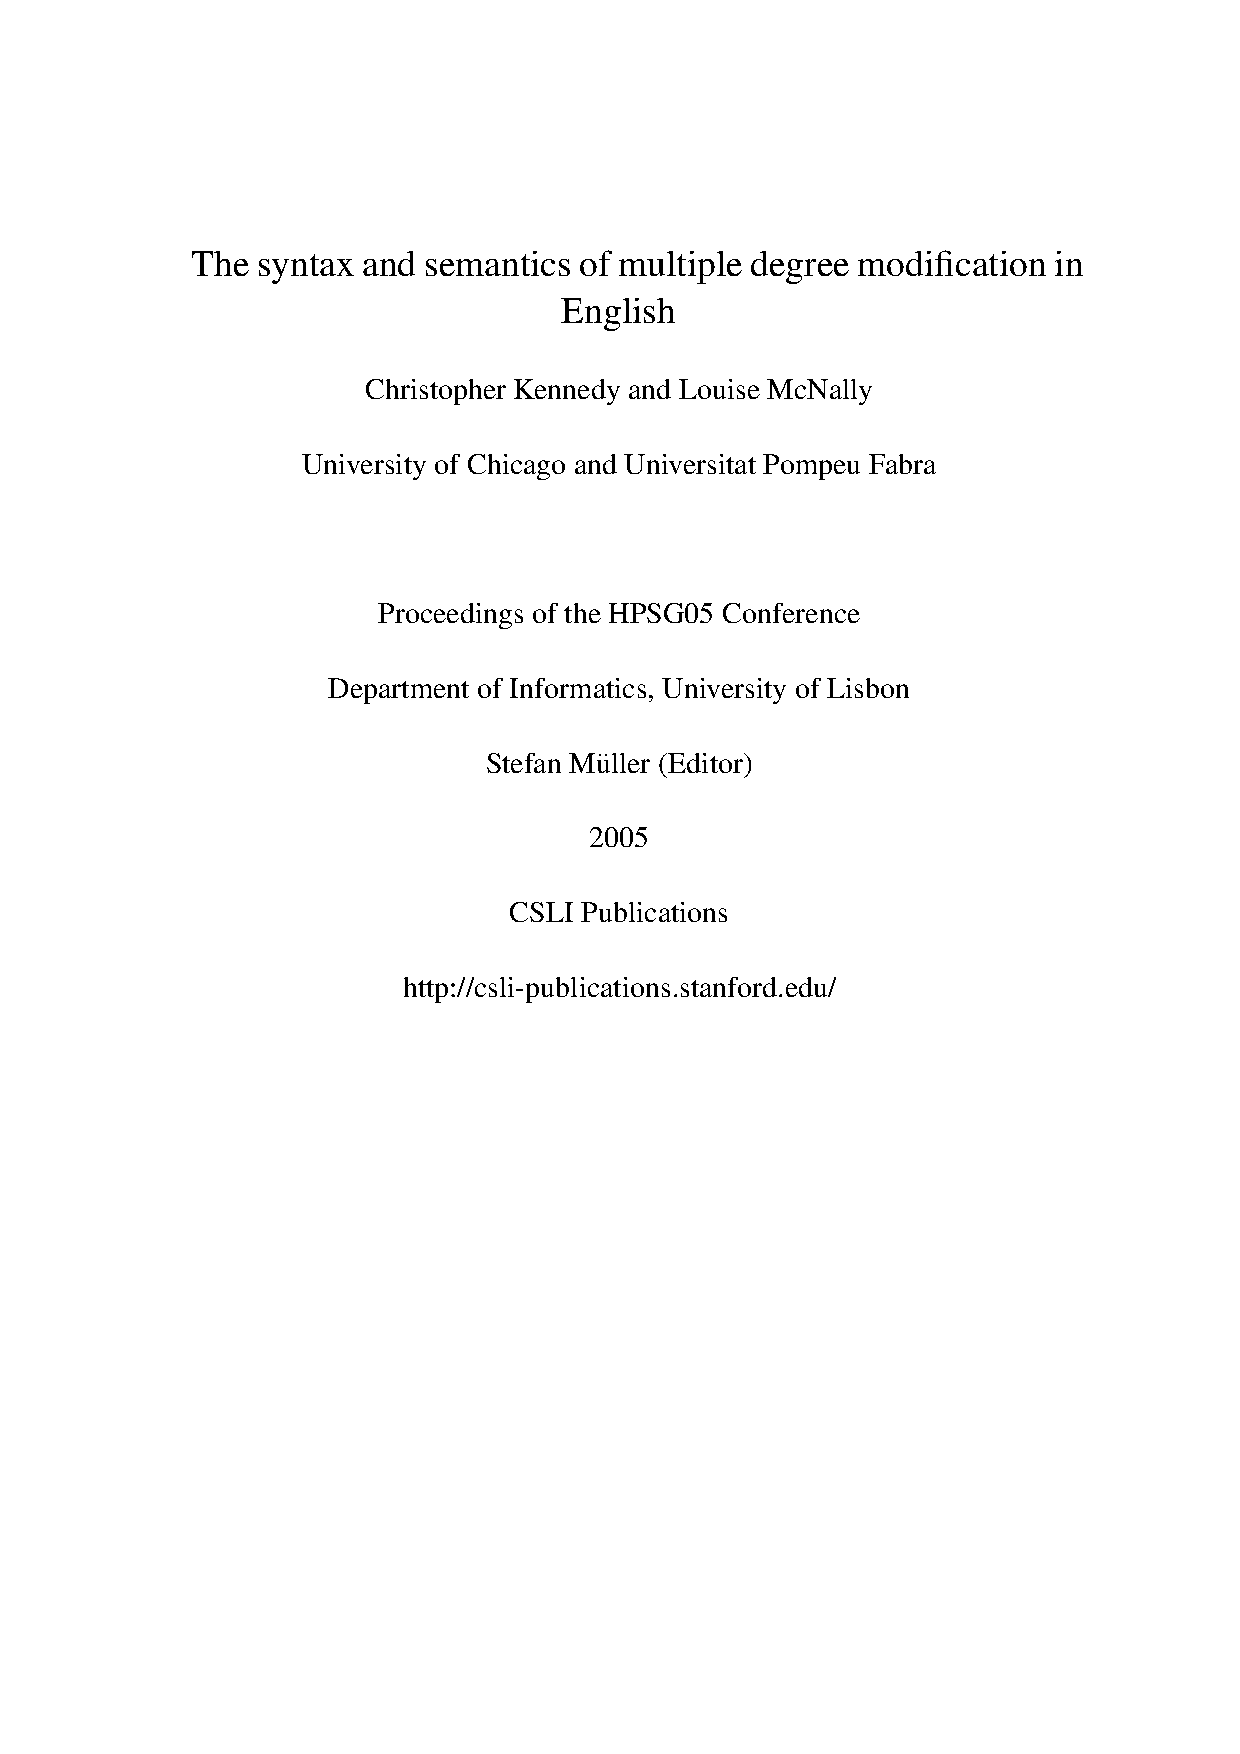
\includepdf[pages=-,pagecommand=\thispagestyle{plain},
            addtotoc={1,section,1,
            {Christopher Kennedy and Louise McNally: The Syntax and Semantics of Multiple Degree Modification in English},
             kmn}]{kennedy-mcnally.pdf}

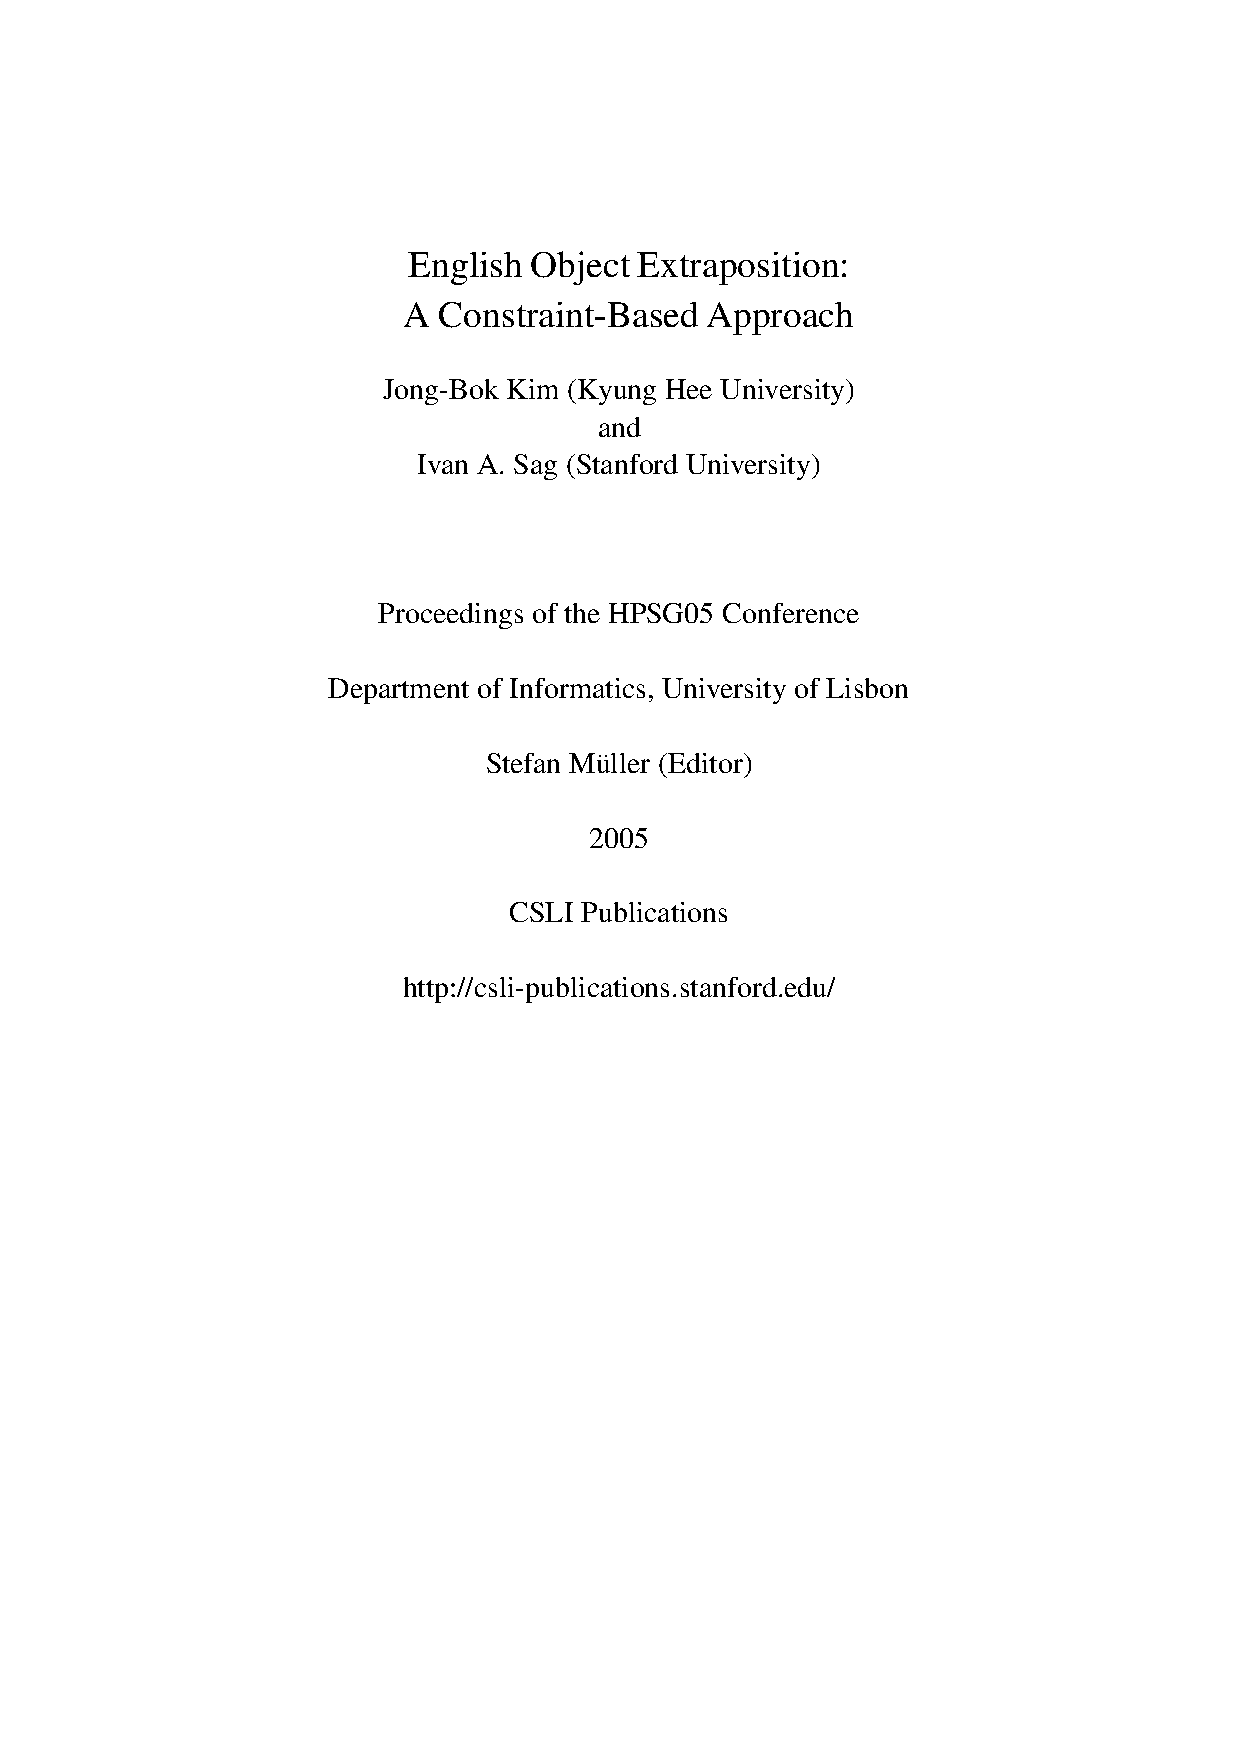
\includepdf[pages=-,pagecommand=\thispagestyle{plain},
            addtotoc={1,section,1,
            {Jong-Bok Kim and Ivan A. Sag: English Object Extraposition: A Constraint-Based Approach},
             ks}]{kim-sag.pdf}

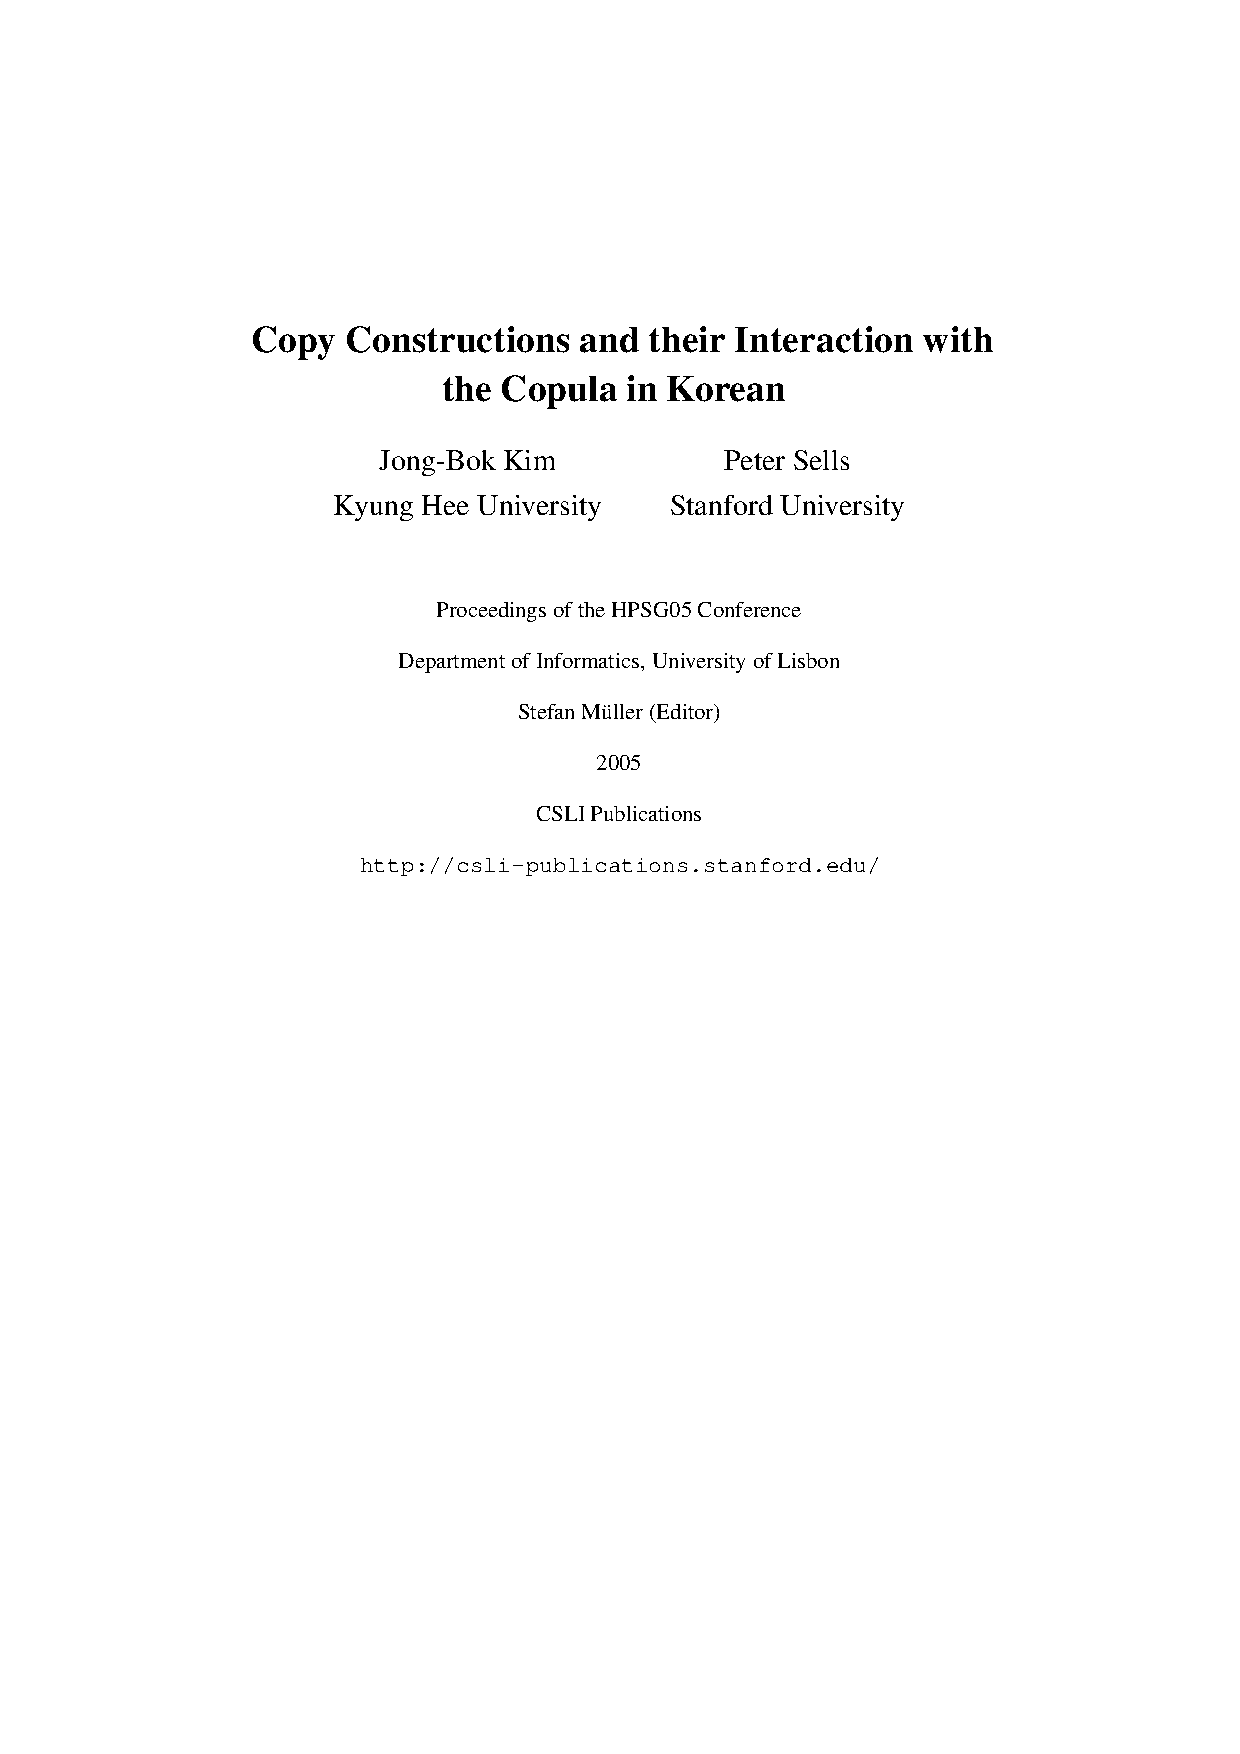
\includepdf[pages=-,pagecommand=\thispagestyle{plain},
            addtotoc={1,section,1,
            {Jong-Bok Kim and Peter Sells: Copy Constructions and their Interaction with the Copula in Korean},
             ks}]{kim-sells.pdf}


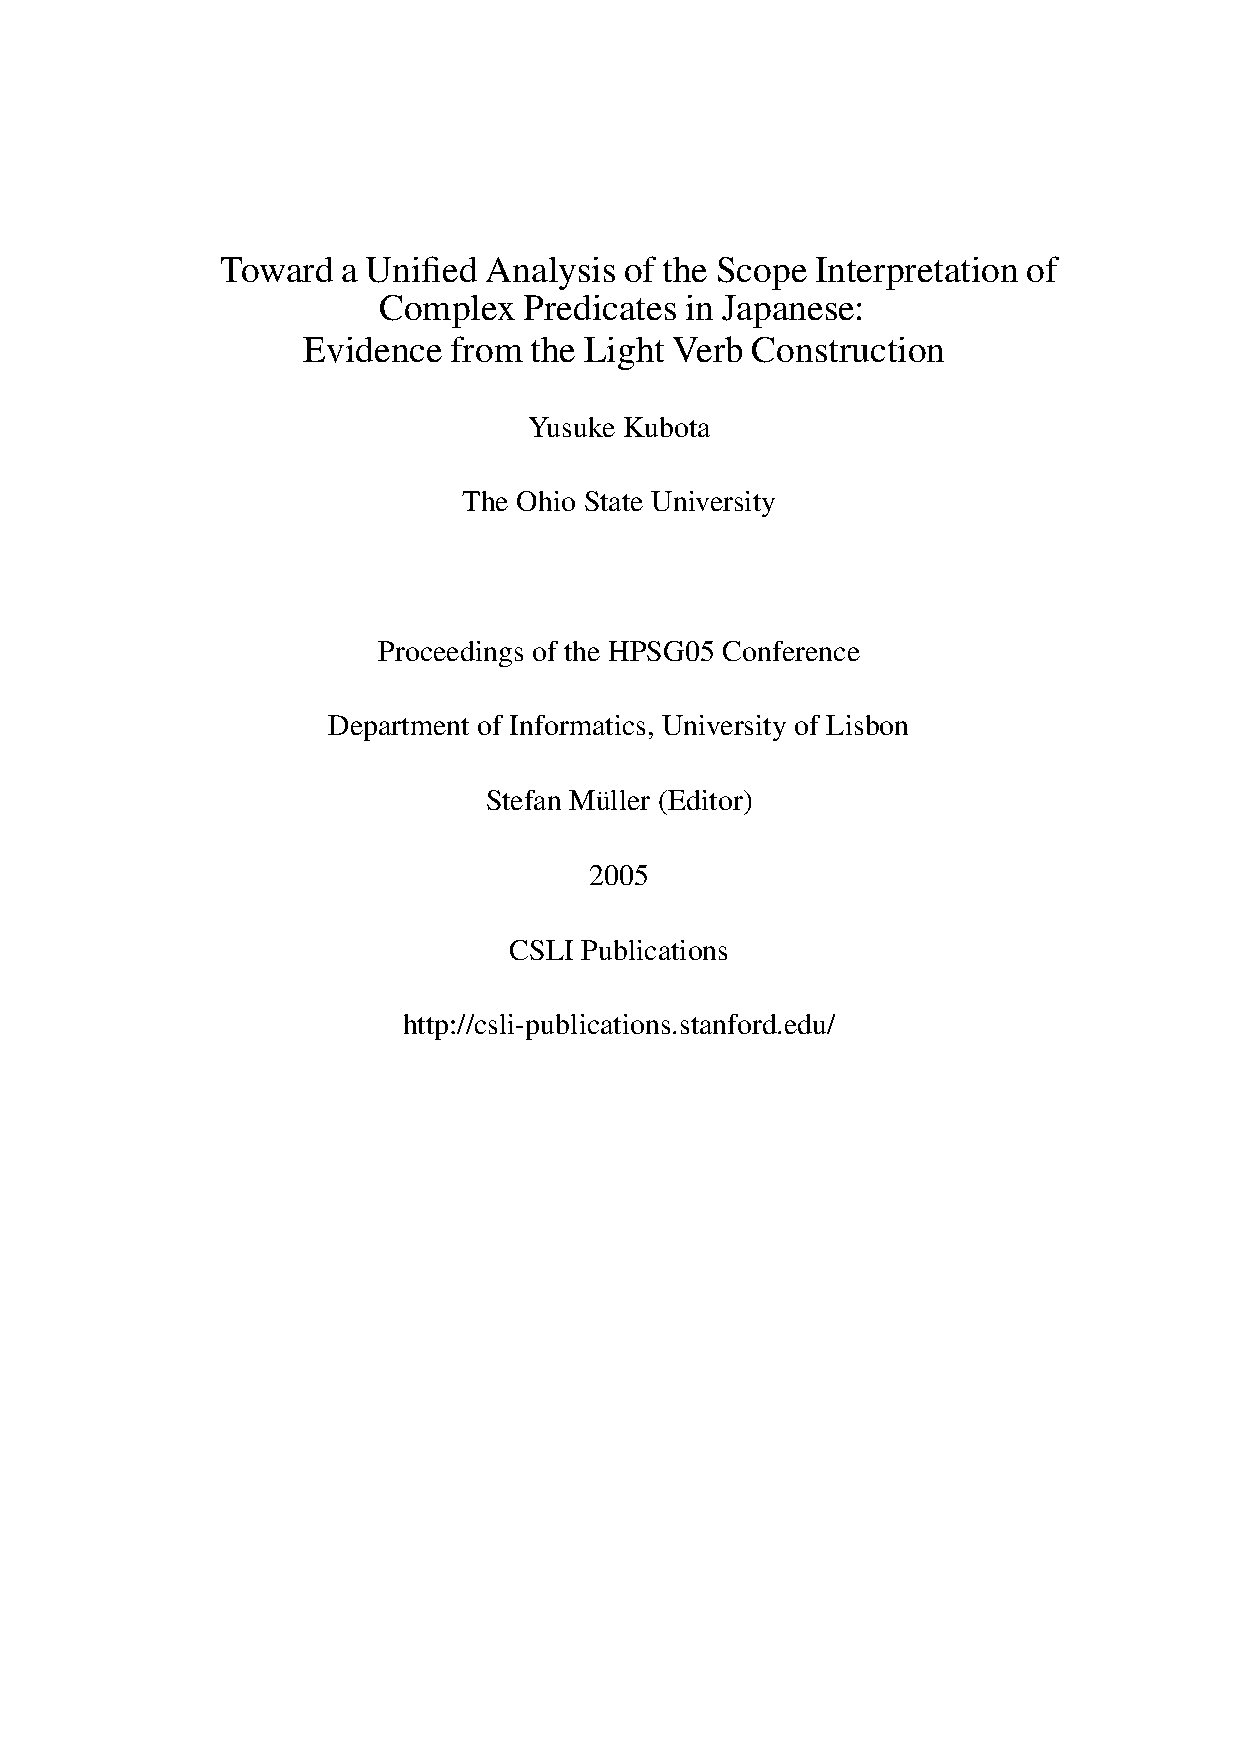
\includepdf[pages=-,pagecommand=\thispagestyle{plain},
            addtotoc={1,section,1,
            {Yusuke Kubota: Toward a Unified Analysis of the Scope Interpretation of Complex
Predicates in Japanese: Evidence from the Light Verb Construction},
             kubota}]{kubota.pdf}

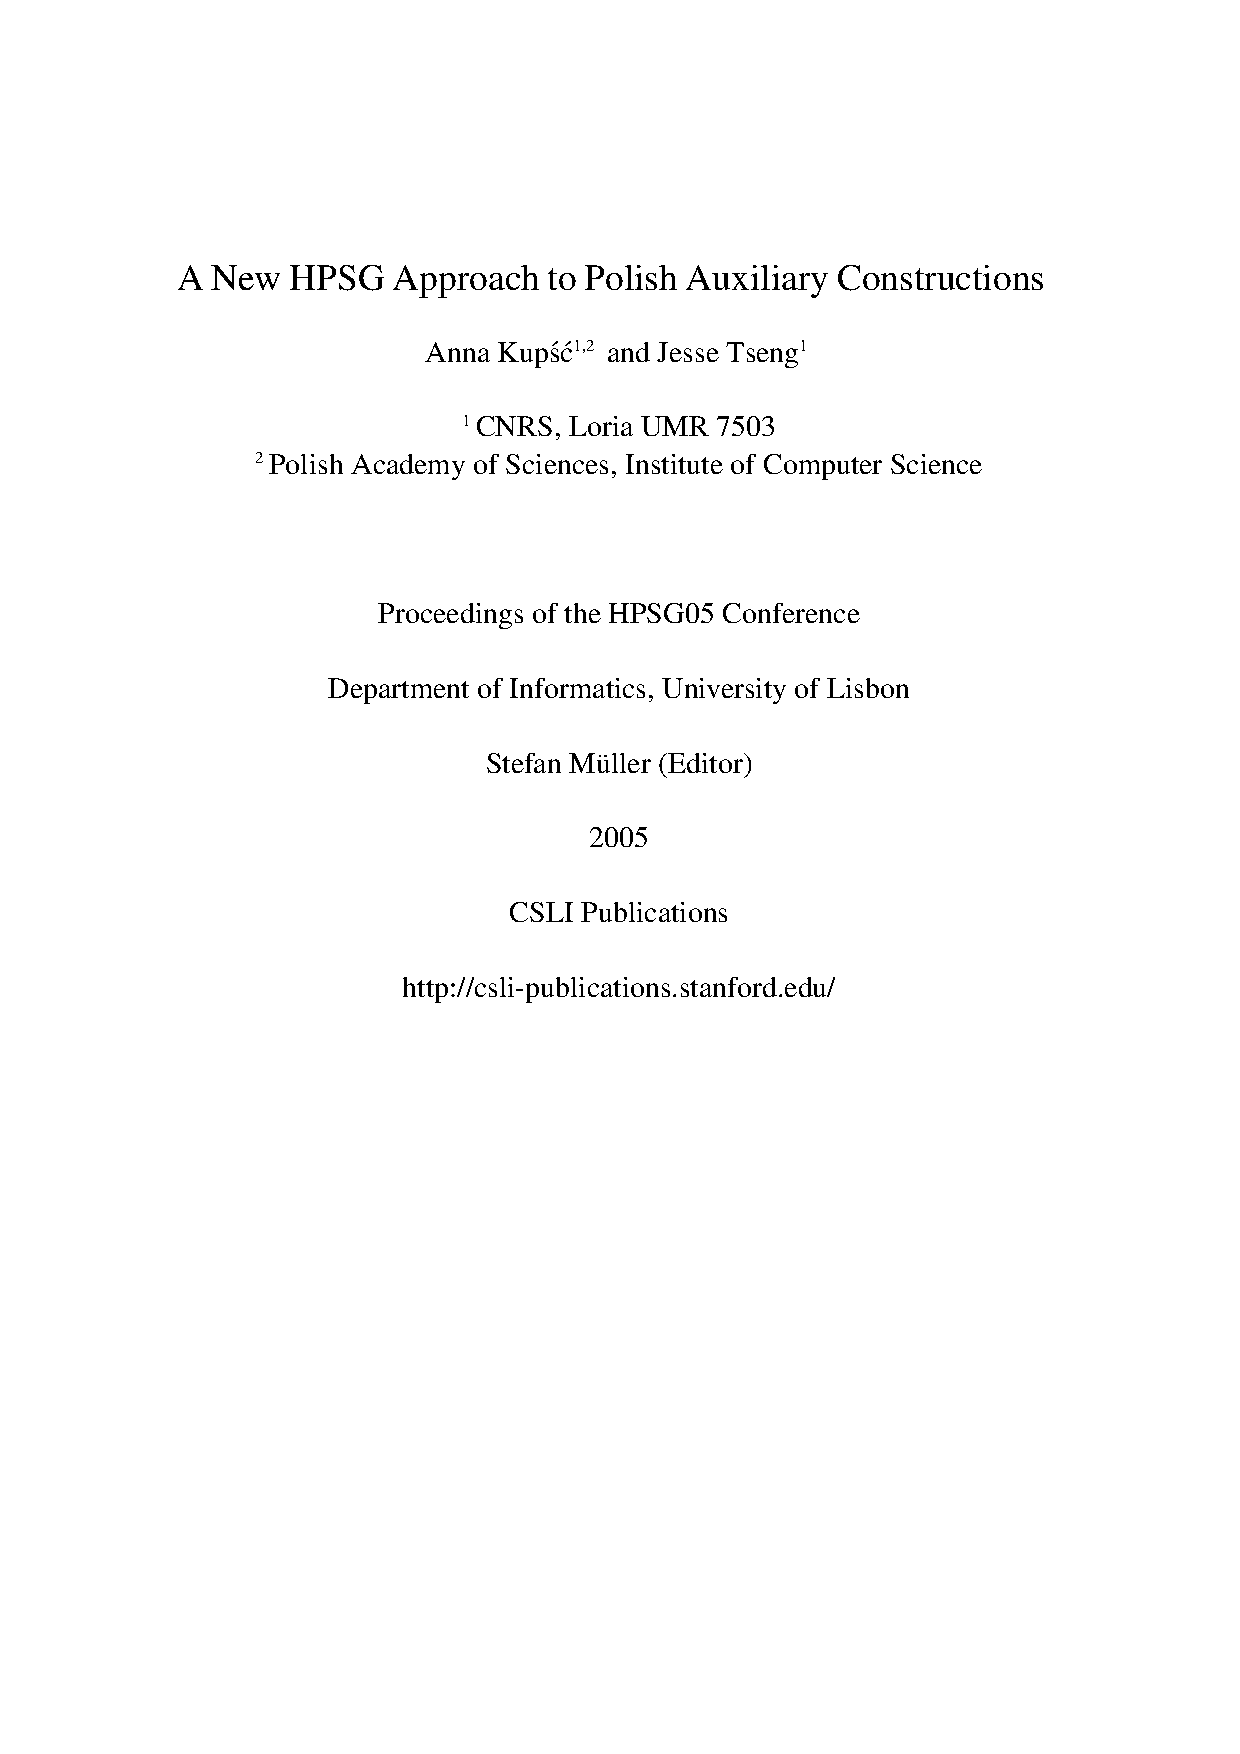
\includepdf[pages=-,pagecommand=\thispagestyle{plain},
            addtotoc={1,section,1,
            {Anna Kup{\'s}{\'c} and Jesse Tseng: A New HPSG Approach to Polish Auxiliary Constructions},
             kt}]{kupsc-tseng.pdf}

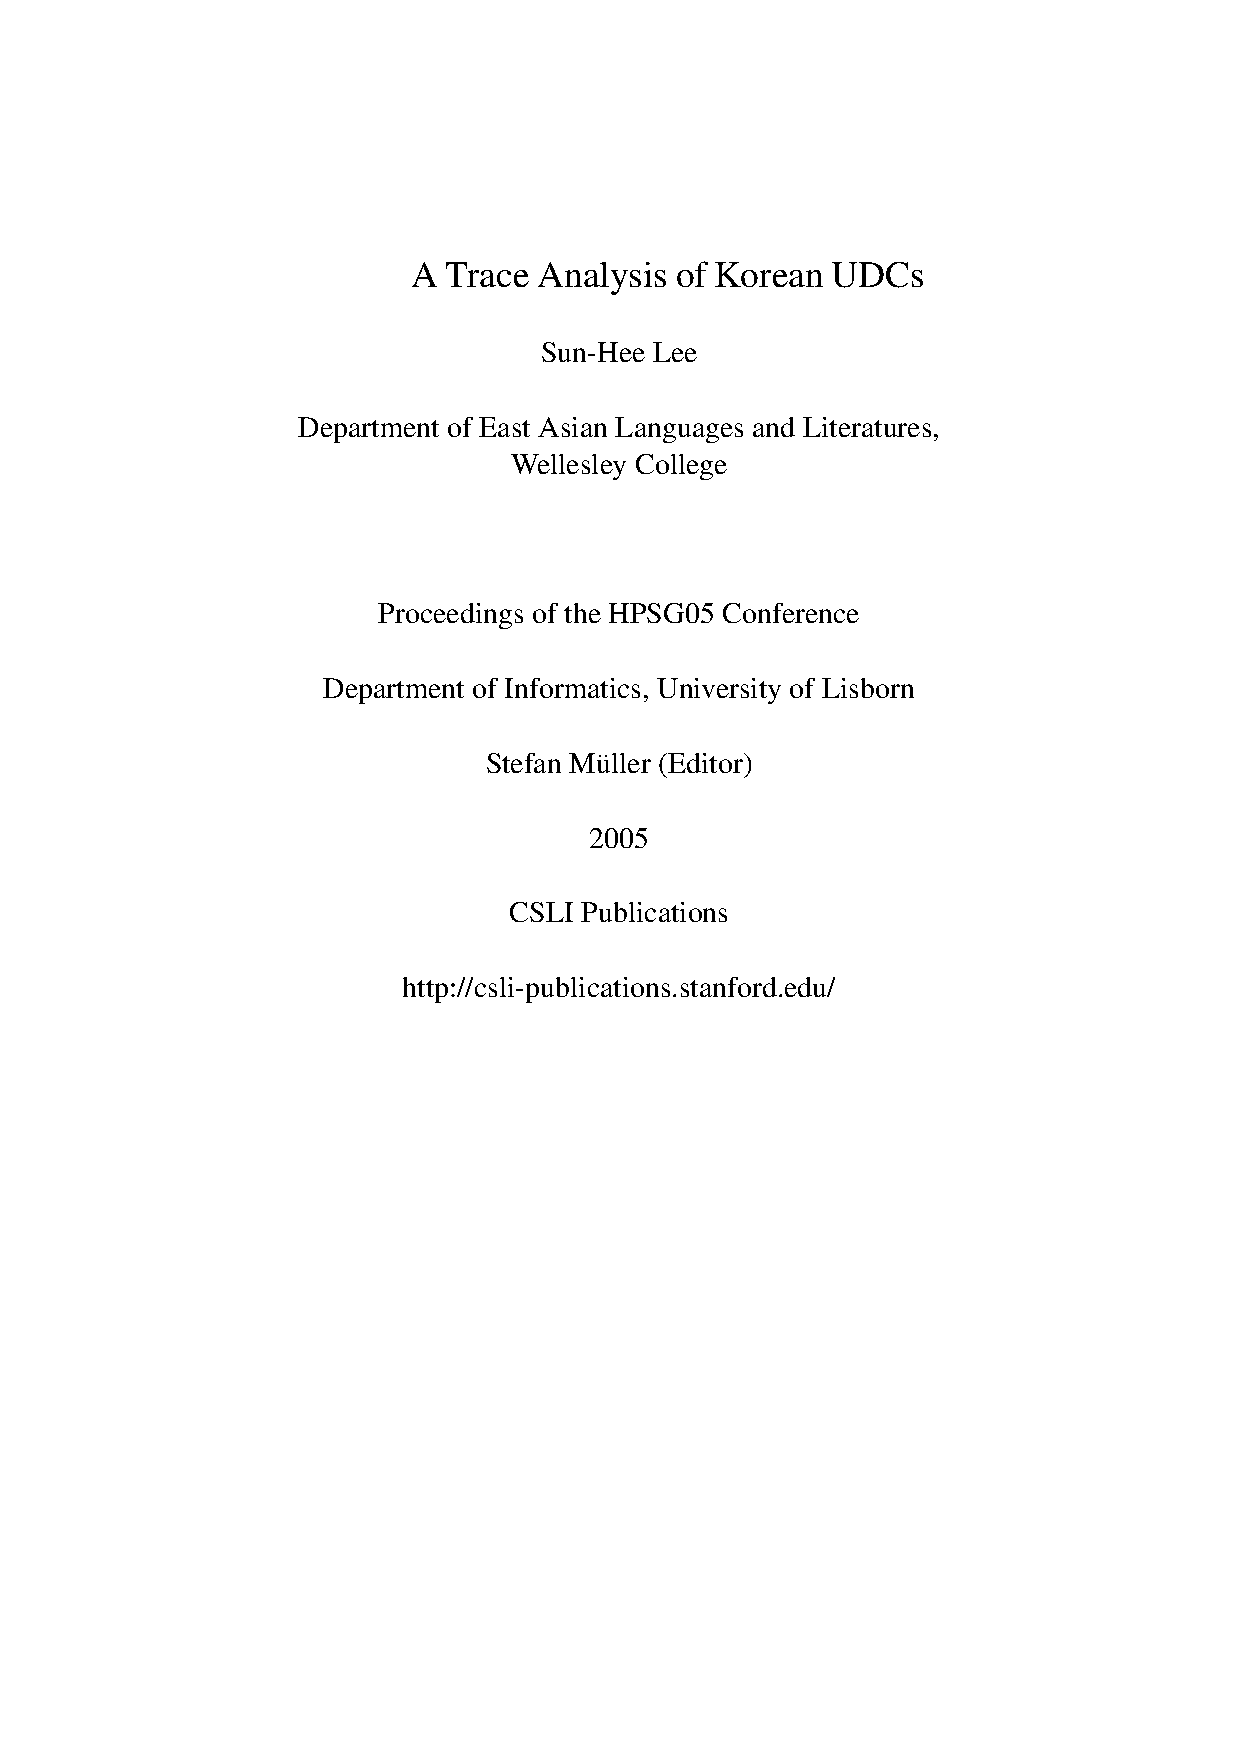
\includepdf[pages=-,pagecommand=\thispagestyle{plain},
            addtotoc={1,section,1,
            {Sun-Hee Lee: A Trace Analysis of Korean UDCs},
             lee}]{lee.pdf}


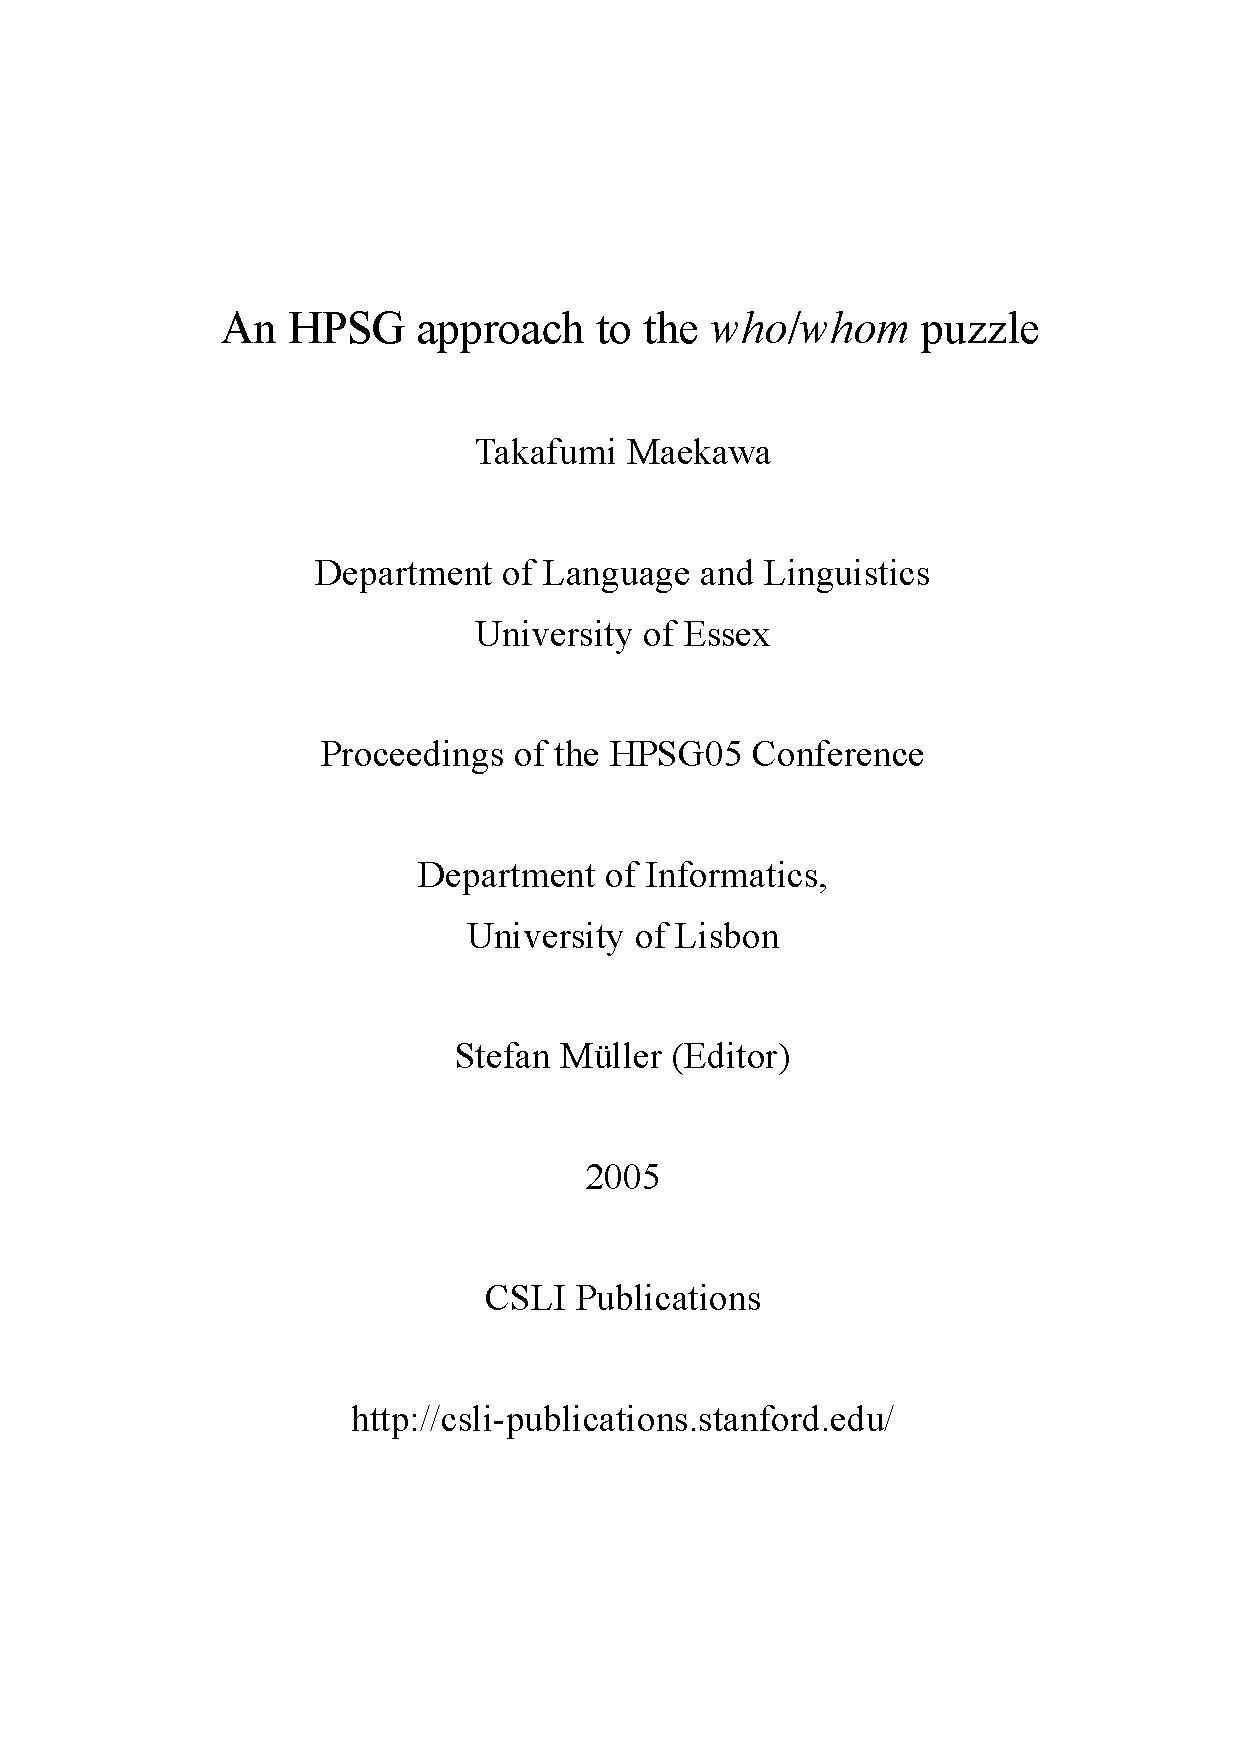
\includepdf[pages=-,pagecommand=\thispagestyle{plain},
            addtotoc={1,section,1,
            {Takafumi Maekawa: An HPSG Approach to the <em>who</em>/<em>whom</em> Puzzle},
             maekawa}]{maekawa.pdf}

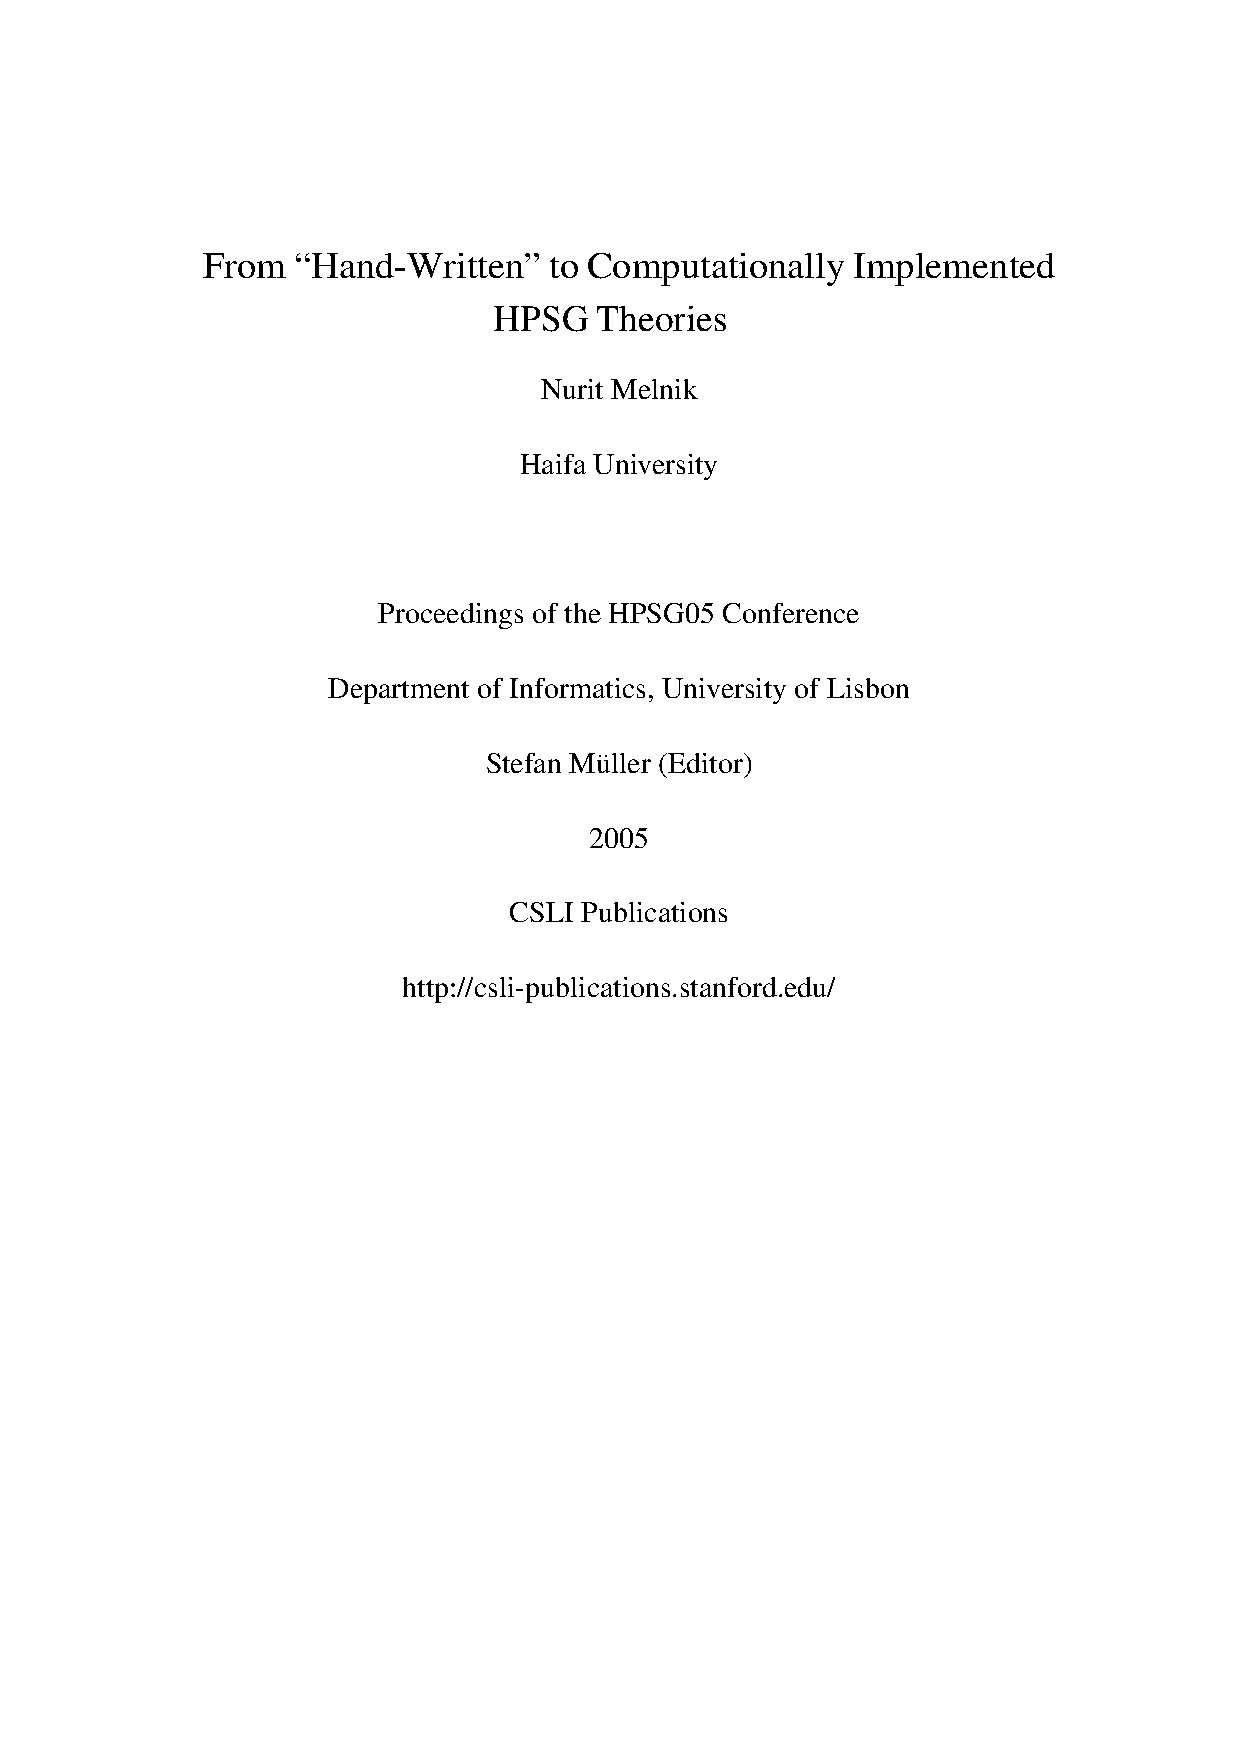
\includepdf[pages=-,pagecommand=\thispagestyle{plain},
            addtotoc={1,section,1,
            {Nurit Melnik: From ``hand-written'' to Computationally Implemented HPSG Theories},
             melnik}]{melnik.pdf}

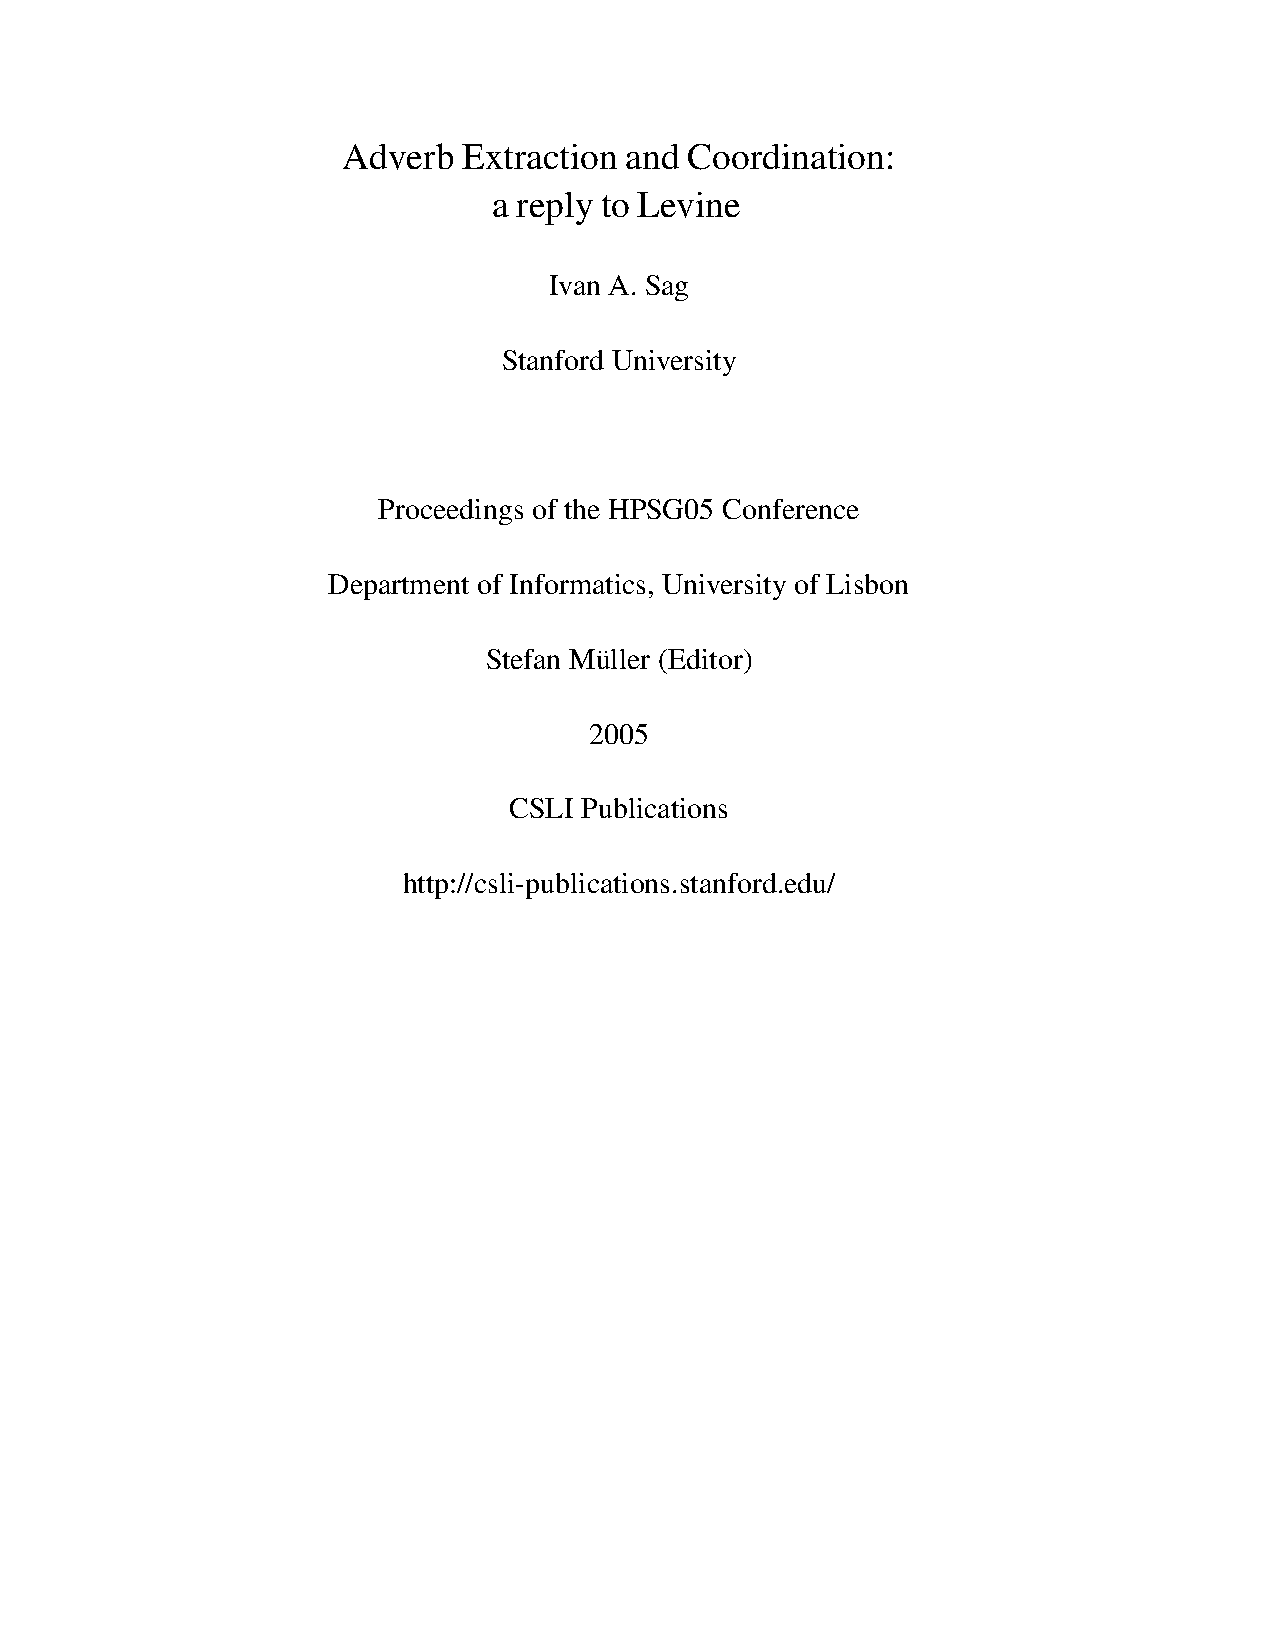
\includepdf[pages=-,pagecommand=\thispagestyle{plain},
            addtotoc={1,section,1,
            {Ivan A. Sag: Adverb Extraction and Coordination: a Reply to Levine},
             sag}]{sag.pdf}

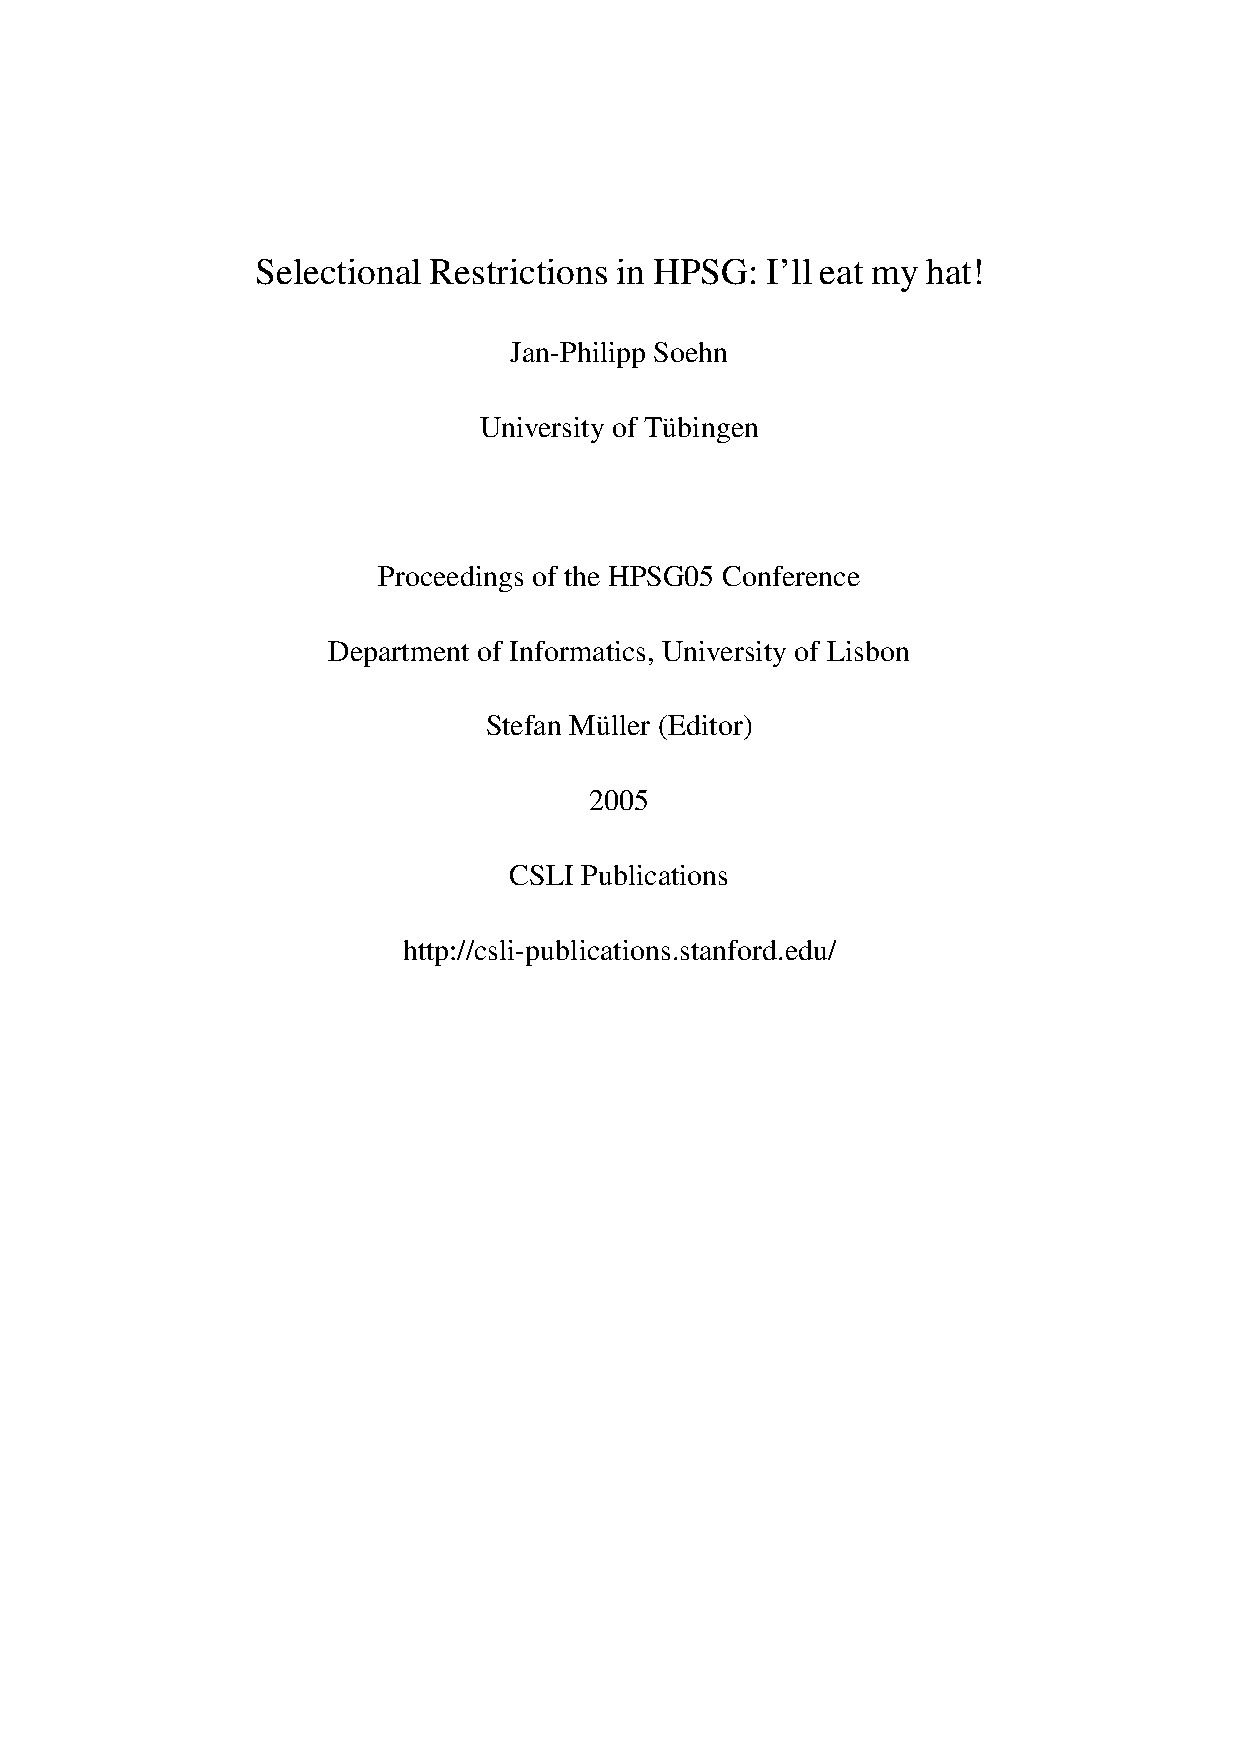
\includepdf[pages=-,pagecommand=\thispagestyle{plain},
            addtotoc={1,section,1,
            {Jan-Philipp Soehn: Selectional Restrictions in HPSG: I'll eat my hat!},
             soehn}]{soehn.pdf}

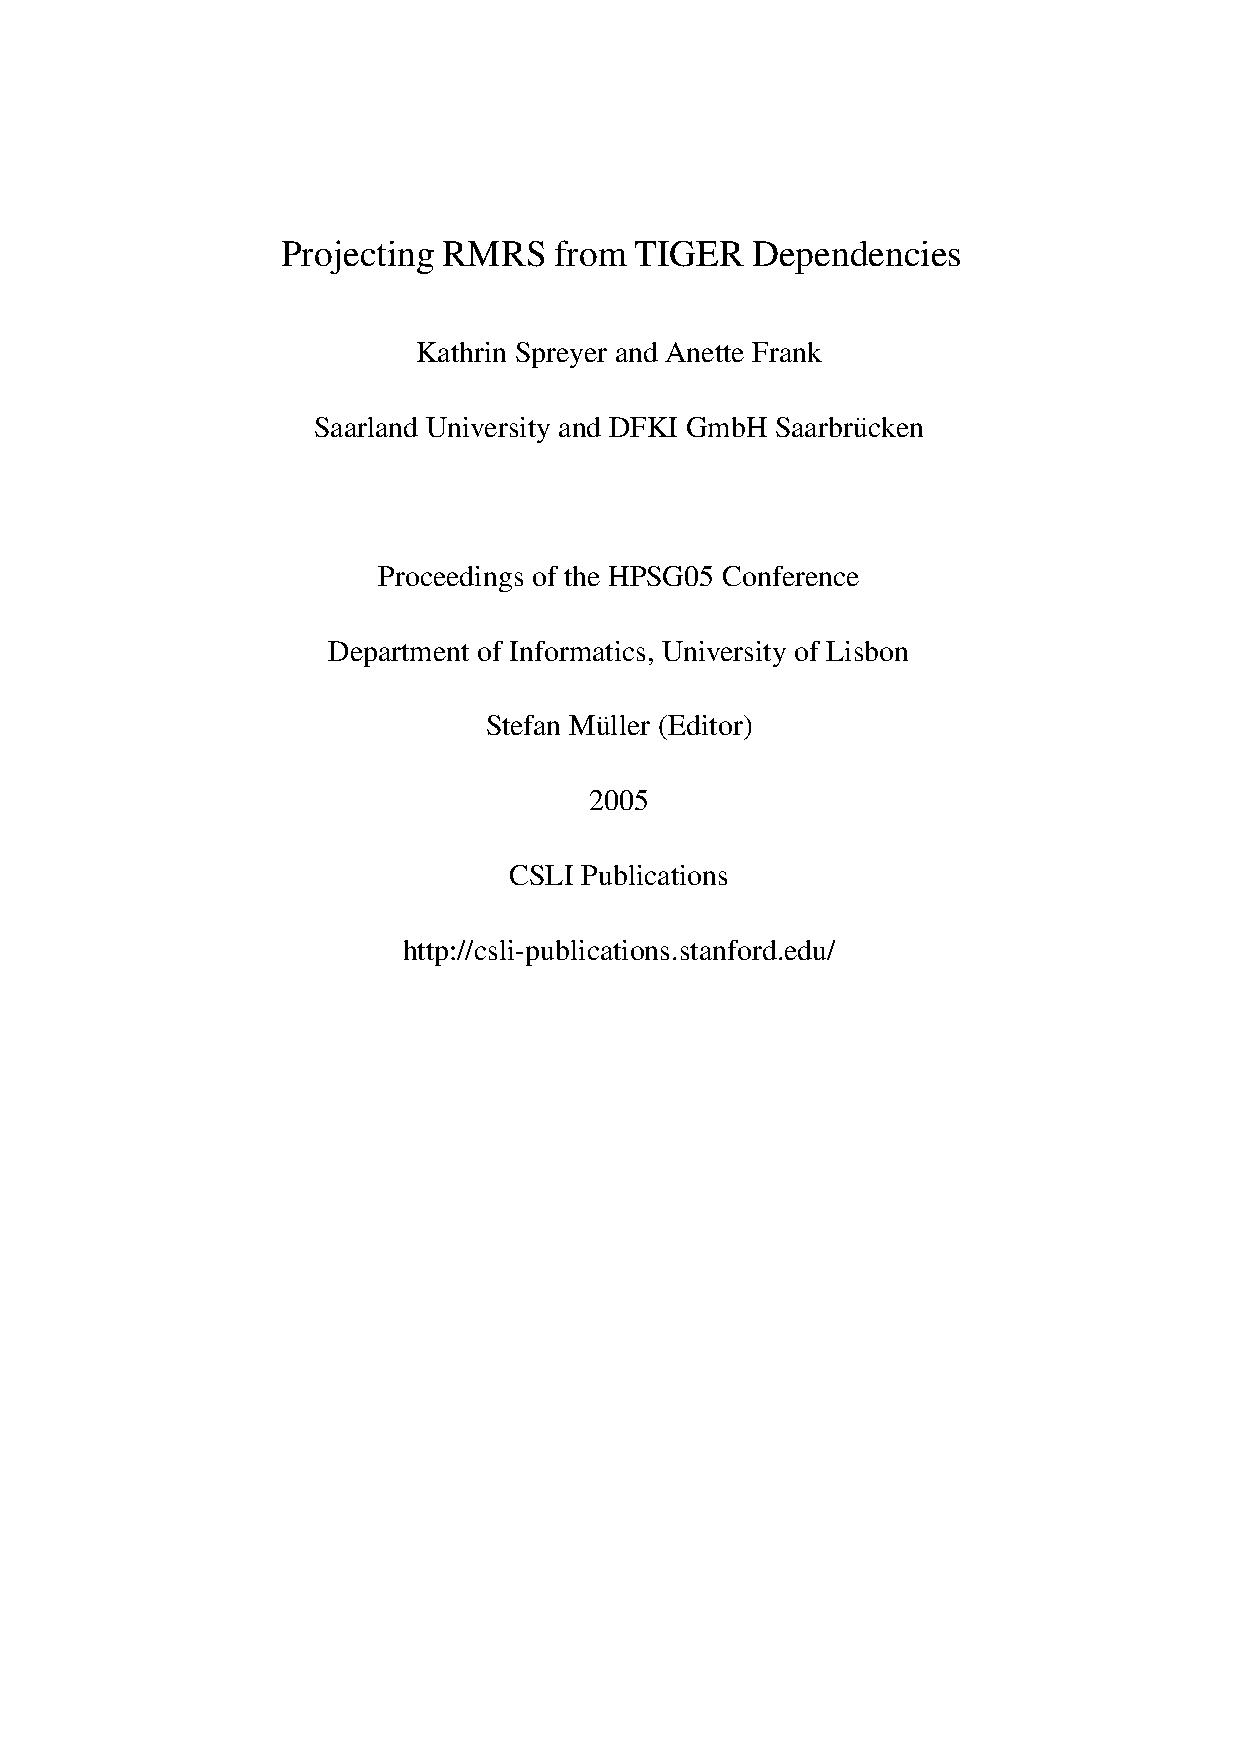
\includepdf[pages=-,pagecommand=\thispagestyle{plain},
            addtotoc={1,section,1,
            {Kathrin Spreyer and Anette Frank: Projecting RMRS from TIGER Dependencies},
             spreyer-frank}]{spreyer-frank.pdf}

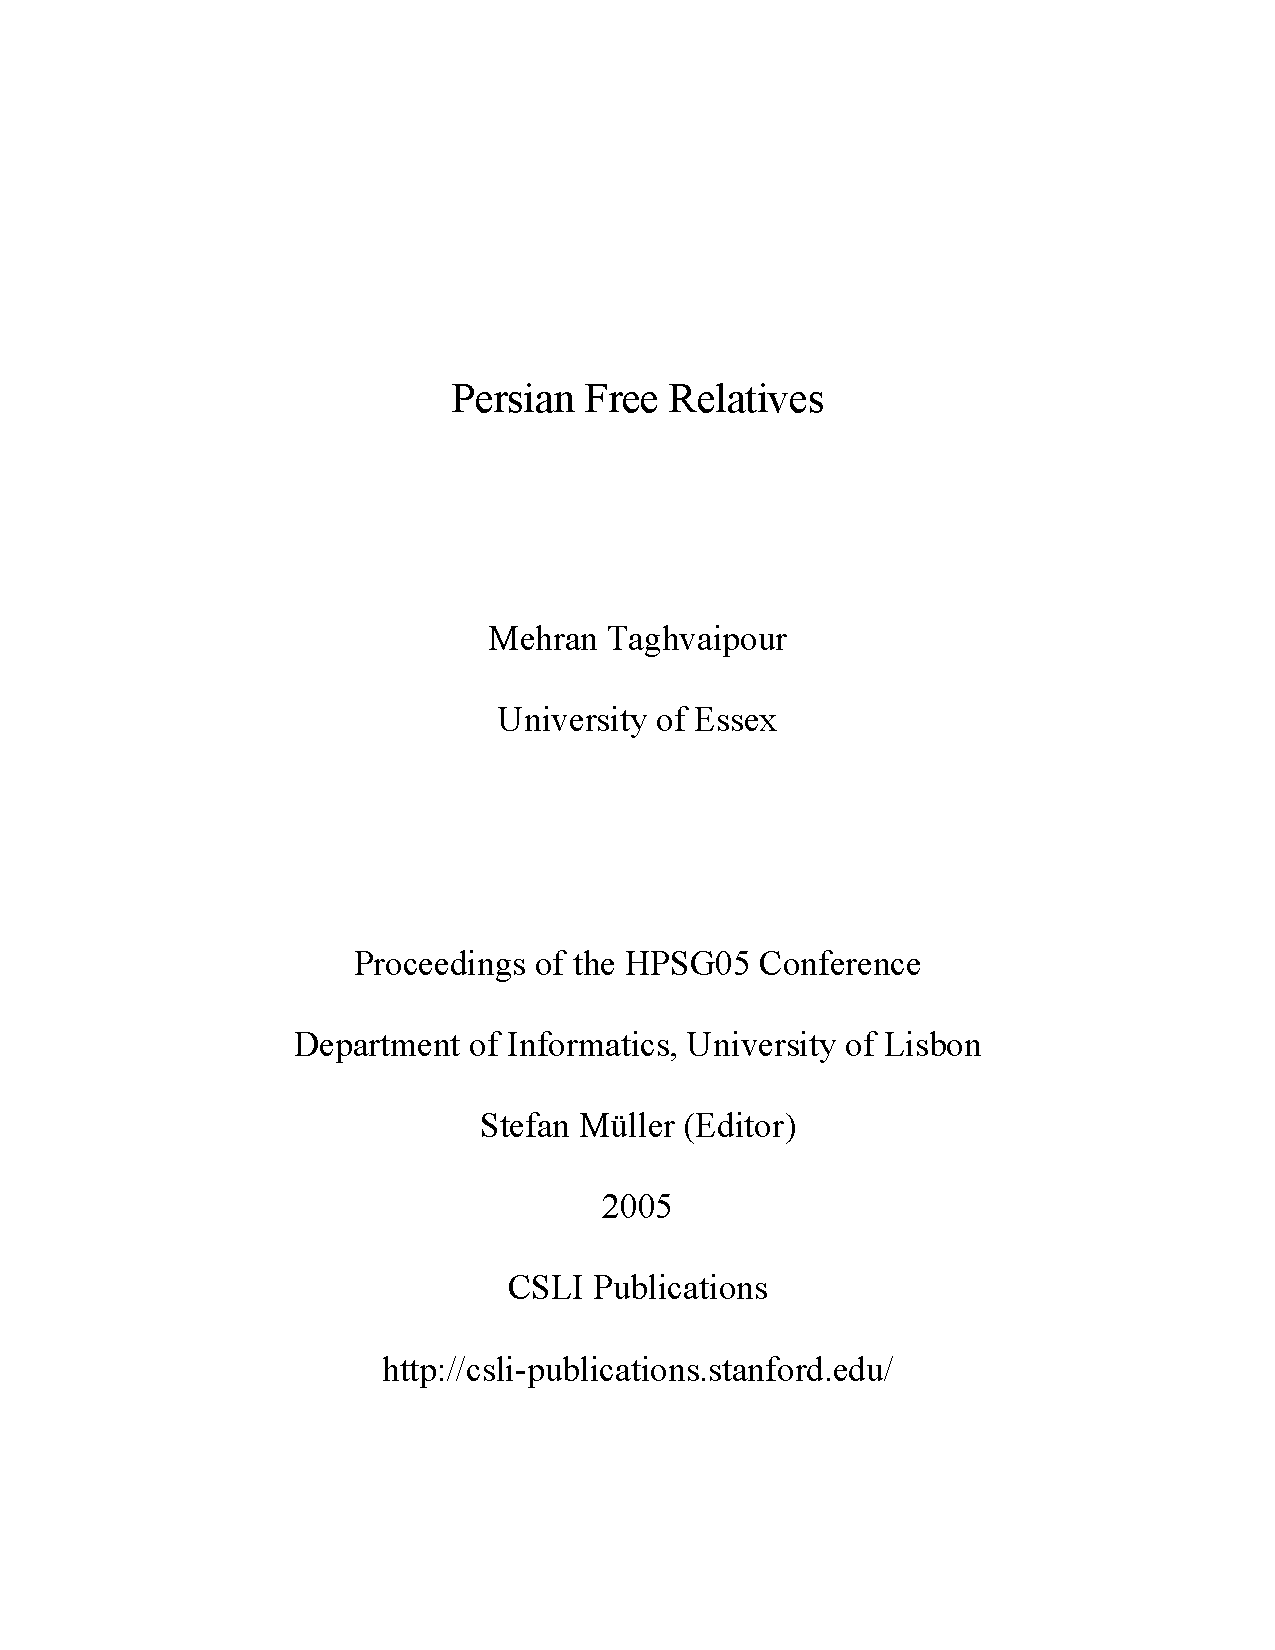
\includepdf[pages=-,pagecommand=\thispagestyle{plain},
            addtotoc={1,section,1,
            {Mehran A Taghvaipour: Persian Free Relatives},
             taghvaipour}]{taghvaipour.pdf}


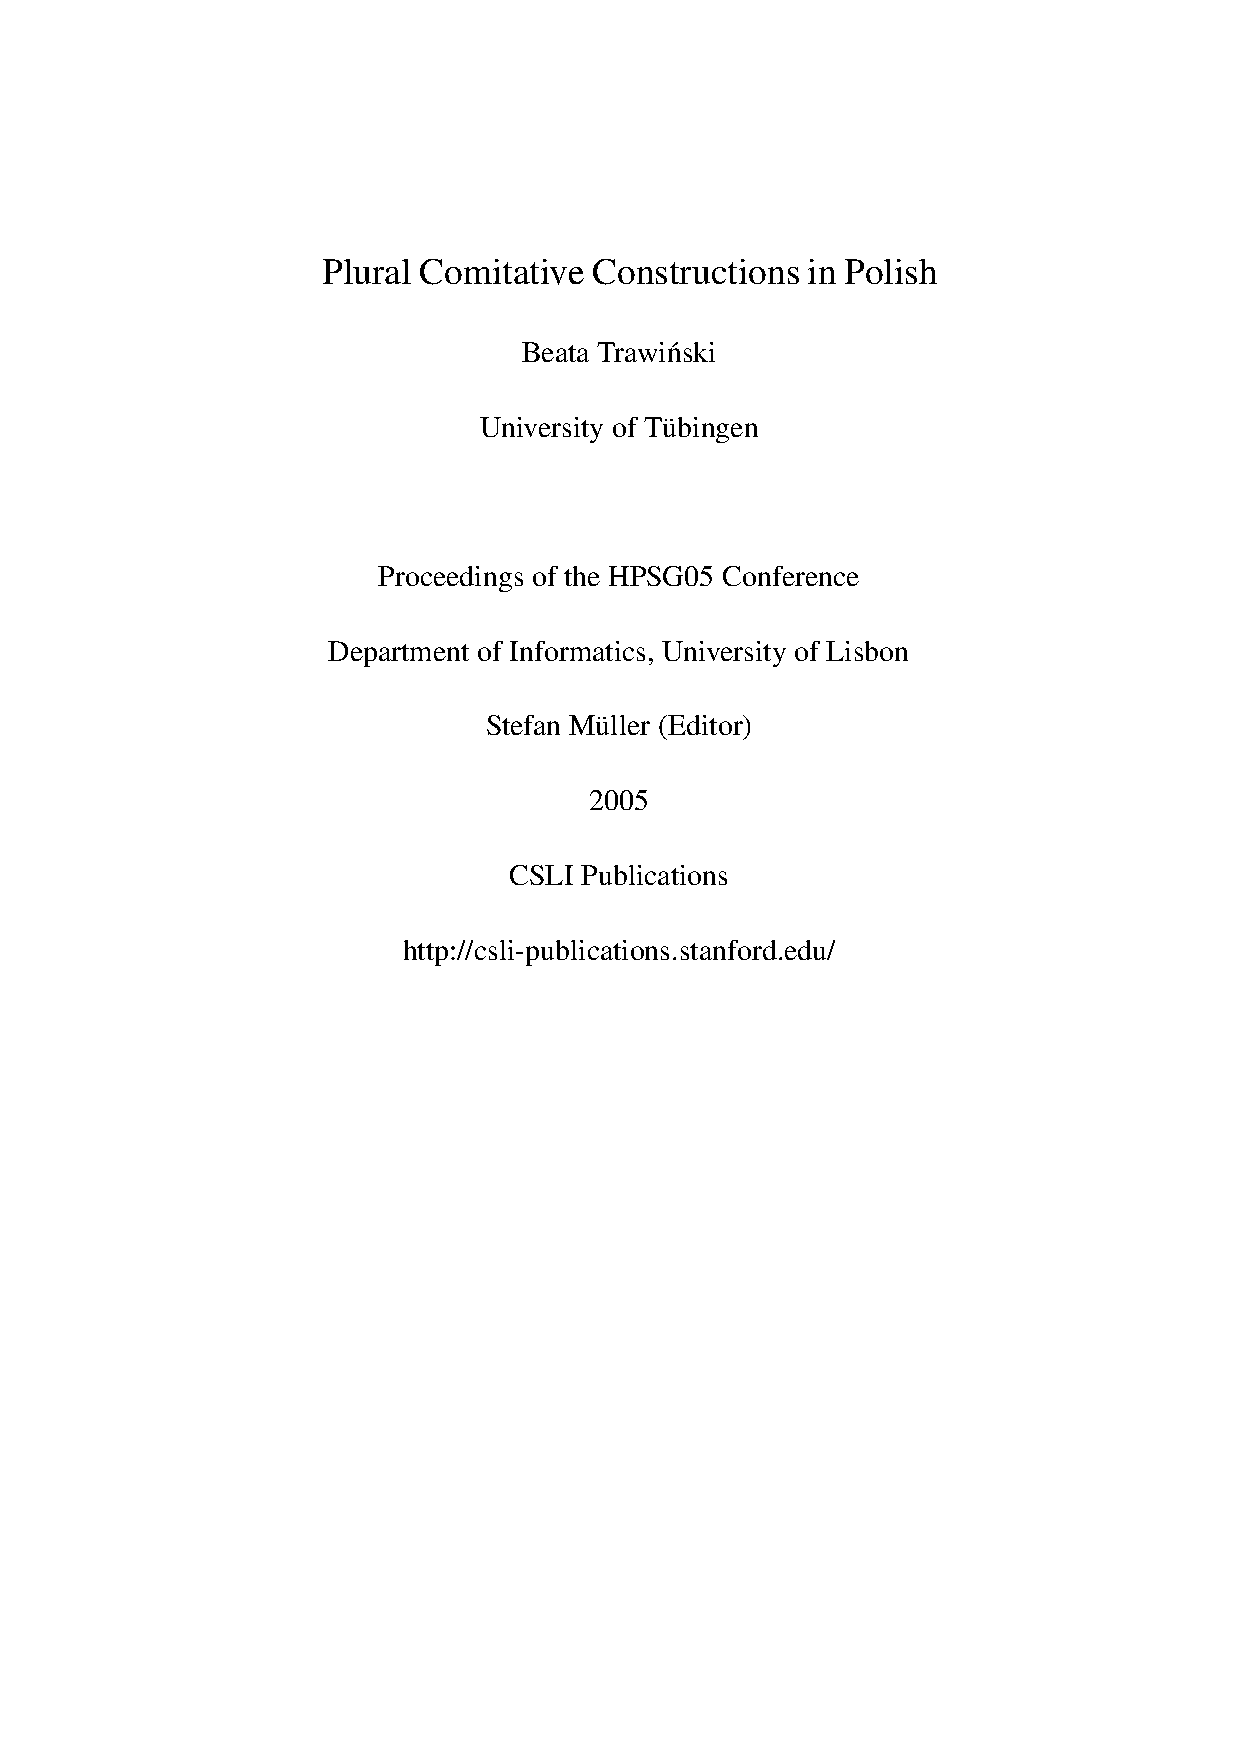
\includepdf[pages=-,pagecommand=\thispagestyle{plain},
            addtotoc={1,section,1,
            {Beata Trawinski: Plural Comitative Constructions in Polish},
             trawinski}]{trawinski.pdf}



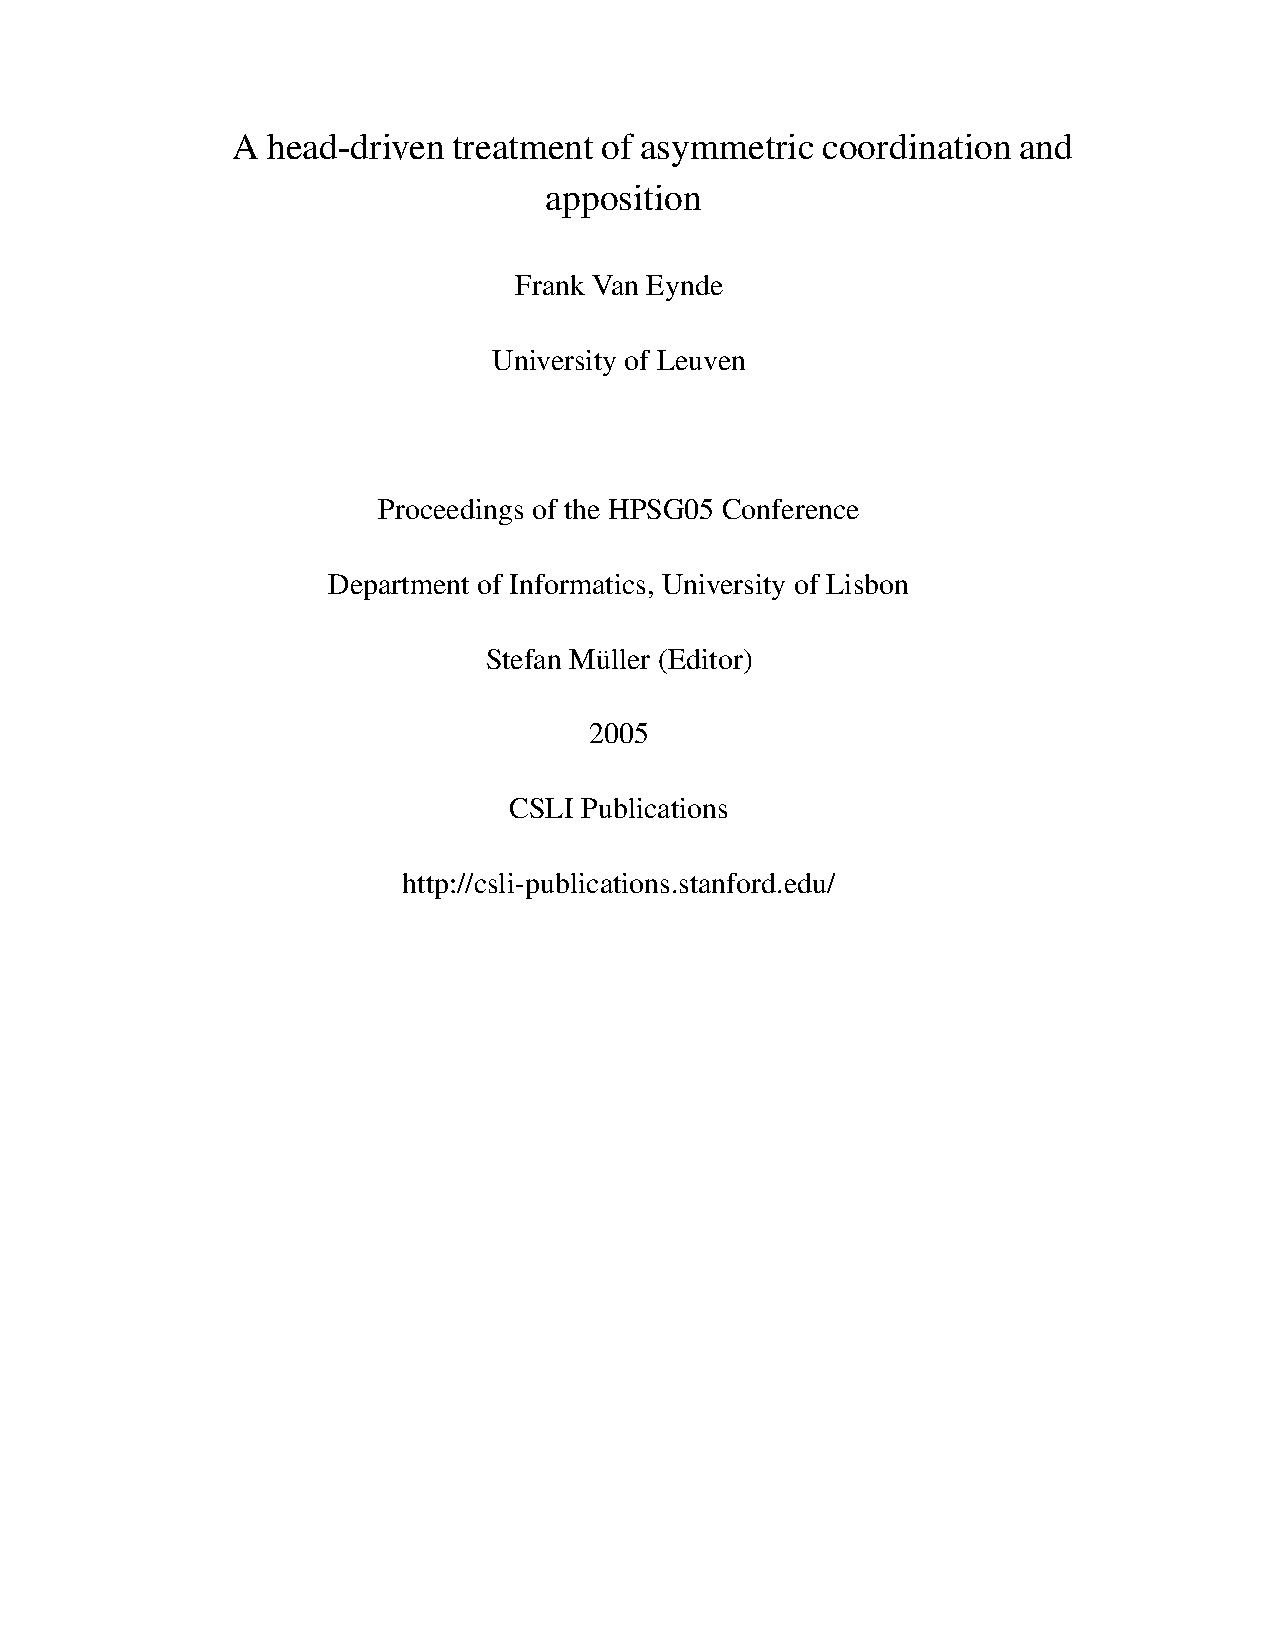
\includepdf[pages=-,pagecommand=\thispagestyle{plain},
            addtotoc={1,section,1,
            {Frank Van Eynde: A Head-Driven Treatment of Asymmetric Coordination and Apposition},
             vaneynde}]{vaneynde.pdf}

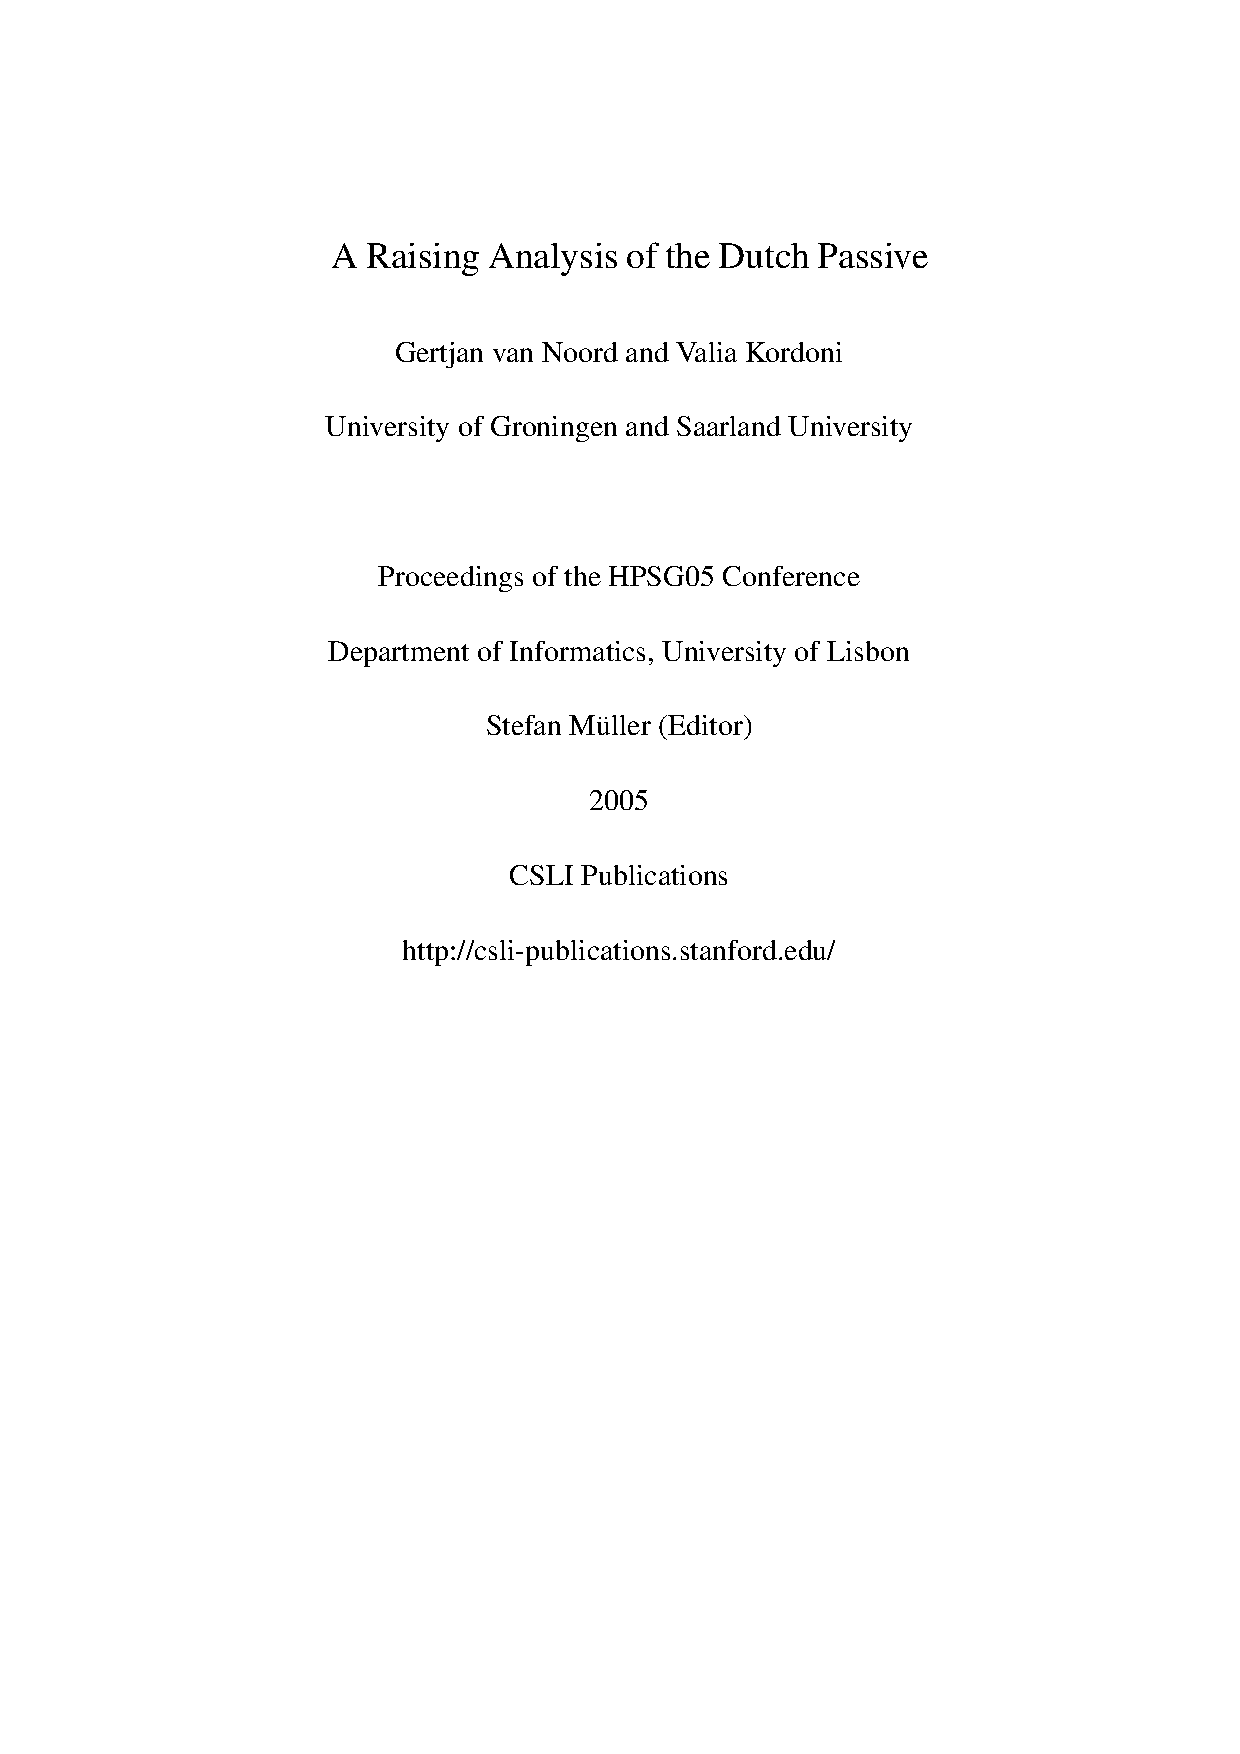
\includepdf[pages=-,pagecommand=\thispagestyle{plain},
            addtotoc={1,section,1,
            {Gertjan van Noord and Valia Kordoni: A Raising Analysis of the Dutch Passive},
             vnk}]{vannoord-kordoni.pdf}

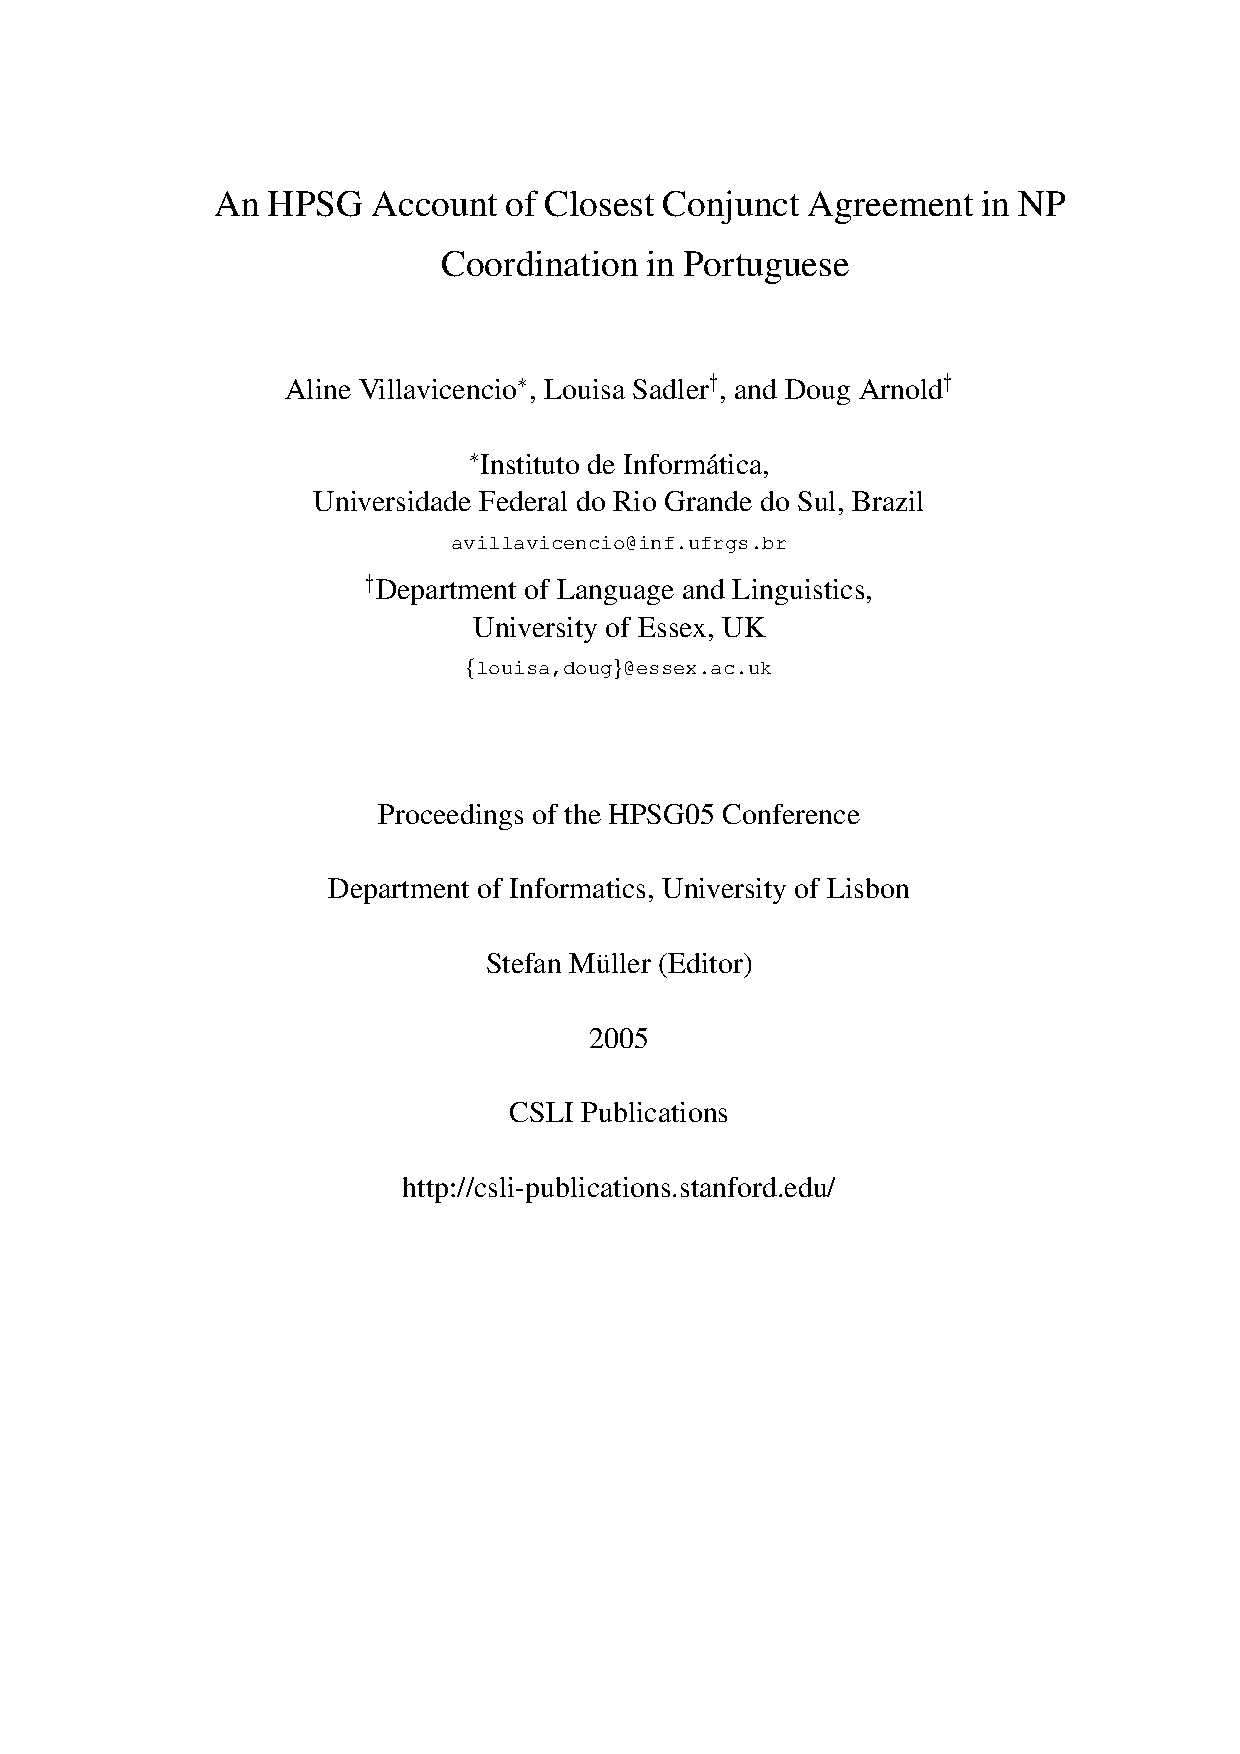
\includepdf[pages=-,pagecommand=\thispagestyle{plain},
            addtotoc={1,section,1,
            {Aline Villavicencio, Louisa Sadler, and Doug Arnold: An HPSG Account of Closest Conjunct Agreement in NP Coordination in Portuguese},
             vsa}]{vsa.pdf}

\newpage
\part{Contributions to the Workshop on \emph{Binding Theory and Invariants in Anaphoric Relations}}




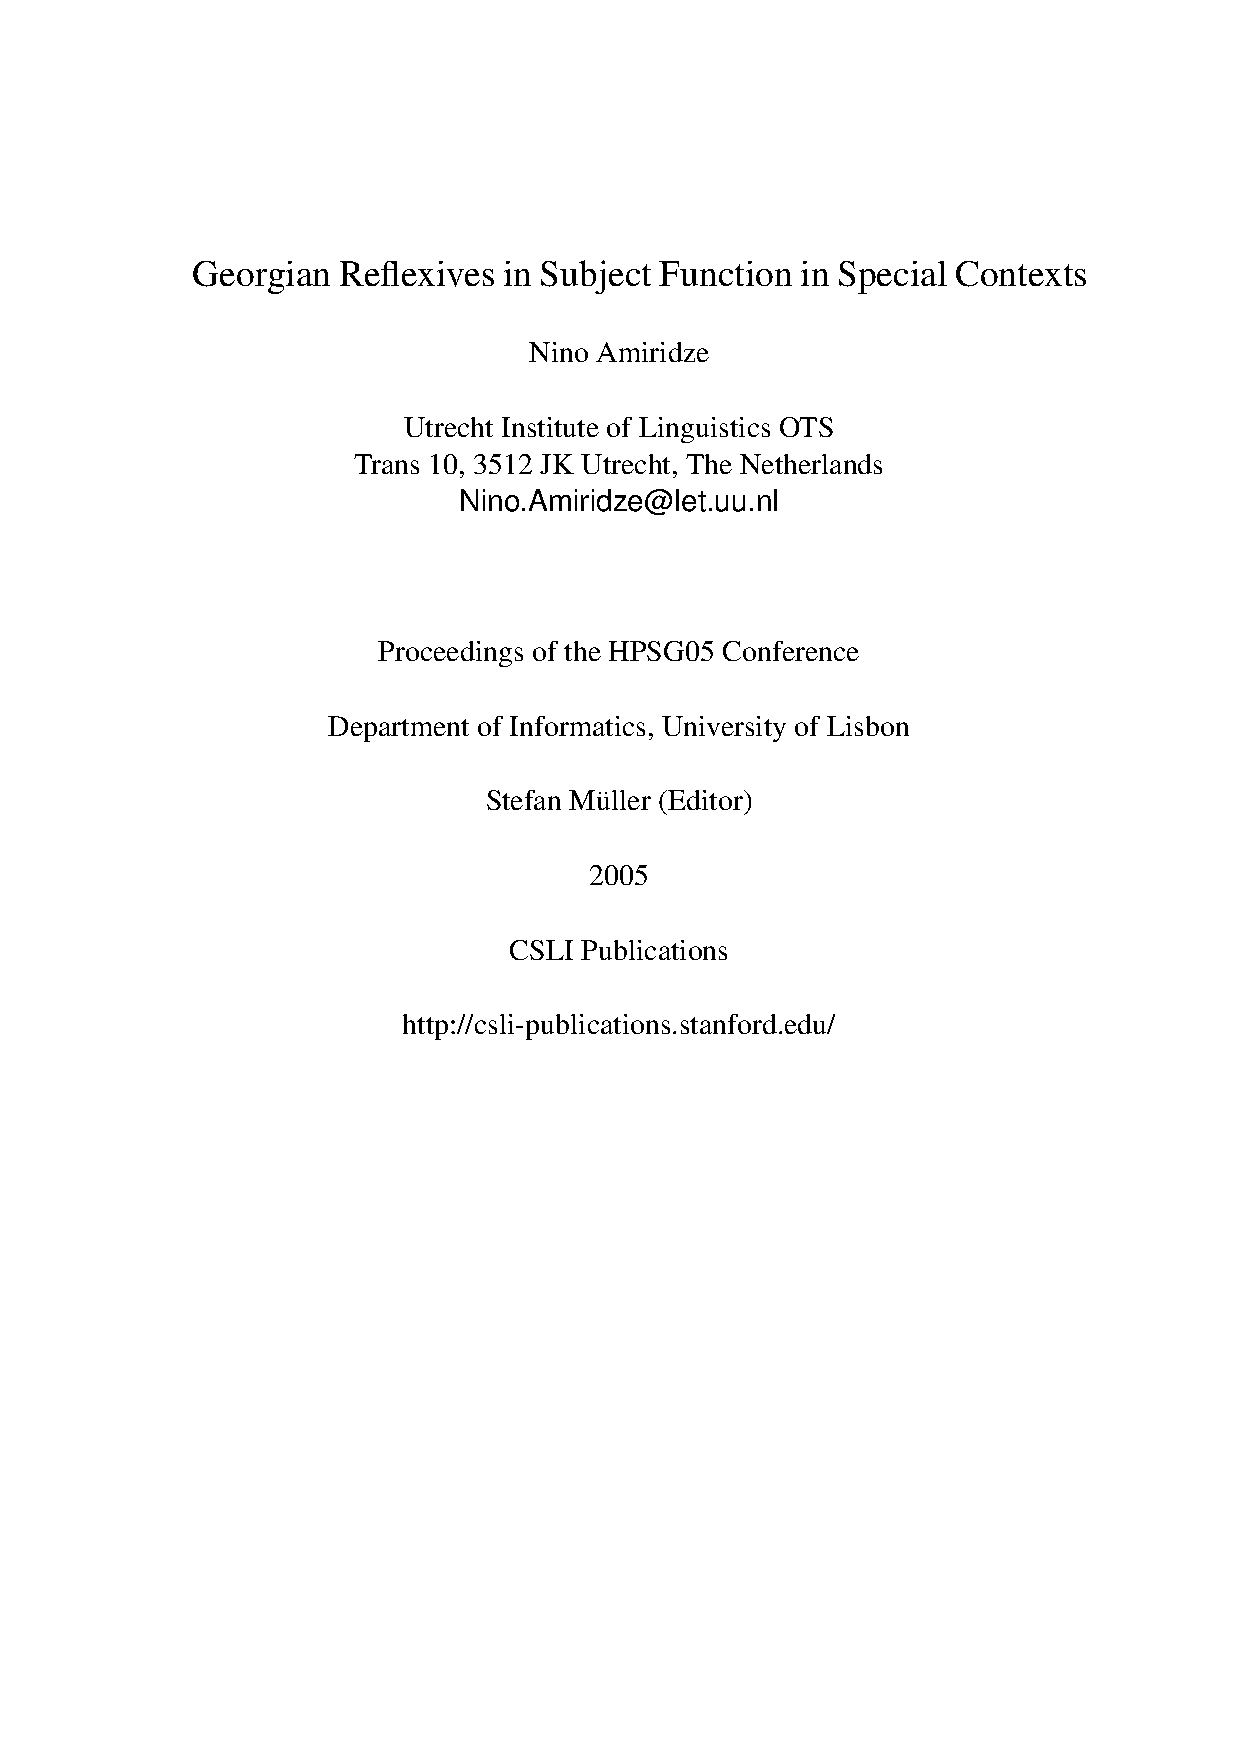
\includepdf[pages=-,pagecommand=\thispagestyle{plain},
            addtotoc={1,section,1,
            {Nino Amiridze: Georgian Reflexives in Subject Function in Special Contexts},
             amiridze}]{amiridze.pdf}


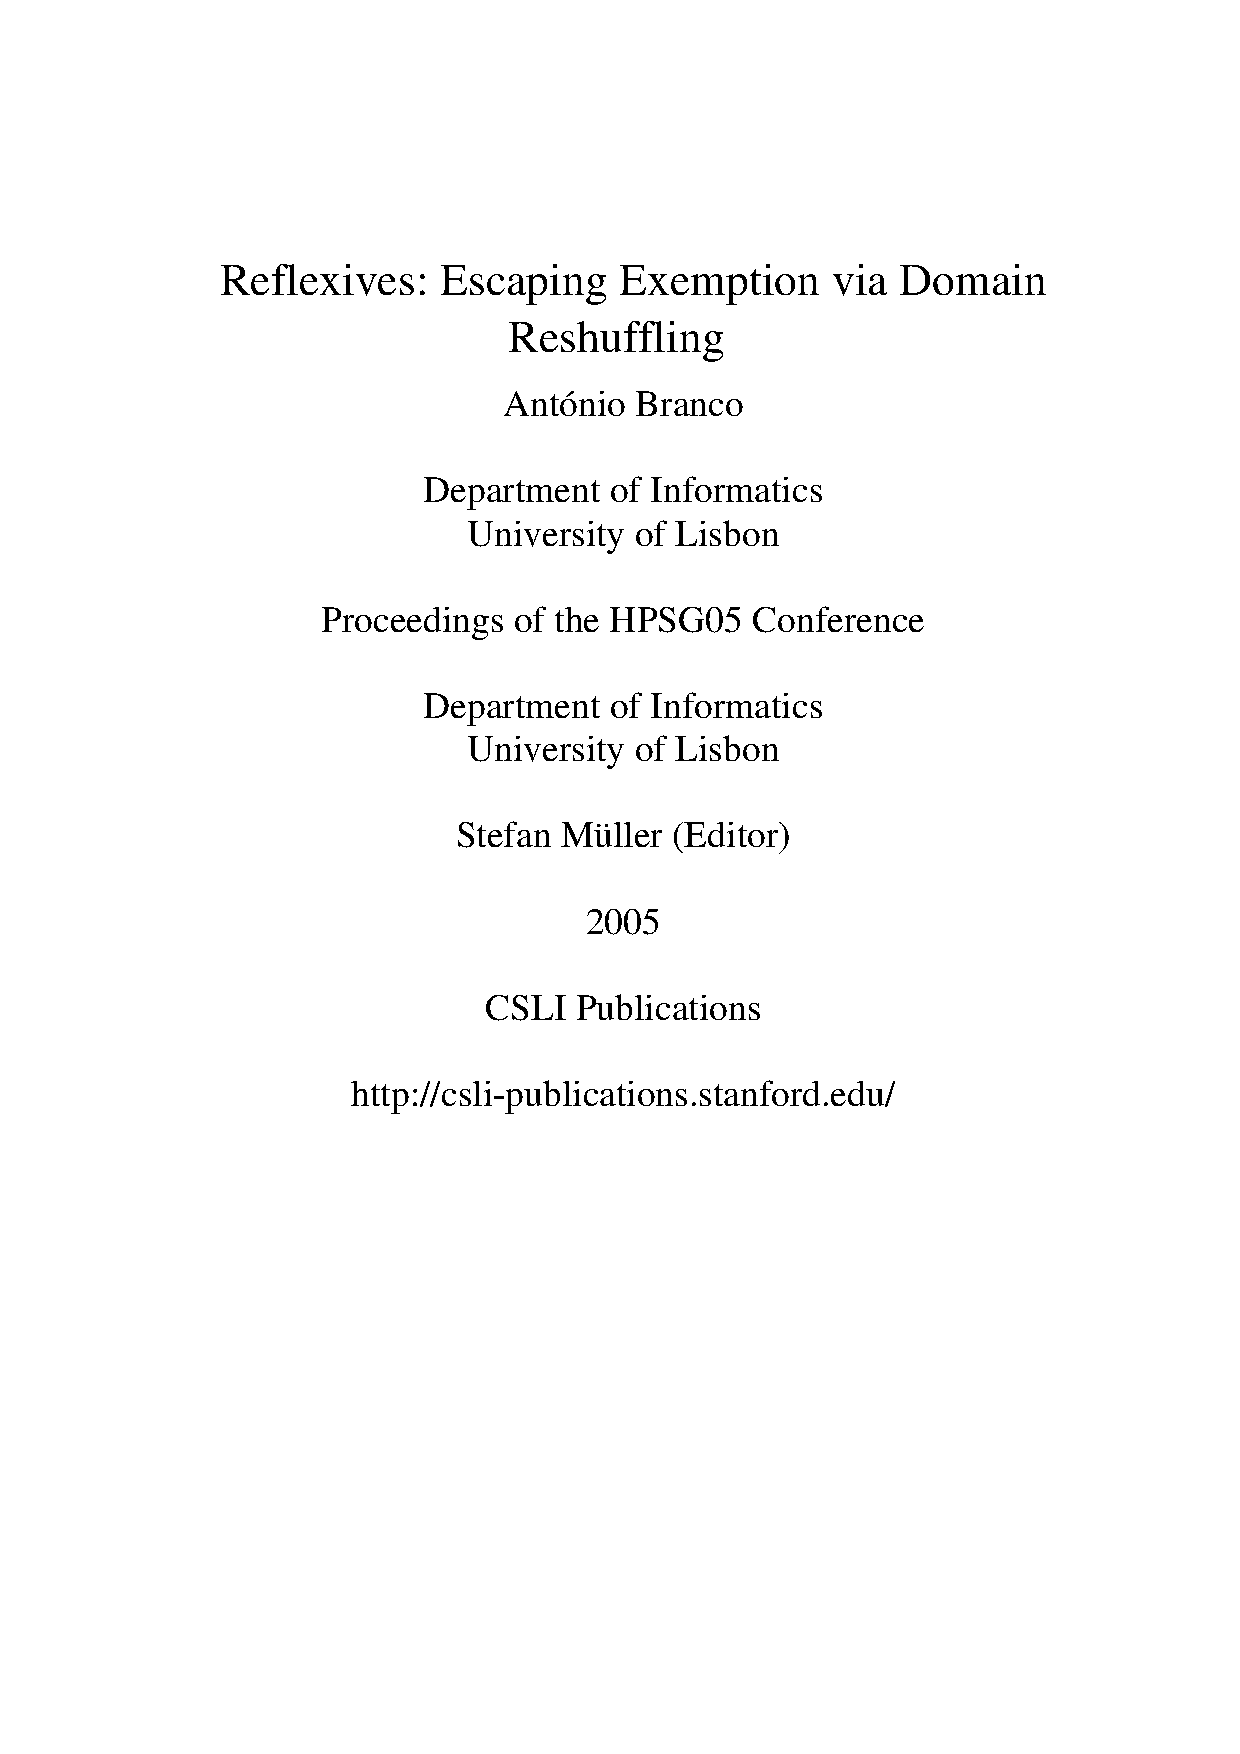
\includepdf[pages=-,pagecommand=\thispagestyle{plain},
            addtotoc={1,section,1,
            {Ant�nio Branco: Reflexives: Escaping Exemption via Domain Reshuffling},
             branco}]{branco.pdf}

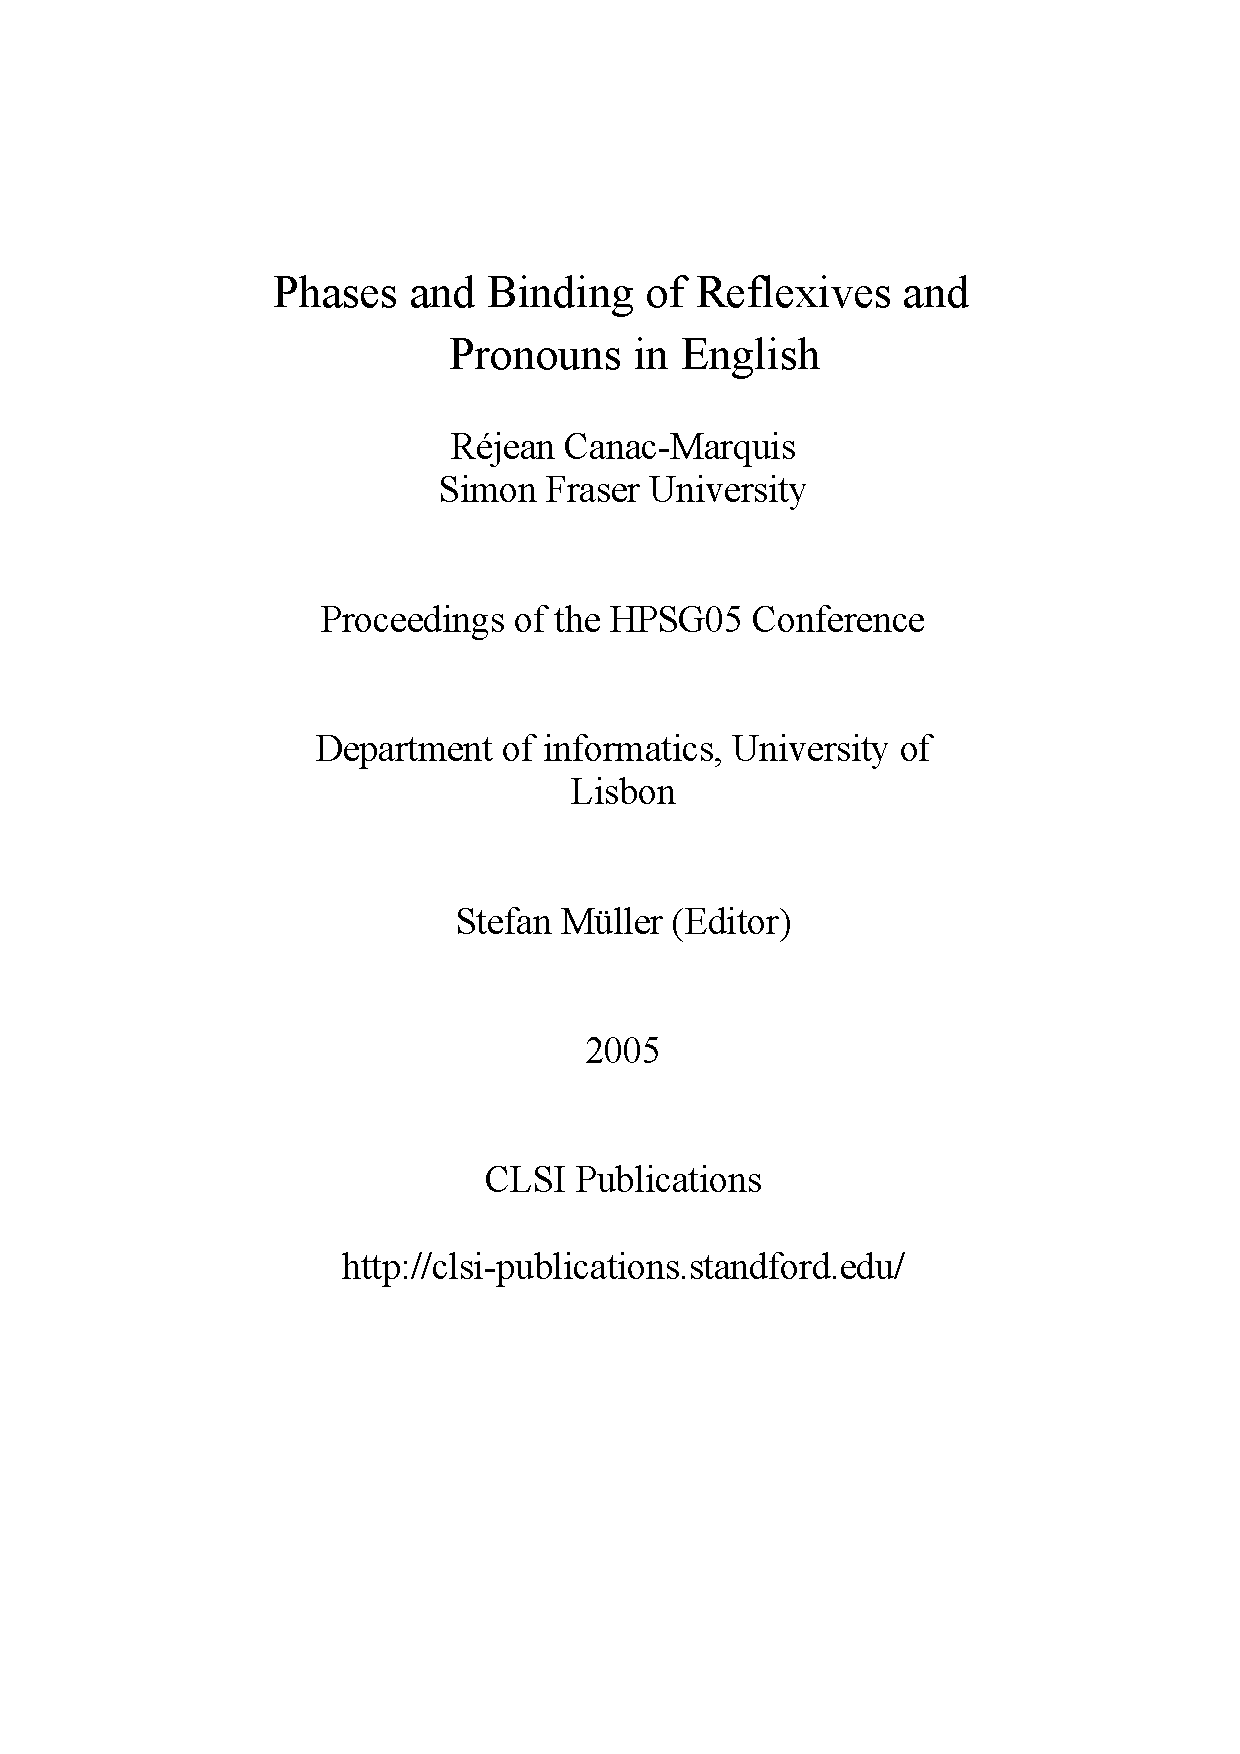
\includepdf[pages=-,pagecommand=\thispagestyle{plain},
            addtotoc={1,section,1,
            {R�jean Canac-Marquis: Phases and Binding of Reflexives and Pronouns in English},
             cm}]{canac-marquis.pdf}

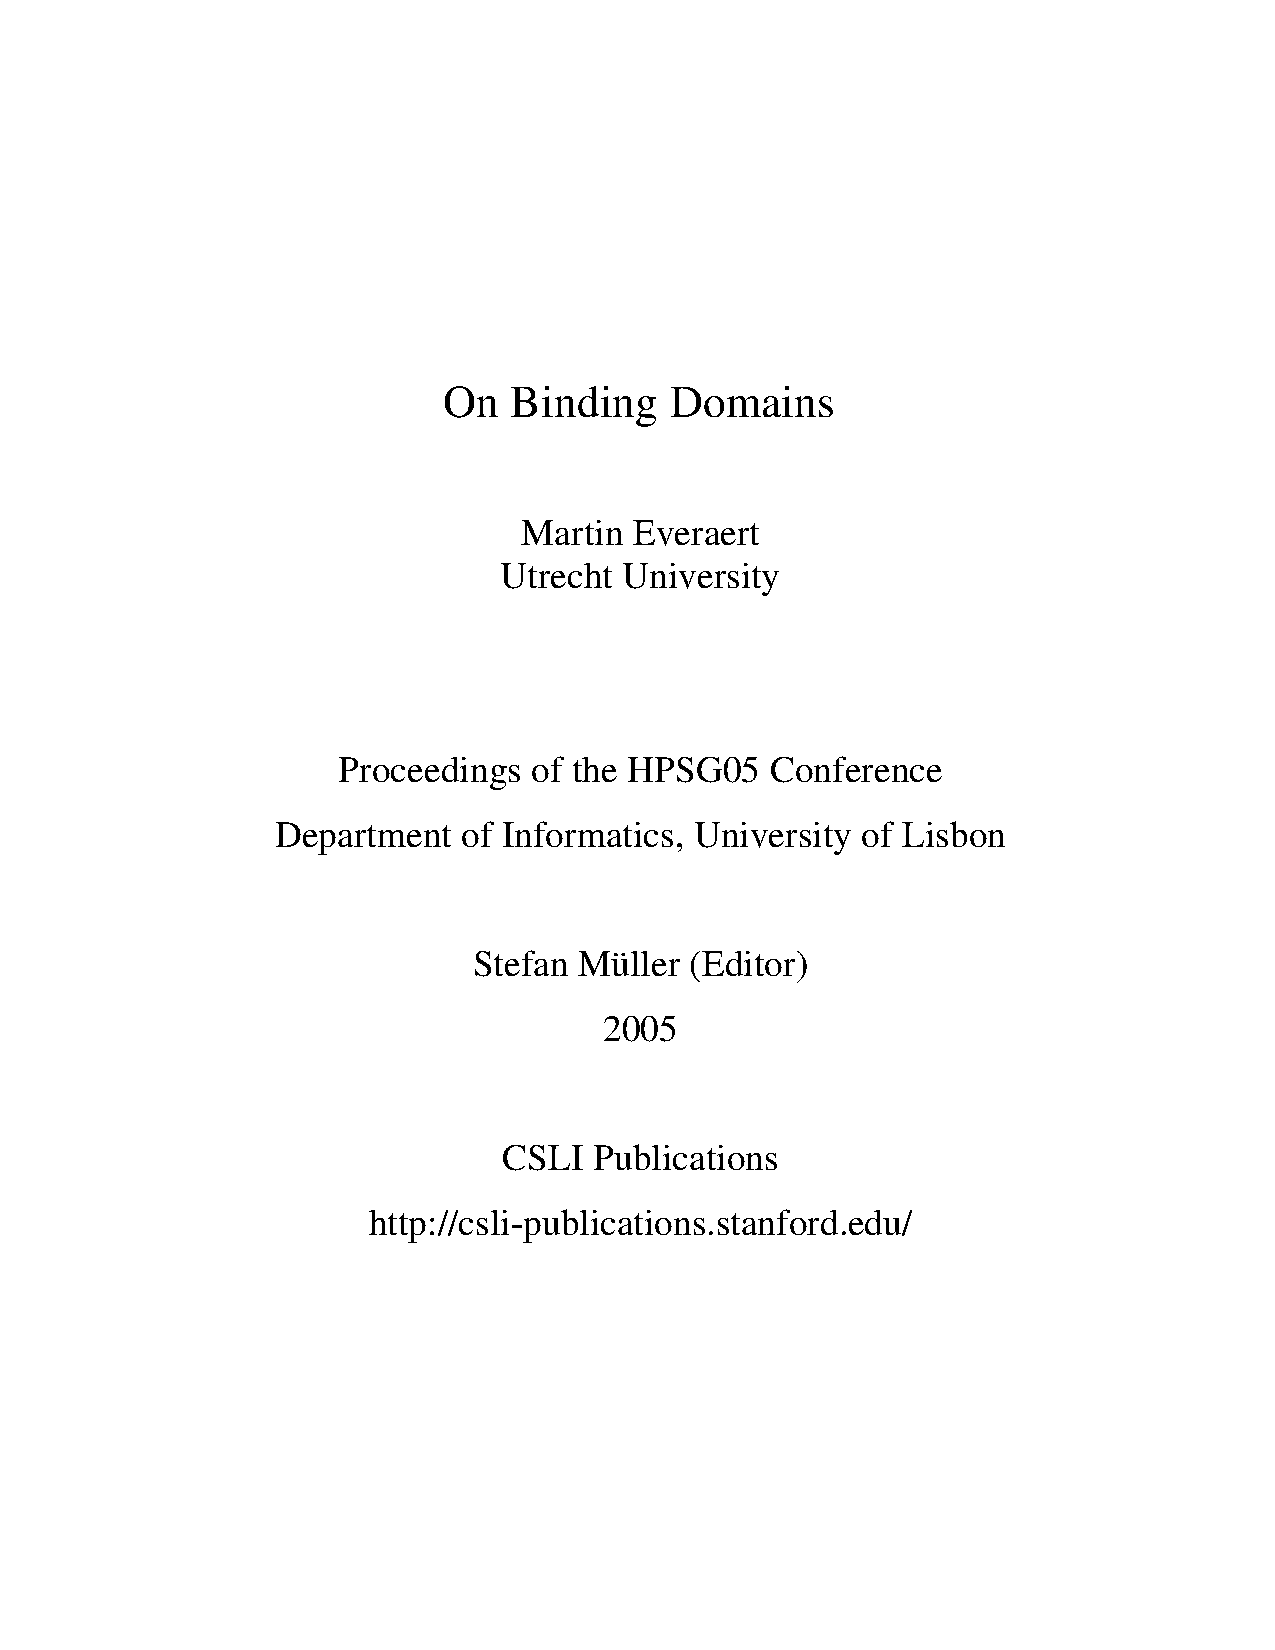
\includepdf[pages=-,pagecommand=\thispagestyle{plain},
            addtotoc={1,section,1,
            {Martin Everaert: On Binding Domains},
             everaert}]{everaert.pdf}



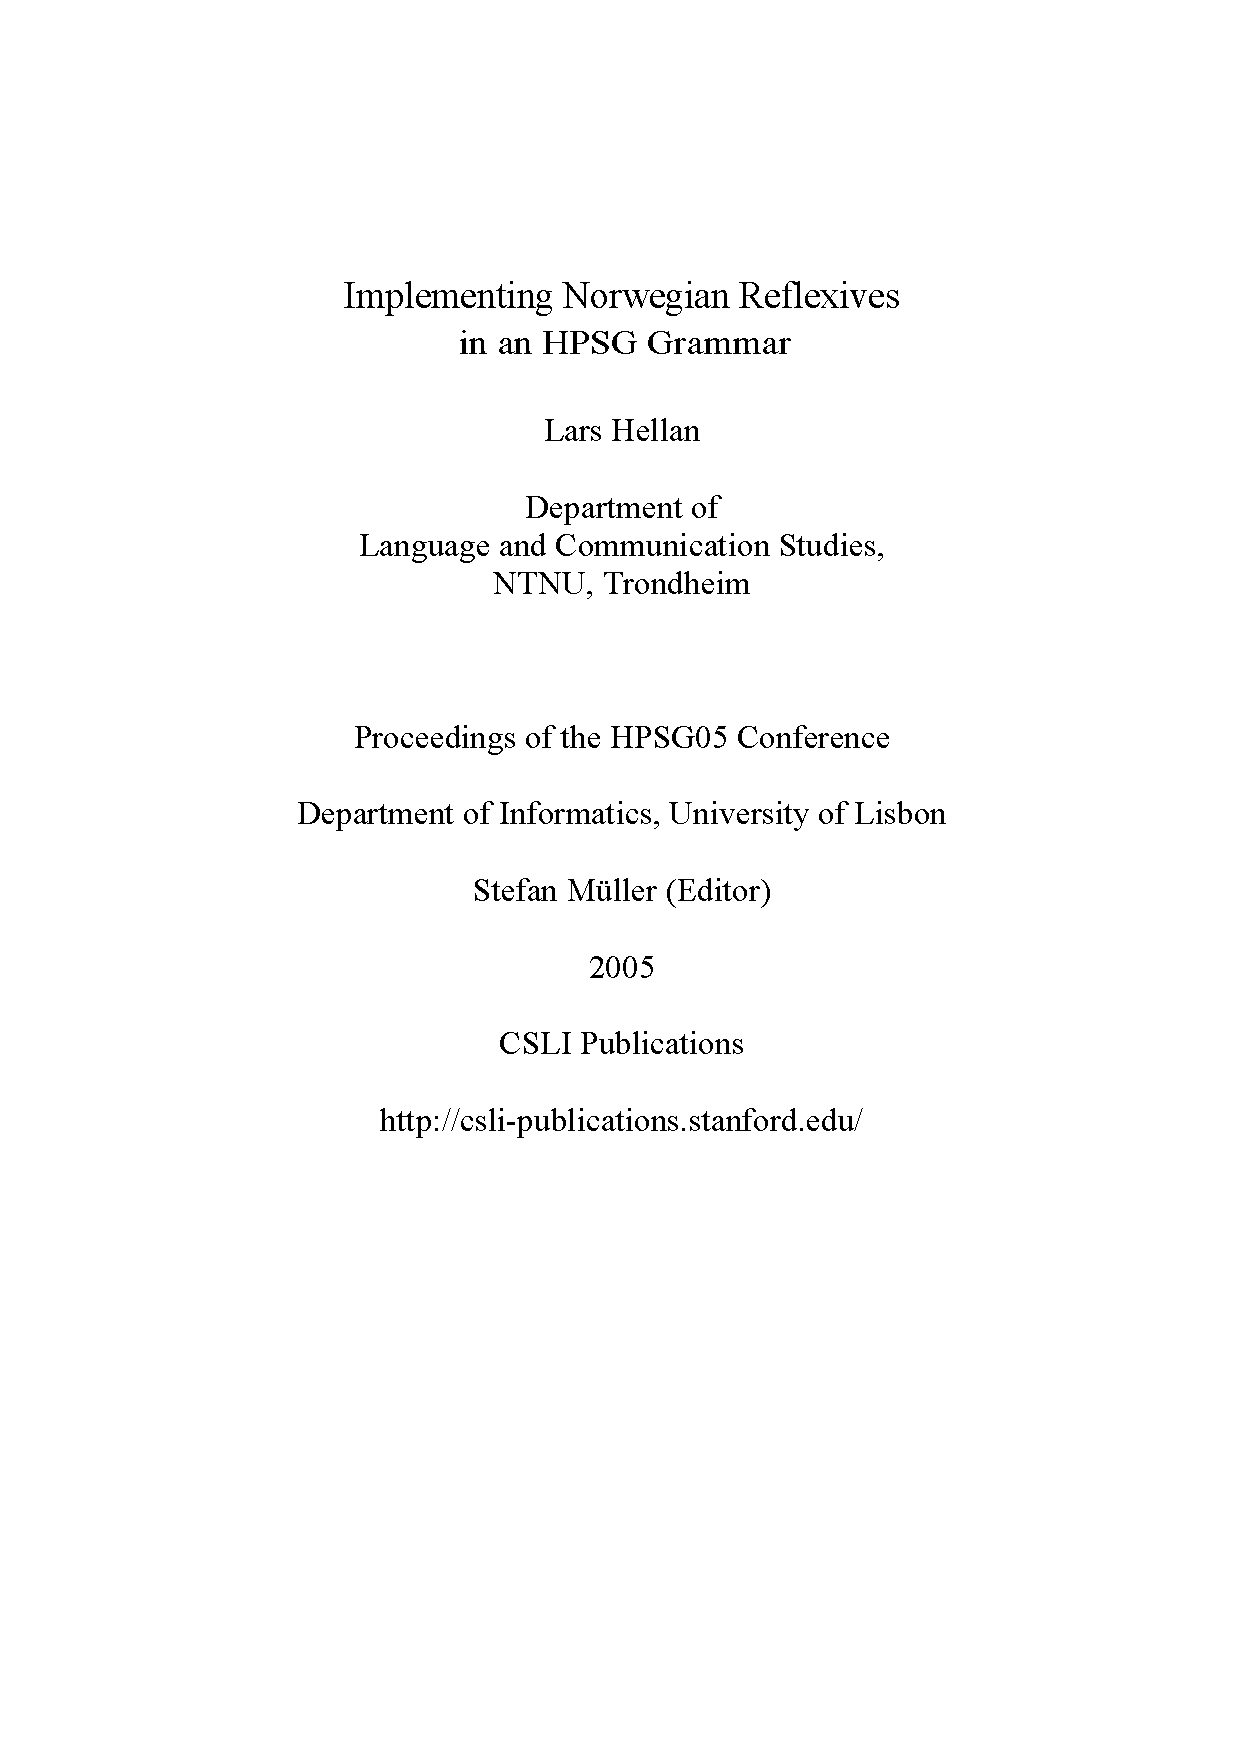
\includepdf[pages=-,pagecommand=\thispagestyle{plain},
            addtotoc={1,section,1,
            {Lars Hellan: Implementing Norwegian Reflexives in an HPSG Grammar},
             hellan}]{hellan.pdf}

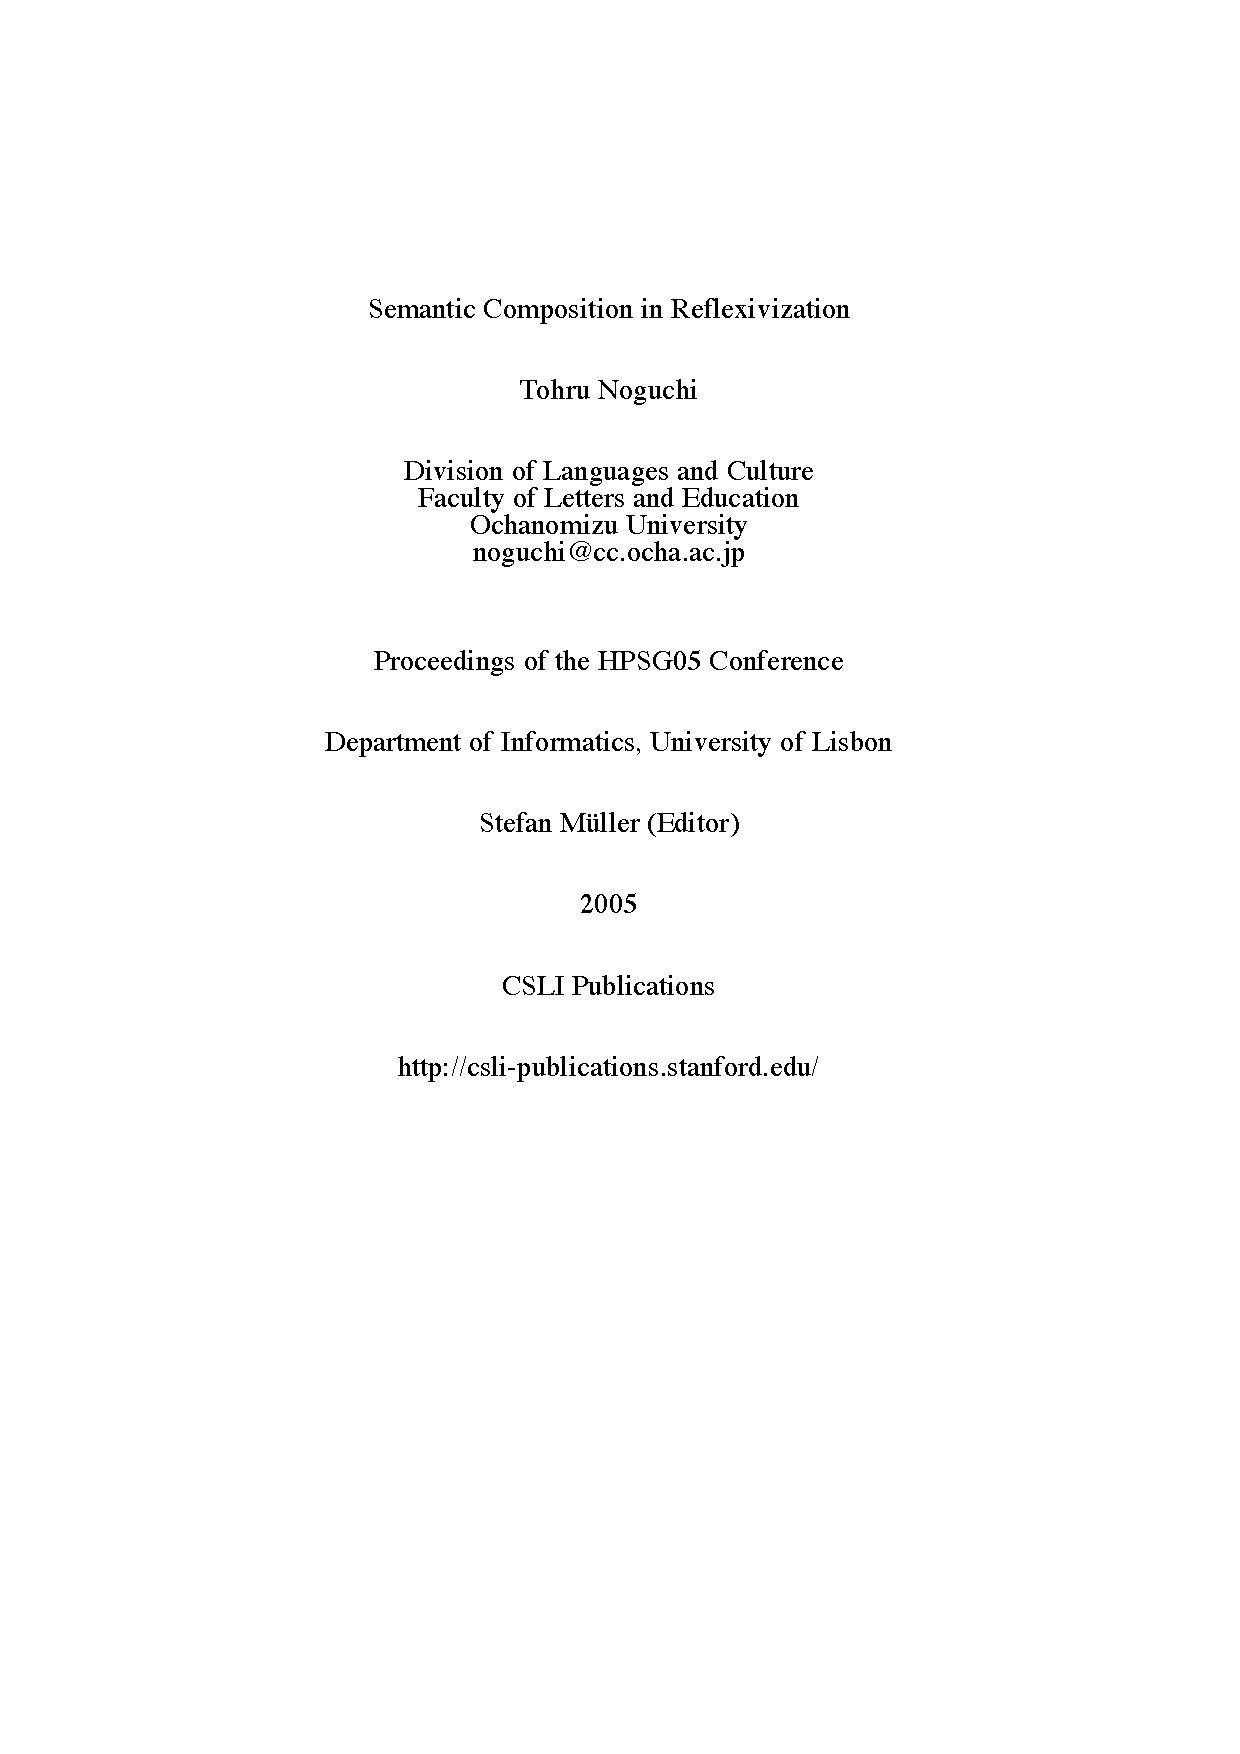
\includepdf[pages=-,pagecommand=\thispagestyle{plain},
            addtotoc={1,section,1,
            {Tohru Noguchi: Semantic Composition in Reflexivization},
             noguchi}]{noguchi.pdf}

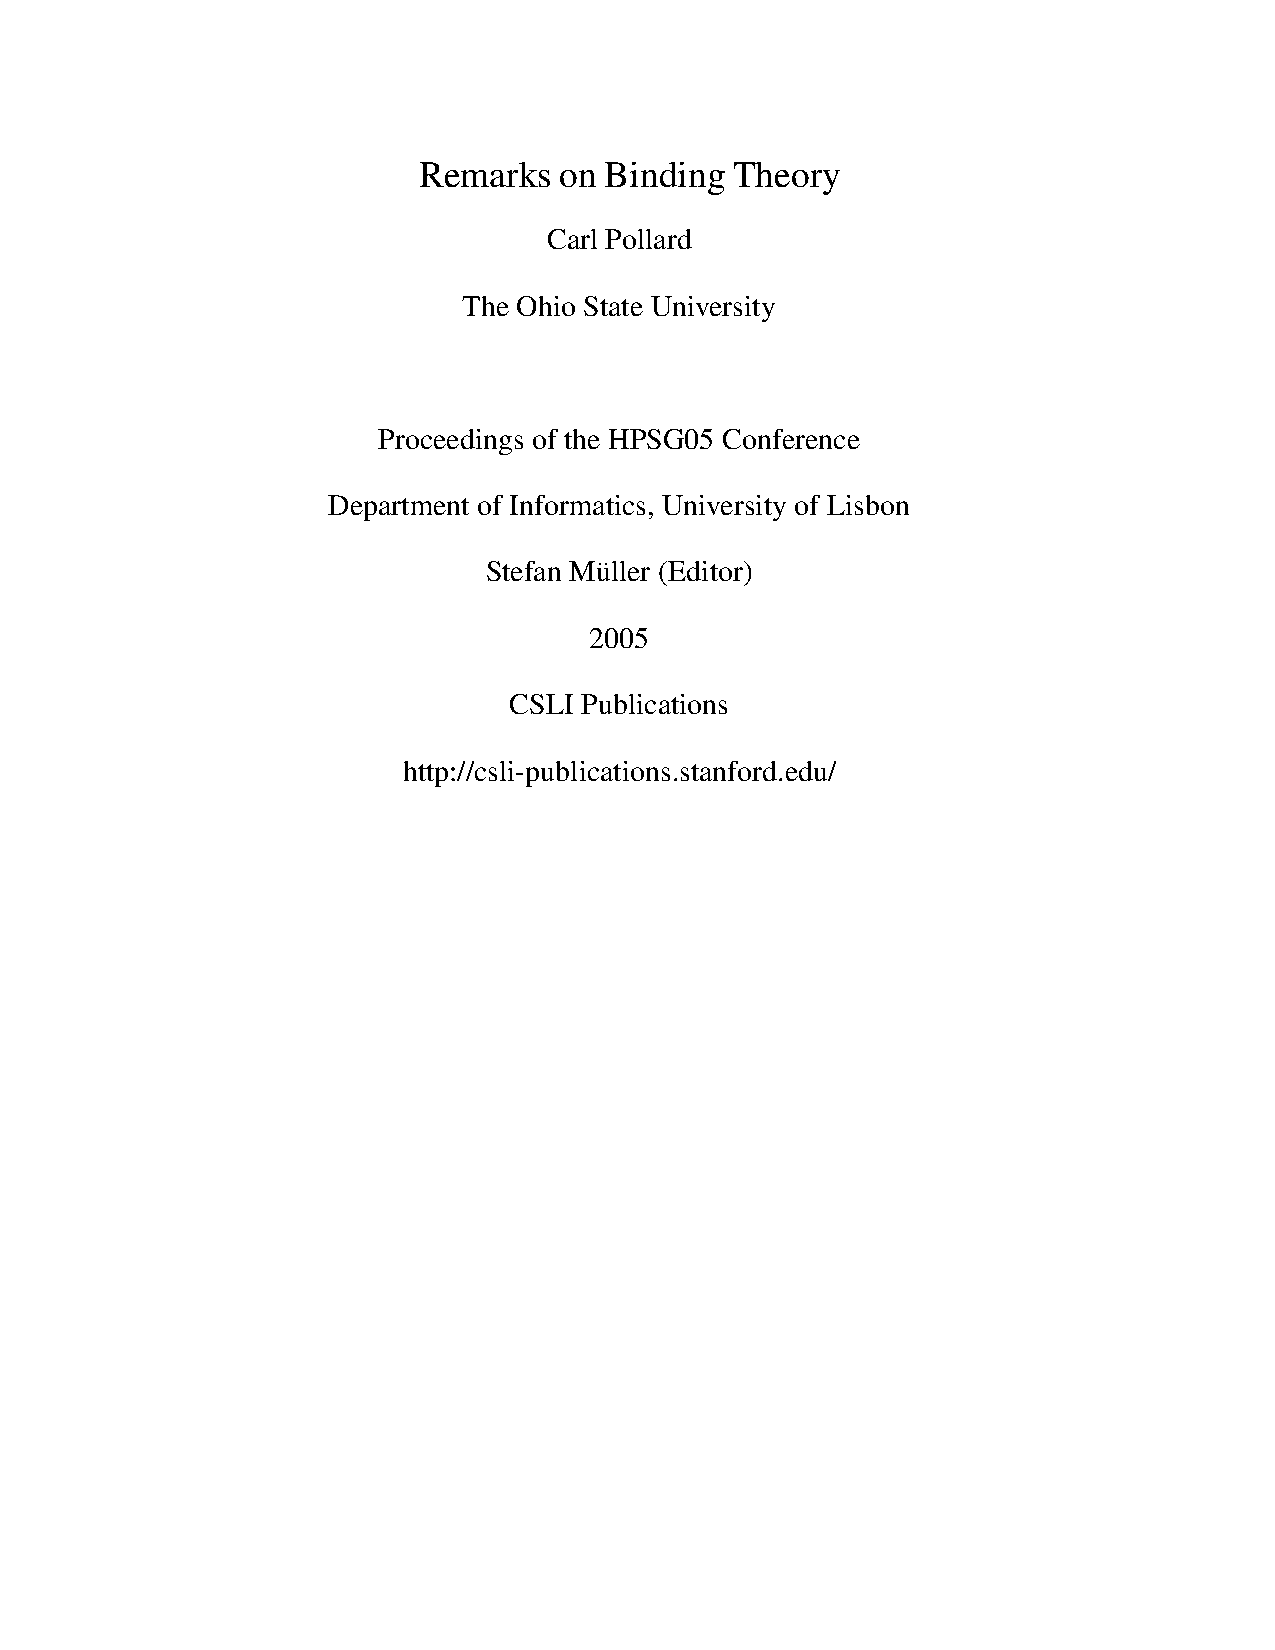
\includepdf[pages=-,pagecommand=\thispagestyle{plain},
            addtotoc={1,section,1,
            {Carl Pollard: Remarks on Binding Theory},
             pollard}]{pollard.pdf}


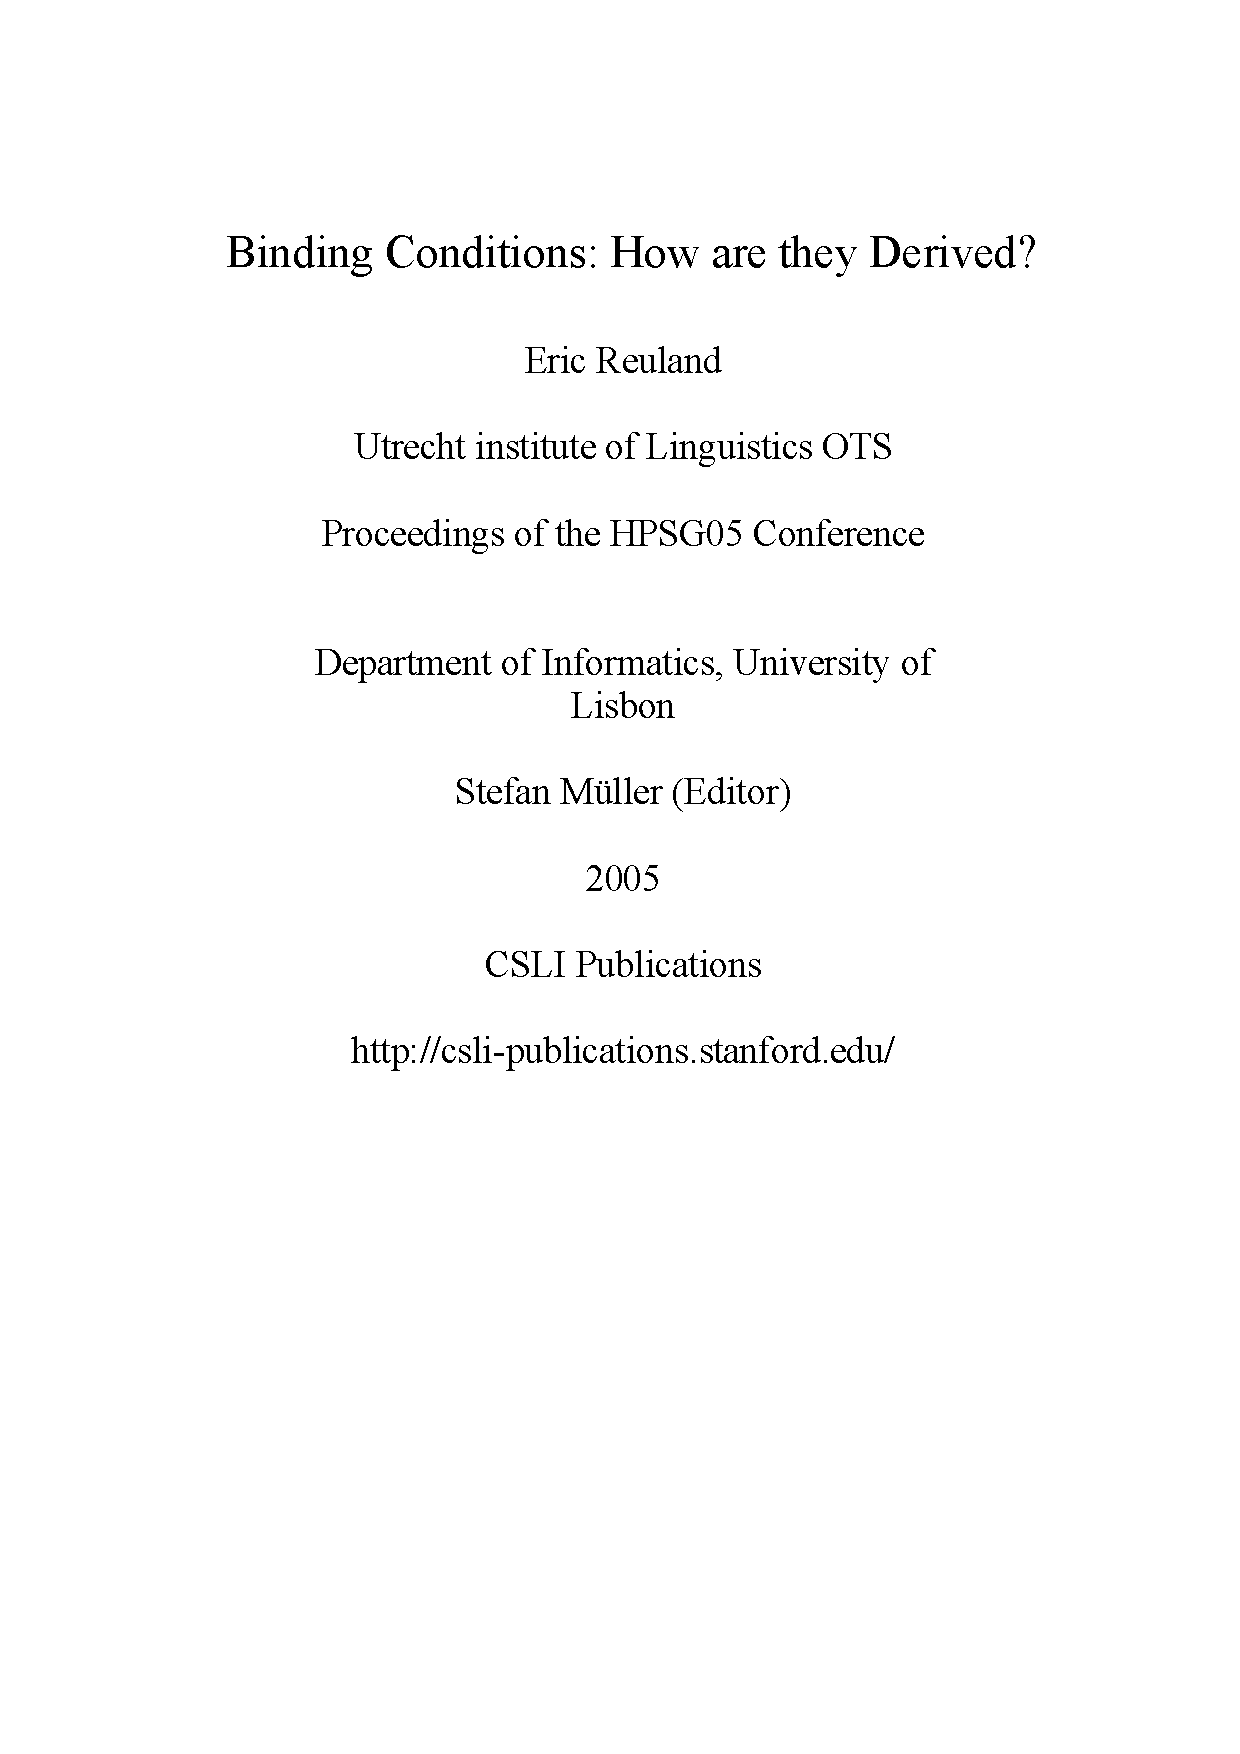
\includepdf[pages=-,pagecommand=\thispagestyle{plain},
            addtotoc={1,section,1,
            {Eric Reuland: Binding Conditions: How are they Derived?},
             reuland}]{reuland.pdf}


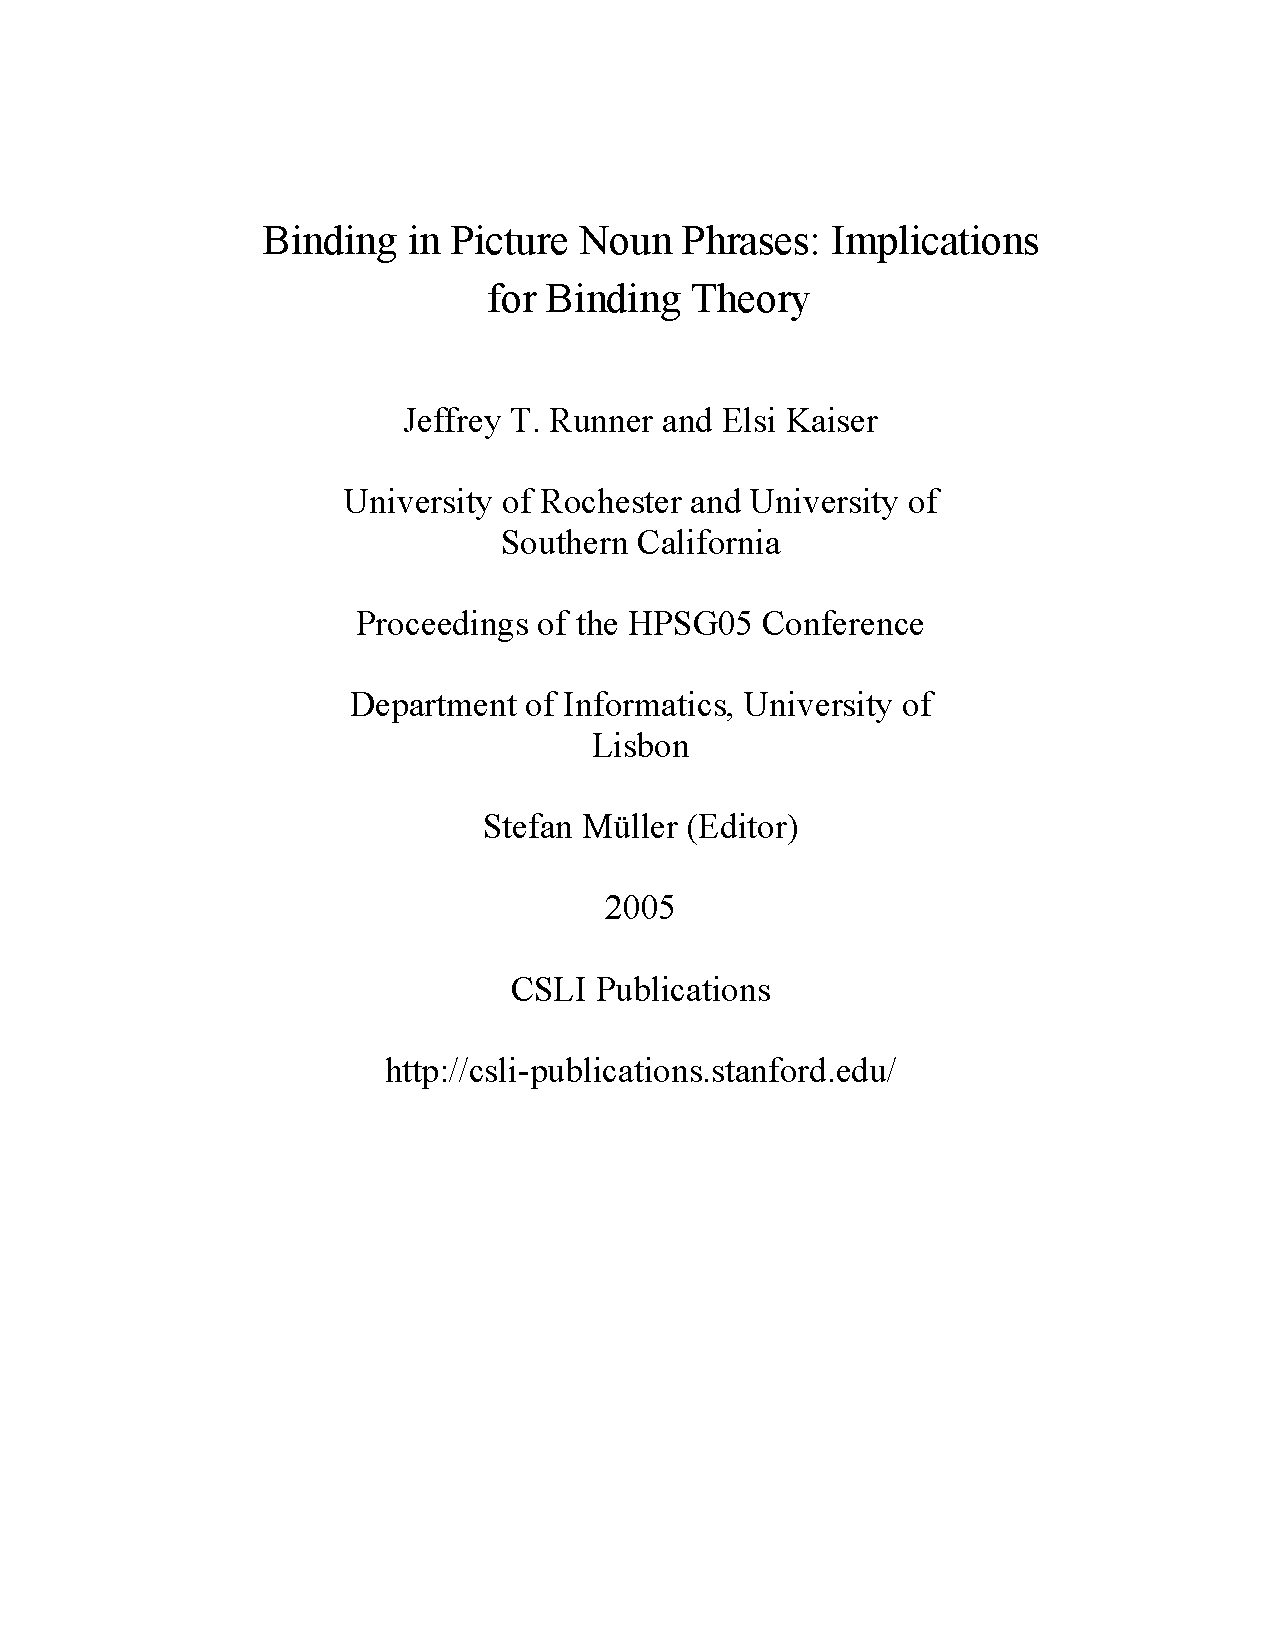
\includepdf[pages=-,pagecommand=\thispagestyle{plain},
            addtotoc={1,section,1,
            {Jeffrey T. Runner and Elsi Kaiser: Binding in Picture Noun Phrases: Implications for Binding Theory},
             rk}]{runner-kaiser.pdf}

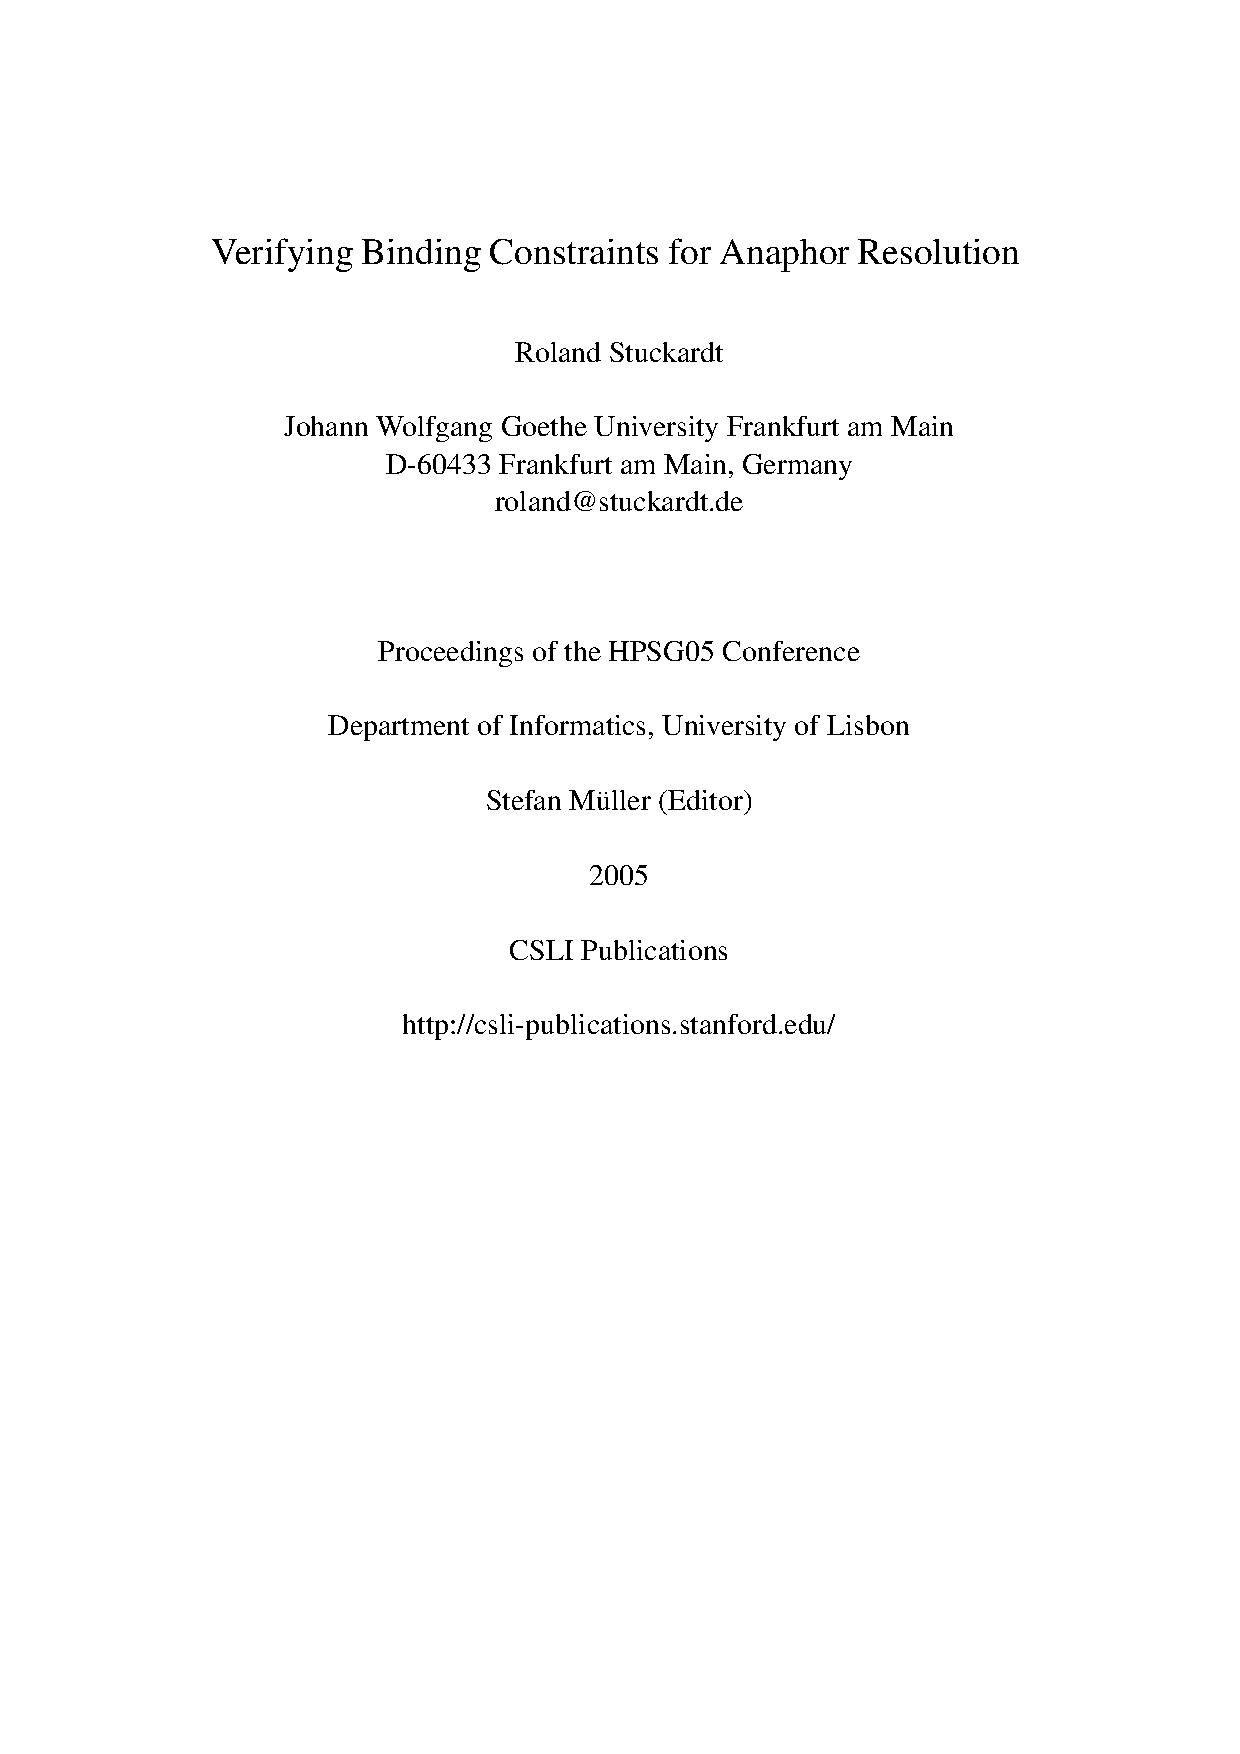
\includepdf[pages=-,pagecommand=\thispagestyle{plain},
            addtotoc={1,section,1,
            {Roland Stuckardt: Verifying Binding Constraints for Anaphor Resolution},
             stuckardt}]{stuckardt.pdf}



\end{document}

